\documentclass[a4paper,11pt,fontset=none,scheme=chinese]{ctexbook}
\ctexset{
  section/format = \Large\bfseries,
  today=old
}

% **************************************
% Language & Fonts
% **************************************
\input{lang}
\usepackage{CJKnumb}
%Mapping fixes endash & emdash
\newfontfamily\lmr{Latin Modern Roman}
\newfontfamily\courier{Courier New}

%\xeCJKsetcharclass{"0}{"2E7F}{0}
%\xeCJKsetcharclass{"2E80}{"FFFF}{1}
\DeclareTextAccent{\.}{EU1}{"0307}
%\DeclareTextAccent{\v}{EU1}{"030C}
%\DeclareTextAccent{\d}{EU1}{"0323}
%\DeclareTextAccent{\b}{EU1}{"0331}

\usepackage{etex}
\usepackage{metalogo,mflogo,texnames}
\usepackage{textcomp}

\usepackage[normalem]{ulem}
%\usepackage{xltxtra}                % load etex automatically

\hyphenation{Post-Script}

% **************************************
% Graphics
% **************************************
\usepackage{adjustbox}
\usepackage{graphicx, rotating}
\usepackage[svgnames, table]{xcolor}% put before pstricks, textpos, tikz

\DeclareGraphicsRule{.mps}{eps}{.mps}{}
% \graphicspath{{graph/}{img/}} mtex.cm works in project root, while the new mktex.cmd works in /src.
\graphicspath{{../graph/}{../img/}}

% **************************************
% Table
% **************************************
\usepackage{booktabs,longtable,multirow,tabularx,warpcol}

% **************************************
% Float
% **************************************
\usepackage{caption}
\DeclareCaptionType [fileext=loe]{example}[例][例目录]
%\usepackage{float}
%\newfloat{example}{tbph}{loe}
%\restylefloat*{example}
%\floatstyle{plain}
%\floatname{example}{例}
%\captionsetup[example]{position=top}
%\newcommand{\listofexamples}{\listof{example}{例目录}}
\usepackage{subfig}                 % put before fvrb-ex
\newsubfloat[position=bottom,listofformat=subsimple]{example}

% **************************************
% Structure
% **************************************
%\usepackage{xurl} % not working with url
%\PassOptionsToPackage{hyphens}{url}
\usepackage[
  bookmarksnumbered, 
  pdfencoding=auto, 
  pdfpagelayout=TwoPageRight,
  breaklinks, 
  colorlinks, 
  linkcolor=RoyalBlue, 
  urlcolor=blue]
{hyperref}
\usepackage{multicol}               % need etex
\usepackage{multind}
\makeindex{people}
\makeindex{org}
% replaced by ctexbook
% \usepackage{titlesec}

\newcommand{\lnotesauthor}{包 太 雷}
\newcommand{\lnotesversion}{v2.208}
\newcommand{\lnotesdate}{2025年9月}

% replaced by ctexbook
% \renewcommand{\contentsname}{目录}
\renewcommand{\listfigurename}{图目录}
\renewcommand{\listtablename}{表目录}
\renewcommand{\chaptername}{第\CJKnumber{\thechapter}章}
%\newcommand{\sectionname}{\thesection 节}
% \renewcommand{\figurename}{图}
% \renewcommand{\tablename}{表}
% \renewcommand{\appendixname}{附录{\thechapter}}
% \renewcommand{\bibname}{参考文献}
% \renewcommand{\indexname}{索引}

\renewcommand{\figureautorefname}{图}
\renewcommand{\tableautorefname}{表}
\renewcommand{\appendixautorefname}{附录}

% replaced by ctexbook
% \titleformat{\chapter}[block]{\center\Huge}{\chaptername}{20pt}{}
\makeatletter
\renewcommand{\tableofcontents}{%
\setlength{\columnsep}{2.5em}
%\setlength{\columnseprule}{.8pt}
\begin{multicols}{2}[\chapter*{\contentsname}]%
    \@starttoc{toc}%
\end{multicols}}
\makeatother

% **************************************
% Format
% **************************************
\usepackage{calc}
\usepackage{indentfirst,setspace}

%\usepackage{enumitem} % conflict with paralist
%\setlist[1]{labelindent=0.5\parindent,leftmargin=\parindent}
\usepackage{paralist}
\newenvironment{CompactEnum}{
\begin{enumerate}
    \setlength{\itemsep}{0pt}
    \setlength{\parsep}{0pt}
    \setlength{\parskip}{0pt}
}{\end{enumerate}}

\newenvironment{CompactItem}{
\begin{enumerate}
    \setlength{\itemsep}{0pt}
    \setlength{\parsep}{0pt}
    \setlength{\parskip}{0pt}
}{\end{enumerate}}

\newenvironment{CompactDesc}{
\begin{enumerate}
    \setlength{\itemsep}{0pt}
    \setlength{\parsep}{0pt}
    \setlength{\parskip}{0pt}
}{\end{enumerate}}

\usepackage{fancyvrb,listings,verbatim}

\VerbatimFootnotes
\usepackage{ldemo}

%\usepackage{framed}
\usepackage{marginnote}

%\renewcommand{\labelitemi}{\ensuremath{\bullet}}% xunicode changes the bullet

\makeatletter
\renewenvironment{quotation}{
    \list{}{
        \listparindent 2em
        \itemindent    \listparindent
        \rightmargin   \leftmargin
        \parsep        \z@ \@plus\p@
    }
    \item
}{
    \endlist
}
\makeatother

% **************************************
% Layout
% **************************************
\usepackage{fancyhdr}
\usepackage[absolute]{textpos}
\usepackage{varwidth}

\pagestyle{fancy}
\fancyhf{}
\fancyhead[LE,RO]{\thepage}
\fancyhead[RE]{\textit{\leftmark}}
\fancyhead[LO]{\textit{\rightmark}}
\fancypagestyle{plain}{             % set header and footer of plain pages
    \fancyhf{}
    \renewcommand{\headrulewidth}{0pt}
    \fancyfoot[LE,RO]{\thepage}
}

\makeatletter
\renewcommand{\cleardoublepage}{
    \clearpage
    \if@twoside \ifodd 
        \c@page
    \else
        \if@openrecto 
            \thispagestyle{empty}
            \vspace*{\fill}
            \begin{center}
                广告位招租
            \end{center}
            \vspace{\fill}
            \newpage
            \if@twocolumn
                \newpage
            \fi
        \fi 
    \fi\fi
}

\newif\if@openrecto
\makeatother

% **************************************
% Bibliography
% **************************************
\usepackage{chapterbib}
\usepackage[sectionbib,super,square,sort&compress]{natbib}

% **************************************
% Math
% **************************************
\usepackage{amsmath,amsfonts,amsthm,mathrsfs}

\begin{document}
\frontmatter
\include{front}                     % Front cover and title page
\include{copyright}

% Open right pages: title, dedication, TOC
\makeatletter
\@openrectotrue
\makeatother

\include{dedication}

% TOC, LOF, LOT
\tableofcontents

% Open any pages: LOF, LOT, forward, preface, acknowledgements, abbreviations
\makeatletter
\@openrectofalse
\makeatother

\listoffigures
\listoftables
\listofexamples

\renewcommand{\chaptermark}[1]{\markboth{#1}{}}
\onehalfspacing
\let\oldparskip\parskip
\addtolength{\parskip}{3pt}
\addtolength{\abovecaptionskip}{-3pt}
\addtolength{\belowcaptionskip}{-3pt}
\setlength{\parindent}{2em}

\include{forward}
\chapter{友人序}

This book was written by a friend Dr. Bao. The first version was published two years ago and this is the updated version. With many \LaTeX{} books around, is this book necessary? The answer is yes. This book is super cool. This is an advanced \LaTeX{} book and however it starts from basic and guides the readers to the most advanced tips. In addition, the style of the book is unique. It is half comments and half technical notes. If you missed the anecdotes, you miss many of the great materials.

Technical wise, the feature of the book is several fold: the presentation of digital printing technology and history, the description of software packages that can make paper/dissertation writing easier (such as how to convert a pdf to an eps file), the collection of tricks that otherwise take long time to master.

The book has 12 chapters with two Appendices. With Chapter 1 as introduction of history and Chapter 2 as introduction of \LaTeX{} as a whole from a "hello world" example, Chapter 3 s on fonts. This is a surprise arrangement and it showcases the author as an aesthete more than a software engineer. PS, \LaTeX{} lovers are more or less aesthetes, aren't they? Mathematic expressions are described in Chapter 4 and Chapter 5 is on figures. The next three chapters are not usually seen in \LaTeX{} books and they are: Metapost, PSTricks and PGF. Honestly speaking, I have not read these three chapters. Tables are mentioned in Chapter 9 and it is super useful. After reading Chapter 9, one knows how to rotate a table, how to make a long table, a wide table, etc. Chapter 10 is on structure. Chapter 11 is on printing. It gives a graphic explanation on page margins. Finally chapter 12 is on other applications such as Beamer for slides show, CV template, and letter template. The Appendices are of much use as well: Appendix A is about packages. Appendix B is on brief history of printing.

Nontechnical wise, the book is super funny with its anecdotes. The writing is in Chinese and many historical poems were re-shaped in preface. In Chapter 1, when history of digital printing was described, names and stories of computer scientists who devoted their energy in making \LaTeX{}, Adobe and etc were told. The author was obsessed with each person's background, school and degree. In footnotes, you will see sth like this 1: Ph.D. from Cambridge or PhD from MIT, etc.

The only disadvantage of this book is it is in Chinese and thus, the language limits its readers. On the other hand, with English as second language, can a book in English be that funny?

\begin{flushright}
Dr. Fan Lingling \\
Augest 26, 2013
\end{flushright}

\include{preface}
\include{preface-old}
\chapter{致谢}

在本文的写作过程中,我得到了众多网友的帮助和指点,各位反动学术权威的关心和鼓励。没有你们的帮助,包老师形只影单单枪匹马马不停蹄也难以完成这件超出本人能力的事情。

在此包老师依据我国法律\footnote{《中华人民共和国感谢法》,2010年3月12日。},首先郑重感谢党和政府的栽培,国家和人民的养育,以及有关部门的领导。感谢铁岭 TV,辽宁 TV,将来还有可能感谢 CCTV。

其次将网友们的名单公诸于众,以彰显社会良知、公民勇气。以下排名不分先后,其中多数网友来自水木清华 BBS \TeX 版和 C\TeX 论坛。

\begin{multicols}{3}
\noindent
boltomli\\
careworn\\
Dieken\\
donated\\
Felix Lee\\
gaozhch\\
garfileo\\
GasinAn\\
hkkhhk\\
Hongdong Ji\\
IMB\\
jjgod\\
Kov Chai\\
Langpku\\
LittleLeo\\
maming\\
meteorrain\\
milksea\\
Naitree Zhu\\
northwater\\
PaladinHL\\
PiscesGold\\
primenumber\\
sesame\\
shenshou246\\
shuangwen\\
snoopyzhao\\
Sofoot\\
tex\\
Wang Chenlin\\
Xiao Zigang\\
Xubuntu\\
yakun\\
Yiming\\
yli\\
yyzz11\\
zoho\\
贾朋\\
张晓南\\
赵梓琪
\end{multicols}

特别感谢范、沈、王、李、林诸位教授的鼓励、意见与建议。

也借机感谢一下4.80\footnote{166.111.4.80 是清华大学校园网早期一个重要的 FTP 站点。}前站长 Jonny 和水木清华 BBS 前站长 Leeward。十余年前,在我开始浸淫于电脑网络时,这两位高手对我有很大的启发和影响。虽然两位高人淡出公众视野已久,但是他们为人民服务的精神却依然值得我们缅怀与尊敬。

最后还要感谢家人的理解和支持。老妻把她的博士论文给我当作学习 \LaTeX 的试验品;大女儿把她的玉照给我当作插图样板;小女儿把她的名字给我放在献辞页。


\makeatletter
\@openrectotrue
\makeatother
\mainmatter
\renewcommand{\chaptermark}[1]{\markboth{\chaptername: #1}{}}
\renewcommand{\sectionmark}[1]{\markright{\thesection: #1}}

%People
%\newcommand{\indexAho}{\index{people}{Aho@Alfred V. Aho, 阿尔佛雷德·艾侯}}
%\newcommand{\indexFourer}{\index{people}{Fourer@Robert Fourer, 罗伯特·福瑞尔}}
%\newcommand{\indexGay}{\index{people}{Gay@David M. Gay, 大卫·给}}
%\newcommand{\indexRitchie}{\index{people}{Ritchie@Dennis M. Ritchie, 丹尼斯·瑞奇}}
%\newcommand{\indexWeinberger}{\index{people}{Weinberger@Peter J. Weinberger, 彼得·温伯格}}
\newcommand{\indexBarclay}{\index{people}{Barclay@Robert Barclay, 罗伯特·巴克雷}}
\newcommand{\indexBernersLee}{\index{people}{Berners-Lee@Tim J. Berners-Lee, 蒂姆·伯纳斯-李}}
\newcommand{\indexBerry}{\index{people}{Berry@Karl Berry, 卡尔·白瑞}}
\newcommand{\indexCarlisle}{\index{people}{Carlisle@David P. Carlisle, 大卫·卡利斯}}
\newcommand{\indexCarlson}{\index{people}{Carlson@Chester F. Carlson, 切斯特·卡尔森}}
\newcommand{\indexCassatt}{\index{people}{Cassatt@Mary S. Cassatt, 玛丽·卡萨特}}
\newcommand{\indexCochran}{\index{people}{Cochran@Steven D. Cochran, 斯蒂文·寇克阮}}
\newcommand{\indexDaly}{\index{people}{Daly@Patrick W. Daly, 派垂克·达利}}
\newcommand{\indexDanaux}{\index{people}{Danaux@Xavier Danaux, 夏卫·丹诺克}}
\newcommand{\indexDupuis}{\index{people}{Dupuis@Étienne Dupuis, 艾提纳·杜普斯}}
\newcommand{\indexDurer}{\index{people}{Durer@Albrecht Dürer, 阿尔布雷希特·丢勒}}
\newcommand{\indexEvans}{\index{people}{Evans@David C. Evans, 大卫·埃文斯}}
\newcommand{\indexFairbairns}{\index{people}{Fairbairns@Robin Fairbairns, 罗宾·费尔贝恩}}
\newcommand{\indexFear}{\index{people}{Fear@Simon Fear, 西门怕怕}}
\newcommand{\indexFuchs}{\index{people}{Fuchs@David R. Fuchs, 大卫·福克斯}}
\newcommand{\indexGainsborough}{\index{people}{Gainsborough@Thomas Gainsborough, 托马斯·艮斯博罗}}
\newcommand{\indexGeschke}{\index{people}{Geschke@Charles M. Geschke, 查尔斯·哥谢克}}
\newcommand{\indexGirou}{\index{people}{Girou@Denis Girou, 丹尼斯·杰若}}
\newcommand{\indexGoldfarb}{\index{people}{Goldfarb@Charles F. Goldfarb, 查尔斯·歌德法布}}
\newcommand{\indexGoossens}{\index{people}{Goossens@Michel Goossen, 迈克尔·古神}}
\newcommand{\indexGoya}{\index{people}{Goya@Francisco Goya, 弗朗西斯科·戈雅}}
\newcommand{\indexGratzer}{\index{people}{Gratzer@George Grätzer, 乔治·格拉兹}}
\newcommand{\indexGutenberg}{\index{people}{Gutenberg@Johannes Gutenberg, 约翰内斯·古腾堡}}
\newcommand{\indexHagen}{\index{people}{Hagen@Hans Hagen, 汉斯·哈根}}
\newcommand{\indexHellmich}{\index{people}{Hellmich@Waldemar Hellmich, 瓦尔德玛·海米}}
\newcommand{\indexHigonnet}{\index{people}{Higonnet@René A. Higonnet, 勒内·希格涅特}}
\newcommand{\indexHobby}{\index{people}{Hobby@John D. Hobby, 约翰·爱好}}
\newcommand{\indexHoekwater}{\index{people}{Hoekwater@Taco Hoekwater, 塔克·毫克水}}
\newcommand{\indexHoover}{\index{people}{Hoover@Herbert Hoover, 赫伯特·胡佛}}
\newcommand{\indexHopfer}{\index{people}{Hopfer@Daniel Hopfer, 丹尼尔·霍卜弗}}
\newcommand{\indexJobs}{\index{people}{Jobs@Steve Jobs, 斯蒂夫·乔布斯}}
\newcommand{\indexJoy}{\index{people}{Joy@Bill N. Joy, 比尔·乔伊}}
\newcommand{\indexKastenbein}{\index{people}{Kastenbein@Karl Kastenbein, 卡尔·卡斯腾本}}
\newcommand{\indexKern}{\index{people}{Kern@Uwe Kern, 尤伟·科恩}}
\newcommand{\indexKernighan}{\index{people}{Kernighan@Brian W. Kernighan, 布莱恩·科尼汉}}
\newcommand{\indexKew}{\index{people}{Kew@Jonathan Kew, 乔纳森·酷}}
\newcommand{\indexKlic}{\index{people}{Klic@Karl Klíč, 卡尔·克里克}}
\newcommand{\indexKniagininski}{\index{people}{Kniagininski@Peter Kniagininski, 彼得·可怜人斯基}}
\newcommand{\indexKnuth}{\index{people}{Knuth@Donald E. Knuth, 高德纳}}
\newcommand{\indexLamport}{\index{people}{Lamport@Leslie Lamport, 莱斯利·兰泡特}}
\newcommand{\indexLanston}{\index{people}{Lanston@Tolbert Lanston, 托伯特·兰斯顿}}
\newcommand{\indexLemberg}{\index{people}{Lemberg@Werner Lemberg, 维尔纳·林伯格}}
\newcommand{\indexLesenko}{\index{people}{Lesenko@Sergey Lesenko, 瑟基·莱森科}}
\newcommand{\indexLevy}{\index{people}{Levy@Silvio Levy, 斯维·勒维}}
\newcommand{\indexLichtenberg}{\index{people}{Lichtenberg@Georg C. Lichtenberg, 乔治·里腾堡}}
\newcommand{\indexLorie}{\index{people}{Lorie@Raymond Lorie, 雷蒙德·劳里}}
\newcommand{\indexMarkey}{\index{people}{Markey@Nicolas Markey, 尼古拉斯·马克}}
\newcommand{\indexMcIlroy}{\index{people}{McIlroy@Malcolm D. McIlroy, 马尔考姆·麦克罗伊}}
\newcommand{\indexMerayHorvath}{\index{people}{Meray-Horvath@C. Méray Horváth, 莫雷-霍瓦斯}}
\newcommand{\indexMergenthaler}{\index{people}{Mergenthaler@Ottmar Mergenthaler, 奥特玛·摩根泰勒}}
\newcommand{\indexMiletic}{\index{people}{Miletic@Vedran Miletić, 维特恩·米尔提克}}
\newcommand{\indexMittelbach}{\index{people}{Mittelbach@Frank Mittelbach, 弗兰克·米特巴赫}}
\newcommand{\indexMorris}{\index{people}{Morris@Robert H. Morris, 罗伯特·莫里斯}}
\newcommand{\indexMoses}{\index{people}{Moses@Brooks Moses, 布鲁克斯·摩西}}
\newcommand{\indexMosher}{\index{people}{Mosher@Edward Mosher, 爱德华·莫谢}}
\newcommand{\indexMoyroud}{\index{people}{Moyroud@Louis M. Moyroud, 路易·毛绒的}}
\newcommand{\indexNewell}{\index{people}{Newell@Martin Newell, 马丁·牛维尔}}
\newcommand{\indexOberdiek}{\index{people}{Oberdiek@Heiko Oberdiek, 黑口·奥本迪克}}
\newcommand{\indexOetiker}{\index{people}{Oetiker@Tobias Oetiker, 托比·欧提克}}
\newcommand{\indexOostrum}{\index{people}{van Oostrum@Piet van Oostrum, 皮特·范·奥斯图姆}}
\newcommand{\indexOssanna}{\index{people}{Ossanna@Joseph F. Ossanna, 约瑟夫·奥萨纳}}
\newcommand{\indexOstwald}{\index{people}{Ostwald@Wilhelm Ostwald, 威廉·奥斯特瓦尔德}}
\newcommand{\indexPakin}{\index{people}{Pakin@Scott Pakin, 斯考特·培钦}}
\newcommand{\indexPatashnik}{\index{people}{Patashnik@Oren Patashnik, 奥润·帕塔尼克}}
\newcommand{\indexPorstmann}{\index{people}{Porstmann@Walter Porstmann,瓦尔特·泡茨曼}}
\newcommand{\indexRahtz}{\index{people}{Rahtz@Sebastian P. Rahtz, 塞巴斯蒂安·拉兹}}
\newcommand{\indexReagon}{\index{people}{Reagon@Ronald Reagan, 罗纳德·里根}}
\newcommand{\indexReckdahl}{\index{people}{Reckdahl@Keith Reckdahl, 凯斯·瑞克道}}
\newcommand{\indexReid}{\index{people}{Reid@Brian K. Reid, 布莱恩·瑞得}}
\newcommand{\indexRobertson}{\index{people}{Robertson@Will Robertson, 威尔·罗伯特森}}
\newcommand{\indexRochester}{\index{people}{Rochester@Wayne A. Rochester, 韦恩·罗彻斯特}}
\newcommand{\indexRokicki}{\index{people}{Rokicki@Tomas Rokicki, 托马斯·若奇奇}}
\newcommand{\indexRubel}{\index{people}{Rubel@Ira W. Rubel, 伊雷·鲁卜}}
\newcommand{\indexSaltzer}{\index{people}{Saltzer@Jerome H. Saltzer, 杰若米·萨尔兹}}
\newcommand{\indexSchandl}{\index{people}{Schandl@Bernd Schandl, 波得·辛得}}
\newcommand{\indexSchopf}{\index{people}{Schopf@Rainer Schöpf, 雨人·肖普弗}}
\newcommand{\indexSenefelder}{\index{people}{Senefelder@Alois Senefelder, 阿劳斯·塞尼菲尔德}}
\newcommand{\indexShamos}{\index{people}{Shamos@Michael I. Shamos, 迈克尔·沙毛斯}}
\newcommand{\indexSommerfeldt}{\index{people}{Sommerfeldt@Axel Sommerfeldt, 艾克赛·萨摩非特}}
\newcommand{\indexSpivak}{\index{people}{Spivak@Michael D. Spivak, 迈克尔·斯匹维克}}
\newcommand{\indexSproull}{\index{people}{Sproull@Robert F. Sproull, 罗伯特·斯普罗}}
\newcommand{\indexStallman}{\index{people}{Stallman@Richard M. Stallman, 理查德·斯托曼}}
\newcommand{\indexStarkweather}{\index{people}{Starkweather@Gary K. Starkweather, 盖瑞·斯塔克维}}
\newcommand{\indexSutherland}{\index{people}{Sutherland@Ivan E. Sutherland, 伊凡·苏泽兰}}
\newcommand{\indexTantau}{\index{people}{Tantau@Till Tantau, 提·谭陶}}
\newcommand{\indexTaylor}{\index{people}{Taylor@Philip Taylor, 菲利普·泰勒}}
\newcommand{\indexThompson}{\index{people}{Thompson@Paul A. Thompson, 保罗·汤普森}}
\newcommand{\indexUry}{\index{people}{Ury@Lesser Ury, 莱瑟·尤里}}
\newcommand{\indexVanZandt}{\index{people}{van Zandt@Timothy van Zandt, 提摩西·范·赞特}}
\newcommand{\indexVeytsman}{\index{people}{Veytsman@Boris Veytsman, 波瑞斯·韦茨曼}}
\newcommand{\indexVonSiegen}{\index{people}{von Siegen@Ludwig von Siegen, 路德维希·冯·希根}}
\newcommand{\indexVoss}{\index{people}{Voss@Herbert Voß, 赫伯特·沃斯}}
\newcommand{\indexWarnock}{\index{people}{Warnock@John E. Warnock, 约翰·沃诺克}}
\newcommand{\indexWicks}{\index{people}{Wicks@Mark A. Wicks, 马克·维克斯}}
\newcommand{\indexWilson}{\index{people}{Wilson@Peter R. Wilson,彼得·威尔森}}
\newcommand{\indexWright}{\index{people}{Wright@Joseph Wright, 约瑟夫·莱特}}
\newcommand{\indexZlatuska}{\index{people}{Zlatuska@Jiří Zlatuška, 乔治·兹拉图斯卡}}

\newcommand{\indexBiSheng}{\index{people}{毕昇}}
\newcommand{\indexCaiQiwei}{\index{people}{蔡奇伟}}
\newcommand{\indexCho}{\index{people}{赵珍焕, Jin-Hwan Cho}}
\newcommand{\indexHan}{\index{people}{韩世城, {\lmr Hàn Thế Thành}}}
\newcommand{\indexHirata}{\index{people}{平田俊作, Shunsaku Hirata}}
\newcommand{\indexLee}{\index{people}{李果正}}
\newcommand{\indexLiShujun}{\index{people}{李树钧}}
\newcommand{\indexSunWenchang}{\index{people}{孙文昌}}
\newcommand{\indexUmeki}{\index{people}{梅木秀雄, Hideo Umeki}}
\newcommand{\indexWangZhen}{\index{people}{王祯}}
\newcommand{\indexWongHongling}{\index{people}{翁鸿翎}}
\newcommand{\indexWuConghui}{\index{people}{吴聪慧}}
\newcommand{\indexWuCongmin}{\index{people}{吴聪敏}}
\newcommand{\indexWuLingyun}{\index{people}{吴凌云}}
\newcommand{\indexZhangLinbo}{\index{people}{张林波}}

%Companies
%\newcommand{\indexBendix}{\index{org}{com.bendix@Bendix Corp., 本迪克斯公司}}
%\newcommand{\indexEDS}{\index{org}{com.eds@Electronic Data Systems, EDS, 电子数据系统公司}}
%\newcommand{\indexElsevier}{\index{org}{com.elsevier@Elsevier, 爱思维尔出版公司}}
%\newcommand{\indexElvenkind}{\index{org}{com.elvenkind@Elvenkind, 精灵公司}}
%\newcommand{\indexGoogle}{\index{org}{com.google@Google, 谷歌}}
%\newcommand{\indexInterleaf}{\index{org}{com.interleaf@Interleaf, 因特里弗}}
%\newcommand{\indexIntuit}{\index{org}{com.intuit@Intuit, 直觉公司}}
%\newcommand{\indexKluwer}{\index{org}{com.kluwer@Kluwer Academic Publishers, 克鲁沃学术出版公司}}
%\newcommand{\indexMCA}{\index{org}{com.mca@Massachusetts Computer Associates, 麻省计算机同伙公司}}
%\newcommand{\indexNovell}{\index{org}{com.novell@Novell, 诺维尔}}
%\newcommand{\indexRiverValley}{\index{org}{com.river@River Valley Technologies, 河谷科技}}
%\newcommand{\indexSun}{\index{org}{com.sun@Sun Microsystems, 太阳电脑}}
%\newcommand{\indexSutherlandSproull}{\index{org}{com.sutherland@Sutherland, Sproull and Associates, 苏泽兰·斯普罗及其同伙}}
\newcommand{\indexAdobe}{\index{org}{com.adobe@Adobe Systems, 土坯电脑}}
\newcommand{\indexAlphanumeric}{\index{org}{com.alphanumeric@Alphanumeric Inc., 字母数字公司}}
\newcommand{\indexApple}{\index{org}{com.apple@Apple Inc., 苹果公司}}
\newcommand{\indexATT}{\index{org}{com.att@American Telephone \& Telegraph, AT\&T, 美国电报电话公司}}
\newcommand{\indexBell}{\index{org}{com.bell@Bell Labs, 贝尔实验室}}
\newcommand{\indexCalcomp}{\index{org}{com.calcomp@Calcomp Technology, 加州电脑技术公司}}
\newcommand{\indexDEC}{\index{org}{com.dec@Digital Equipment Corp., DEC, 数字设备公司}}
\newcommand{\indexDupont}{\index{org}{com.dupont@DuPont, 杜邦}}
\newcommand{\indexEvansSutherland}{\index{org}{com.evans@Evans \& Sutherland, 埃文斯·苏泽兰公司}}
\newcommand{\indexFairchild}{\index{org}{com.fairchild@Fairchild Camera and Instrument, 仙童相机仪器}}
\newcommand{\indexFargo}{\index{org}{com.hid@Fargo Electronics, 法戈电子}}
\newcommand{\indexHal}{\index{org}{com.hal@Hal Computer Systems, 豪电脑公司}}
\newcommand{\indexHaloid}{\index{org}{com.xerox@Haloid Photographic Company, 哈罗德公司}}
\newcommand{\indexHP}{\index{org}{com.hp@Hewlett-Packard, HP, 惠普}}
\newcommand{\indexIBM}{\index{org}{com.ibm@International Business Machine, IBM, 国际商用机器公司}}
\newcommand{\indexInternationaltype}{\index{org}{com.intertype@International Typesetting Machine Company, 国际排版机公司}}
\newcommand{\indexIntertype}{\index{org}{com.intertype@Intertype Corp., 因特铸排机公司}}
\newcommand{\indexLexmark}{\index{org}{com.lexmark@Lexmark, 利盟}}
\newcommand{\indexLinotype}{\index{org}{com.linotype@Mergenthaler Linotype Company, 摩根泰勒林诺铸排机公司}}
\newcommand{\indexLucent}{\index{org}{com.lucent@Lucent Technologies, 朗讯科技}}
\newcommand{\indexMonotype}{\index{org}{com.monotype@Monotype Corp., 莫诺公司}}
\newcommand{\indexMonotypeImaging}{\index{org}{com.monotype@Monotype Imaging, 莫诺图像}}
\newcommand{\indexMonotypeLanston}{\index{org}{com.monotype@Lanston Monotype Machine Company, 兰斯顿莫诺铸排机公司}}
\newcommand{\indexMSFT}{\index{org}{com.microsoft@Microsoft, 微软}}
\newcommand{\indexOreilly}{\index{org}{com.oreilly@O'Reilly Media, 欧莱利公司}}
\newcommand{\indexPragma}{\index{org}{com.pragma@Pragma, 普瑞格玛}}
\newcommand{\indexPrintware}{\index{org}{com.printware@Printware LLC, 打印设备公司}}
\newcommand{\indexSiemens}{\index{org}{com.siemens@Siemens AG, 西门子}}
\newcommand{\indexUnilogic}{\index{org}{com.unilogic@Unilogic, 统一逻辑公司}}
\newcommand{\indexWangLabs}{\index{org}{com.wang@Wang Laboratories, 王安公司}}
\newcommand{\indexXerox}{\index{org}{com.xerox@Xerox, 施乐}}

\newcommand{\indexCanon}{\index{org}{佳能株式会社, Canon Inc.}}
\newcommand{\indexCasio}{\index{org}{卡西欧计算机株式会社, Casio Computer}}
\newcommand{\indexEpson}{\index{org}{精工爱普生株式会社, Seiko Epson}}
\newcommand{\indexOki}{\index{org}{冲电气工业株式会社, Oki Electric Industry}}
\newcommand{\indexSATO}{\index{org}{佐藤工业株式会社, SATO Corp.}}

%Universities
%\newcommand{\indexAmerican}{\index{org}{edu.american@American University, 美国大学}}
%\newcommand{\indexBrandeis}{\index{org}{edu.brandeis@Brandeis University, 布兰迪斯大学}}
%\newcommand{\indexCalTech}{\index{org}{edu.caltech@California Institute of Technology, Caltech, 加州理工学院}}
%\newcommand{\indexCase}{\index{org}{edu.case@Case Institute of Technology, 凯斯工学院}}
%\newcommand{\indexCMU}{\index{org}{edu.carnegie@Carnegie Mellon University, 卡耐基梅隆大学}}
%\newcommand{\indexColumbia}{\index{org}{edu.columbia@Columbia University, 哥伦比亚大学}}
%\newcommand{\indexCornell}{\index{org}{edu.cornell@Cornell University, 康奈尔大学}}
%\newcommand{\indexDuquesne}{\index{org}{edu.duquesne@Duquesne University, 杜肯大学}}
%\newcommand{\indexHarvard}{\index{org}{edu.harvard@Harvard University, 哈佛大学}}
%\newcommand{\indexIHEP}{\index{org}{org.ihep@Institute for High Energy Physics, 俄罗斯高能物理研究所}}
%\newcommand{\indexIMPA}{\index{org}{edu.impa, IMPA, 巴西理论数学与应用数学研究所}}
%\newcommand{\indexKettering}{\index{org}{edu.kettering@Kettering University, 凯特林大学}}
%\newcommand{\indexKIAS}{\index{org}{edu.kias@Korea Institute for Advanced Study}}
%\newcommand{\indexLondon}{\index{org}{edu.london@University of London, 伦敦大学}}
%\newcommand{\indexMainz}{\index{org}{edu.Johannes@Johannes Gutenberg University of Mainz, 约翰内斯·古腾堡美因茨大学}}
%\newcommand{\indexMaryland}{\index{org}{edu.maryland@University of Maryland, 马里兰大学}}
%\newcommand{\indexMasaryk}{\index{org}{edu.Masaryk@Masaryk University, 捷克马萨里克大学}}
%\newcommand{\indexMassachusetts}{\index{org}{edu.Massachusetts@University of Massachusetts, 马萨诸塞大学}}
%\newcommand{\indexMPS}{\index{org}{edu.mps@Max Planck Institute for Solar System Research, 马克斯·普朗克太阳系研究所}}
%\newcommand{\indexMSRI}{\index{org}{edu.msri@Mathematical Sciences Research Institute, MSRI, 数学科学研究所}}
%\newcommand{\indexOsaka}{\index{org}{edu.osaka@Osaka City University, 大阪市立大学}}
%\newcommand{\indexOxford}{\index{org}{edu.oxford@University of Oxford, 牛津大学}}
%\newcommand{\indexPrinceton}{\index{org}{edu.princeton@Princeton University, 普林斯顿大学}}
%\newcommand{\indexSouthampton}{\index{org}{edu.southampton@University of Southampton}}
%\newcommand{\indexSuwon}{\index{org}{edu.suwon@University of Suwon, 水原大学}}
%\newcommand{\indexTAMU}{\index{org}{edu.tamu@Texas A\&M University, 得克萨斯农机大学}}
%\newcommand{\indexToronto}{\index{org}{edu.toronto@University of Toronto, 多伦多大学}}
%\newcommand{\indexUMN}{\index{org}{edu.minnesota@University of Minnesota, 明尼苏达大学}}
%\newcommand{\indexUtah}{\index{org}{edu.utah@University of Utah, 犹他大学}}
%\newcommand{\indexVassar}{\index{org}{edu.vassar@Vassar College, 瓦沙学院}}
%\newcommand{\indexWayne}{\index{org}{edu.wayne@Wayne State Univesrity, 韦恩州立大学}}
%\newcommand{\indexXavier}{\index{org}{edu.xavier@Xavier University, 泽维尔大学}}
%\newcommand{\indexYale}{\index{org}{edu.yale@Yale University, 耶鲁大学}}
\newcommand{\indexMIT}{\index{org}{edu.mit@Massachusetts Institute of Technology, MIT, 麻省理工学院}}
\newcommand{\indexStanford}{\index{org}{edu.stanford@Stanford University, 斯坦福大学}}

%\newcommand{\indexHKU}{\index{org}{中国@香港大学, University of Hong Kong}}
%\newcommand{\indexCAS}{\index{org}{中国@中国科学院, Chinese Academy of Sciences, CAS}}

%Government Agencies
\newcommand{\indexDARPA}{\index{org}{gov.darpa@Defense Advanced Research Projects Agency,DARPA, 国防部高等研究计划局}}
\newcommand{\indexEC}{\index{org}{gov.eu@European Commission, 欧盟委员会}}
%\newcommand{\indexNSA}{\index{org}{gov.nsa@National Security Agency, NSA, 国家安全局}}

%Organizations
%\newcommand{\indexFSF}{\index{org}{org.fsf@Free Software Foundation, FSF, 自由软件基金会}}
%\newcommand{\indexSRI}{\index{org}{org.sri@Stanford Research Institute, SRI, 斯坦福研究所}}
\newcommand{\indexAMS}{\index{org}{org.ams@American Mathematical Society, AMS, 美国数学学会}}
\newcommand{\indexANSI}{\index{org}{org.ansi@American National Standards Institute, ANSI, 美国国家标准协会}}
\newcommand{\indexCERN}{\index{org}{org.cern@European Organization for Nuclear Research, CERN, 欧洲核子研究中心}}
\newcommand{\indexECMA}{\index{org}{org.ecma@Ecma International, Ecma国际}}
\newcommand{\indexIEEE}{\index{org}{org.ieee@Institute of Electrical and Electronics Engineers, 电气电子工程师学会}}
\newcommand{\indexGNU}{\index{org}{org.gnu@GNU, 哥奴}}
\newcommand{\indexIETF}{\index{org}{org.ietf@Internet Engineering Task Force, IETF, 互联网工程任务组}}
\newcommand{\indexIMC}{\index{org}{org.imc@Internet Mail Consortium, IMC, 互联网电子邮件联盟}}
\newcommand{\indexISO}{\index{org}{org.iso@International Organization for Standardization, ISO, 国际标准化组织}}
\newcommand{\indexSIL}{\index{org}{org.sil@SIL International, SIL国际}}
\newcommand{\indexTUG}{\index{org}{org.tug@TeX User Groups, TeX用户组}}
\newcommand{\indexUnicode}{\index{org}{org.unicode@The Unicode Consortium, 统一码联盟}}
\newcommand{\indexWWWC}{\index{org}{org.w3c@World Wide Web Consortium, W3C, 万维网联盟}}

\chapter{简介}
\label{chap:introduction}

\begin{quotation}
滚滚长江东逝水,浪花淘尽英雄。是非成败转头空。青山依旧在,几度夕阳红。

白发渔樵江渚上,惯看秋月春风。一壶浊酒喜相逢。古今多少事,都付笑谈中。
\begin{flushright}
    --- 杨慎《临江仙》
\end{flushright}
\end{quotation}

排版是人类生活中一项很重要的工作,也是传统印刷和电脑出版的核心活动。在一定的版面内摆放不同型态的对象(如数字、文字、表格和图形等),以合适的方法表现渲染它们,这个过程就是排版。

排版的版面可以是有固定尺寸的印刷品,也可以是较为灵活的电脑软件、电子文档,还可以是狂野奔放的网页。

\section{历史回顾}
\label{sec:digital_typesetting}

排版按照历史时期和技术方法可以划分为传统排版和数字排版两大类。数字排版的一个重要概念是光栅图像处理器 (raster image processor, RIP)。RIP 出现之前的印刷排版历史可参阅 \autoref{chap:printing}。

RIP 生成的点阵图像可以输出到激光照排机或直接制版机等制版设备,也可以输出到打印机;它的输入可以是页面描述语言 (page description language, PDL) ,也可以是和输出设备分辨率不同的点阵图像。

RIP 可以是硬件、固件或软件。硬件RIP用于高档排版设备,1976年莫诺公司 (Monotype Corp.)\indexMonotype{} 的激光照排机 Lasercomp 就配有硬件 RIP。固件 RIP 在打印机内置微处理器上运行,每一台 PostScript (PS) 打印机都配有固件 RIP ,比如1985年苹果公司\indexApple 的 LaserWriter。最早的软件 RIP 是1986年的 Ghostscript。

顾名思义,页面描述语言是用来描述待输出页面的,它比二进制的图像数据高级一点,但是正常人类看起来还是会很费劲。所以人们要在它前面再加一层标记语言 (markup language) 。图像数据、页面描述语言、标记语言的关系大致可以比喻为机器码、汇编语言、高级语言。而在排版领域,\TeX 是最精确最强大的标记语言,可谓公鸡中的战斗机。

数字排版的工作流程和主要工具见 \autoref{tab:digital_typesetting}。本节以下部分将分别回顾常见的页面描述语言、标记语言和 \TeX。

\begin{table}[!htbp]
\centering
\caption{数字排版工作流程及主要工具}
\label{tab:digital_typesetting}
\begin{tabular}{ccccccc}
    \toprule
    标记语言 & $\to$ & PDL & $\to$ & RIP & $\to$ & 输出设备 \\
    \midrule
    troff 系列 & & PS  & & 硬件RIP & & 激光照排机 \\
    SGML 系列  & & PDF & & 固件RIP & & 直接制版机 \\
    \TeX 系列 & & DVI & & 软件RIP & & 打印机 \\
    \bottomrule
\end{tabular}
\end{table}

\subsection{页面描述语言}

\subsubsection{PostScript}
最早的行式打印机只能打印字符,后来的针式打印机可以用点阵的方式画出字符,也可以画出粗糙的图形。当时矢量图只能用绘图仪来打印。

1969年施乐\indexXerox 推出首台激光打印机之后,就一直在想办法精确描述页面图像,从而结合点阵打印机和绘图仪的优点,同时打印高质量的图形和文字。1975年 Robert F. Sproull (1945--)\indexSproull{} \footnote{1967年哈佛大学物理学士,斯坦福大学计算机系1970年硕士,1977年博士。1973--1975年供职于施乐,后到卡耐基梅隆大学计算机系任教。美国科学院和工程院院士。} 主持开发了一种格式 Press,后来用于施乐的 Xerox Star 电脑 (一种个人电脑的雏形) 。但是 Press 只是一种格式而不是语言,所以施乐启动了 InterPress 研究计划。

1976年,埃文斯·苏泽兰公司 (Evans \& Sutherland)\indexEvansSutherland{} 的 John E. Warnock (1940--2023)\indexWarnock{} \footnote{犹他大学数学系1961年学士,1964年硕士,1969年电脑博士。美国科学院和工程院院士。} 正在酝酿一种图形设计语言,也就是后来的 PostScript。1978年公司想让他从旧金山分部搬到犹他州总部,他不想搬家就跳槽到了施乐。

埃文斯·苏泽兰的两位创始人 David C. Evans (1924--1998)\indexEvans{} \footnote{犹他物理系1949年学士,1953年博士。毕业后加入本迪克斯公司 (Bendix Corp.) ,后到加大伯克利分校任教;1962年到犹他电子系,1965年创立犹他计算机系。} 和 Ivan E. Sutherland (1938--)\indexSutherland{} \footnote{1959年卡耐基梅隆电子学士,1960年加州理工学院电子硕士,1963年MIT电脑博士。1963年国家安全局 (National Security Agency, NSA) 中尉,1964年国防部高等研究计划局 (Defense Advanced Research Projects Agency,DARPA) 信息处理主管。1966年哈佛电子系副教授,1968年与其硕士生 Sproull 发明了虚拟现实技术。1968年犹他计算机系教授,并与同事 Evans 创立埃文斯·苏泽兰公司。1974年创立加州理工计算机系。1988年获图灵奖 (ACM Turing Award) ,1998年获冯·诺依曼奖 (IEEE John von Neumann Medal) 。美国科学院和工程院院士,人称计算机图形学之父。} 都是犹他大学的教授,也是 Warnock 的博士导师。他们对施乐挖走得意门生耿耿于怀。1980年 Sutherland 从施乐挖走另一位弟子 Sproull,成立了一家咨询公司苏泽兰·斯普罗及其同伙 (Sutherland, Sproull and Associates)。1990年这家公司被 Sun 收购,师徒两位都接着给 Sun 工作;2010年 Sun 被 Oracle 收购。

在施乐这边,Warnock 和 Martin Newell\indexNewell 开发了新的图形系统JaM (John and Martin) ,它后来被合并到InterPress中去。这两位还开发过另一个系统MaJ。

1982年,Warnock 和同事 Charles M. Geschke (1939--2021)\indexGeschke{} \footnote{泽维尔大学 (Xavier University) 1962年西方古典学士,1963年数学硕士,卡耐基梅隆1972年电脑博士。2000年从 Adobe 退休。} 一起离开施乐,创立了Adobe\indexAdobe{}。Newell 后来也加入了Adobe,于是施乐的InterPress胎死腹中。

1984年 Adobe 发布 PostScript 后不久,乔帮主 (1955--2011)\indexJobs{} 跑来参观,并建议用它来驱动激光打印机。次年,苹果推出了配备 PS 解释器的 LaserWriter。之后 Adobe 分别于1991和1997年推出了 PostScript 2和 PostScript 3,这三代 PostScript 都是当时的流行标准。据说1980年代 Adobe 的收入多数来自 PS 解释器的许可费。

1990年代后期,廉价喷墨打印机的出现使得 PostScript 逐渐式微,因为 PS 解释器对它们毕竟是一个成本负担,另外 PostScript 过于复杂,对微处理器和内存要求都很高。

\subsubsection{PDF}
1993年,Adobe推出了另一种格式 portable document format (PDF),它在2008年成为开放标准 ISO\indexISO{} 32000。除了开放,PDF 比起 PostScript 还有其他一些优势:

\begin{compactitem}
  \item PDF 基本上是 PostScript 的一个子集,因此更轻便。
  \item PDF 支持更先进的字体,具体见第三章。
  \item PDF 支持透明图形,还支持动画。
  \item PDF 支持加密等安全特性。
\end{compactitem}

虽然拥有上述优势,PDF 最初的推广却并不顺利,因为其读写工具 Acrobat 太贵。后来 Adobe 推出了免费的 Acrobat Reader (后更名为 Adobe Reader) ,并不断改进 PDF,终于使它超越了 PostScript,成为网络时代电子文档的新标准。

\subsubsection{其他页面描述语言}

其他页面描述语言还有:
\begin{compactitem}
   \item 爱普生\indexEpson{}打印机标准码 (Epson standard code for printers, ESC/P) ,主要用于针式打印机。
   \item 惠普\indexHP{}的打印机命令语言 (printer command language, PCL) ,主要用于喷墨打印机。
   \item 惠普图形语言 (HP graphics language, HPGL) ,主要用于绘图仪。
   \item \TeX 家族的设备独立文件格式 (device independent file format,  DVI ), 详见 \ref{sec:tex} 小节。
   \item 微软\indexMSFT 的XML纸张规范 (XML paper specification, XPS) 。2009年,基于 XPS 的 Open XPS 被 Ecma 国际 (Ecma International)\indexECMA{} 批准为 ECMA 标准。
\end{compactitem}

\subsection{标记语言}

\subsubsection{troff系列}

1964年,MIT 的 Jerome H. Saltzer (1939--)\indexSaltzer{} \footnote{MIT 电子系1961年学士,1963年硕士,1966年博士,同年留校任教,1995年退休。他是一位从一而终的典范。} 在参与开发第一个分时操作系统时,写了一个文本排版程序 RUNOFF。

后来贝尔实验室\indexBell 的 Robert H. Morris\indexMorris{} \footnote{哈佛数学系1957年学士,1958年硕士。1960年加入贝尔实验室,1986年到 NSA,曾任 NSA 电脑安全中心首席科学家,1995年退休。他为 Unix 写了数学库函数。1988年他儿子 Robert T. Morris (1965--) 在康奈尔大学念研究生时,联网到 MIT 释放了第一个电脑蠕虫;被判三年监禁,400小时社区劳动,罚款一万。} 把 RUNOFF 移植到 GE 635上,改名为 roff。1969年,Malcolm D. McIlroy (1932--)\indexMcIlroy{} \footnote{1954年康奈尔工程物理学士,1959年 MIT 应用数学博士。1958年加入贝尔实验室,1997年退休。曾任图灵奖委员会主席。} 把 roff 用 BCPL 语言重写,移植到 DEC\indexDEC{} PDP-7。

1971年,一小撮 Unix 开发人员想把他们的电脑升级到 PDP-11,谎称升级的原因是要给贝尔的东家 AT\&T\indexATT 的专利部门做一个文件排版系统。技术员 Joseph F. Ossanna (1928--1977)\indexOssanna{} \footnote{1952年毕业于韦恩州立大学 (Wayne State Univesrity) 。} 就把 roff 改写为 nroff。后来他们弄到一台王安公司 (Wang Laboratories)\indexWangLabs{} 的排版机 WANG Graphic Systems CAT,Ossanna 又把 nroff 用 PDP-11 的汇编语言改写为 troff。

领导说,小同志啊,现在 C 语言是三个代表的。Ossanna 没日没夜地把它用 C 又写了一遍,7000行不带注释的程序。领导又说,小同志啊,CAT 已经不时髦了,我们要高瞻远瞩放眼21世纪。Ossanna 又去加班,累倒在工作岗位上,终年49岁。据说他在弥留之际的遗言是,“同志们,不要管我,抢救公社的……要紧!” 包子曰:四流大学小本在大公司里真的很难混啊。

关键时刻,白求恩的老乡 Brian W. Kernighan (1942--)\indexKernighan{} \footnote{1964年多伦多大学工程物理学士,1969年普林斯顿大学电子博士。2000年离开贝尔实验室,加入普林斯顿。1977年与同事 Alfred V. Aho (1941--), Peter J. Weinberger (1942--) 一起发明了 AWK 语言。1978年与 C 语言发明人 Dennis M. Ritchie (1941--2011) 合写了 \emph{The C Programming Language}。1990年与同事 Robert Fourer, David M. Gay 发明了 AMPL 语言。Unix, 所见即所得 (WYSIWYG), \texttt{Hello, World!}等名称都是他想出来的。} 挺身而出,把 troff 改写成独立于排版机的 ditroff,还发表了一篇技术报告,\emph{A Typesetter-independent TROFF}。包子曰:编程、灌水两手抓,两手都要硬。

troff 包含一系列命令,用来设置字体、间距、段落、旁注、脚注等,能够将字符在页面上任意定位,甚至重叠。当遇到复杂任务时,人们还可以利用 Unix 的管道功能,将 troff 和其他程序结合使用。

1990年代贝尔实验室大分家,Unix 部分卖给了 Novell,其他部分大多重组进朗讯科技\indexLucent{}。troff 也就花落几家,重组后的贝尔一份,朗讯一份,Sun 的创始人之一 Bill N. Joy (1954--)\indexJoy{} \footnote{1975年密歇根大学电子学士,1979年伯克利大学电脑硕士。他开发了vi, C Shell,还参与了 BSD Unix、网络文件系统协议 (Network File System, NFS) 的开发。} 一份,GNU\indexGNU 也搞了一个 groff。人心散了,队伍不好带了。

目前 troff 还是 Unix 手册的缺省文件格式,但是它在排版方面的领地已经基本被 \LaTeX 和一些所见即所得软件瓜分。

\subsubsection{SGML 系列}

1969年,IBM\indexIBM 的 Charles F. Goldfarb\indexGoldfarb{} \footnote{1960年哥伦比亚大学文学学士,1964年哈佛法学博士。做了几年律师后于1967年加入IBM,后又变回律师。} 和同事 Edward Mosher\indexMosher , Raymond Lorie\indexLorie 发明了通用标记语言 (generalized markup language, GML),GML 其实是他们三人姓氏的首字母。

GML 把结构、内容、格式分开,这样作者就可以专心写作。另外还可以为输出设备指定各自的特性文件 (profile) ,从而实现设备独立。

1978年,Goldfarb 等开始改进 GML。1986年标准通用标记语言 (standard generalized markup language, SGML) 成为国际标准 ISO 8879。 SGML 提出了条目、标签、元素、属性、实体等语法概念,还增加了有效性检验机制。但是因为 SGML 过于复杂,一直没有流行起来,只有一些大公司或政府部门在使用。

1989年,欧洲核子研究中心 (European Organization for Nuclear Research, CERN)\indexCERN{} 的 Tim J. Berners-Lee (1955--)\indexBernersLee{} \footnote{1976年牛津大学物理学士。1980年成为 CERN 合同工,1984年转正。2004年起任南安普敦大学电子系系主任,现任牛津和 MIT 计算机教授。2016年获图灵奖。} 设计了超文本标记语言 (HyperText Markup Language, HTML) ,并写了浏览器和服务器软件。他认为 HTML 是一种 SGML 的应用。Berners-Lee 被称为万维网 (world wide web) 之父。1994年,Berners-Lee 纠集欧盟委员会 (European Commission) \indexEC 和 DARPA\indexDARPA{},在 MIT\indexMIT 创建了 W3C\indexWWWC。

1993年,HTML成为互联网工程任务组 (Internet Engineering Task Force, IETF)\indexIETF{} 的建议标准。1995年IETF发布了HTML 2.0。1997年,HTML 3.2成为W3C推荐标准,同年升级到4.0,次年升级到4.01。

HTML擅长表现布局、外观,但是缺乏对内容数据的关怀,所以人们从1990年代中期就开始寻求面向数据交换的新格式。1998年W3C发布了在SGML基础上简化来的可扩展标记语言 (Extensible Markup Language, XML) ,2004年升级为XML 1.1。

从那时起,基于XML的新名词儿如雨后春笋不断涌现。其中和排版关系比较大的是1998年 W3C 发布的数学标记语言 (mathematical markup language, MathML) ,2003年升级为 MathML 2.0, 2010年 3.0。

1991年豪电脑 (Hal Computer Systems)\indexHal{} 和欧莱利出版公司 (O'Reilly Media)\indexOreilly{} 推出了DocBook,一种面向技术文档的标记语言。最初它算是SGML的应用,XML出现后改换门庭,最新版本是2009年的5.0。它采用了显示中性的方法,用它编写的内容在出版时可以选择HTML, PDF, CHM \footnote{Compiled HTML Help,微软的一种帮助文件格式,它对HTML进行了索引、压缩。} 等多种格式,而用户无须修改源码。

\subsubsection{Scribe}

1980年,卡耐基梅隆的Brian K. Reid (1949--)\indexReid{} \footnote{1970年马里兰大学物理学士,1980年卡耐基梅隆电脑博士。同年加入斯坦福,1987年申请终身教职被拒,跳槽到DEC。1999年到贝尔实验室\indexBell{},2001年到卡耐基梅隆。2002年到Google,2004年Google首次公开募股 (IPO) 前被解雇,原因是他 too old。按 IPO 的价格,他损失了1000万美元左右,愤而起诉,后庭外和解。} 提交了他的博士论文 \emph{Scribe: A Document Specification Language and its Compiler}。1981年,Reid 鼓动 Goldfarb 一起参加了一个会议,Goldfarb 发现 Scribe 和 SGML 在几处重要概念上是相似的,可谓英雄所见略同。

Reid 在毕业时把 Scribe 卖给了一位教授 Michael I. Shamos (1947--)\indexShamos{} \footnote{1968年普林斯顿物理学士,1970年瓦沙学院 (Vassar College) 物理硕士,1972年美国大学 (American University) 技术管理硕士,耶鲁大学计算机系1973, 74年双硕士,1978年博士。1981年杜肯大学 (Duquesne University) 法学博士。有冇搞错,七个学位。1975年加入卡耐基梅隆,历任数学、统计、电脑等系科助理教授、客座教授、图书馆馆长、研究所主任等职位。2001年香港大学电子系访问教授。} 的统一逻辑公司 (Unilogic)\indexUnilogic{}。Shamos 跟卡耐基梅隆为 Scribe 的知识产权打了几年官司,然后给它装上时间炸弹迫使用户交钱。Richard M. Stallman (1953--)\indexStallman{} \footnote{1971年在哈佛念大一时,高分通过了号称全美大学本科最难的数学课 Math 55。这门课的学生高考都是满分,最后只有四分之一能及格,通过者包括比尔·盖茨。1974年获物理学士后,入 MIT 念博士,后为专心当黑客而退学。1970年代开发了Emacs, 1983年创立 GNU,1985年创立自由软件基金会 (Free Software Foundation, FSF) 。} 谴责说这是对程序员精神的背叛,是对人类的犯罪。Scribe 后来无疾而终。

\subsection{\TeX 家族}
\label{sec:tex}

包子曰:自施乐以降,豪杰并起,跨州连郡者不可胜数。初 SGML 名微而众寡,然遂能克 troff,以弱为强者,非惟天时,抑亦人谋也。今 SGML 已拥百万之众,挟互联网而令诸侯,此诚不可与争锋。土坯据有 PDL,已历三世,国险而民附,贤能为之用,此可以为援而不可图也。纳德将军既帝室之胄,信义著于四海,总揽英雄,思贤如渴,若跨有公式、算法,保其岩阻,西和 DocBook,南抚 Scribe,外结好土坯,内修政理;天下有变,则命一上将将公式之军以向 AMS, SIAM,将军身率算法之众出于 TUG,百姓孰敢不箪食壶浆,以迎将军者乎?诚如是,则霸业可成,雷太赫可兴矣。

\subsubsection{引擎}

谈到\TeX{},人们首先会想起 Donald E. Knuth (1938--)\indexKnuth{} \footnote{1960年凯斯工学院数学学士,因为长得帅同时获赠硕士,在校期间曾加入黑社会外围组织$\Theta\mathrm{X}$。1963年加州理工数学博士,同年留校任教。1968年加入斯坦福\indexStanford{},1974年获图灵奖,1992年退休,1995年获冯·诺依曼奖。}。1962年 Knuth 开始写一本关于编译器设计的书,原计划是12章的单行本。不久 Knuth 觉得此书涉及的领域应该扩大,于是越写越多,如滔滔江水连绵不绝,又如黄河泛滥一发不可收拾。1965年完成的初稿居然有3000页,据出版商估计,这些手稿印刷出来需要2000页。出书的计划只好改为七卷,每卷一或两章,这就是 \emph{The Art of Computer Programming} \footnote{已完成的前三卷是:\emph{Fundamental Algorithms}, \emph{Seminumerical Algorithms}, \emph{Sorting and Searching}。第四卷 \emph{Combinatorial Algorithms} 的前两部分4A和4B已出版,其余部分和第五卷 \emph{Syntactic Algorithms}正在写作中,预计2025年完成。第六卷 \emph{Theory of Context-free Languages}和第七卷 \emph{Compiler Techniques}尚未安排上工作日程。}。

1976年,当 Knuth 改写第二卷的第二版时,很郁闷地发现第一卷的铅版不见了;而当时数字排版刚刚兴起,质量还差强人意。于是 Knuth 仰天长啸:“我要扼住命运的咽喉”,决定自己开发一个全新的排版系统,这就是 \TeX。

1978年 \TeX 第一版发布后好评如潮,Knuth趁热打铁在1982年发布了第二版,1989年发布的 \TeX{} 3.0将7位字符改为8位。之后Knuth宣布除了修正漏洞停止 \TeX 的开发,因为它已经很稳定,而且他要集中精力完成那部巨著的后几卷。

从那时起,每发布一个修正版,版本号就增加一位小数,趋近于$\pi$;当前版本是2021年的3.141592653。他的另一个软件 \MF 的版本号趋近于$e$,目前是2.718281。Knuth 希望在他离世时,\TeX 和 \MF 的版本号永远固定下来,从此人们不再改动他的代码。

Knuth 在软件工程方面也独树一帜。一般认为,编程语言大致可以划分为四代:机器语言、汇编语言、过程语言、面向对象语言。1970年代时,基于过程的结构化编程方法占据主导地位。它认为程序只应该包含顺序、分支、循环等三种结构,GOTO 跳转大大地不好,应该禁止。而 Knuth 认为只要使用得当,GOTO 没什么不好的。

人们在编程时为了使程序清晰,常常在代码间插入注释。Knuth 认为这不够人性化,他主张按照程序员的思维逻辑,在注释间插入代码,这就是文学编程 (literate programming) 。

包子曰:于我心有戚戚焉。包老师写的东西往往注释连篇累牍,八卦亦真亦幻,正文不知所云。突然有一天,正文不见了,剩下的都是八卦,老包便已登堂入室,或可荣膺 Nobel Zhuangbility Prize。

1981年,Knuth\indexKnuth{} 提出了 WEB 编程系统,它把程序分成编程和文档两部分,编程部分采用 Pascal,文档部分则用 \TeX。1987年普林斯顿的 Silvio Levy (1959--)\indexLevy{} \footnote{1979年巴西理论数学与应用数学研究所 (IMPA) 硕士。普林斯顿数学系1985年博士,1986年博士后。1988年加入明尼苏达大学几何中心,1995年跳到陈省身创立的数学科学研究所 (Mathematical Sciences Research Institute, MSRI) 。} 提出 CWEB,把编程部分换成 C 语言。

\subsubsection{格式}

\TeX 是一种语言也是一个排版引擎 (engine) ,引擎的基本功能就是把字排成行,把行排成页,涉及到断字、断行、分页等算法。基本的 \TeX 系统只有300多个元命令 (primitive) ,十分精悍,但是很难读懂,只适于非正常人类。所以 Knuth 提供了一种格式 (format,宏命令的集合) 对 \TeX 进行了封装,这就是 Plain \TeX ,包含600多个宏命令,然而它还是不够高级。

1980年代初期,斯坦福研究院 (Stanford Research Institute, SRI) 的 Leslie Lamport (1941--)\indexLamport{} \footnote{1960年 MIT 数学学士,布兰迪斯大学 (Brandeis University) 数学系1963年硕士,1972年博士。1970年加入麻省计算机同伙公司 (Massachusetts Computer Associates, MCA) ,1977年跳到SRI,1985年到DEC,2001年到微软。2008年获冯·诺依曼奖,2013年图灵奖。美国科学院院士。} 开发了一种新的格式,也就是 \LaTeX。1985年 \LaTeX{} v2.09发布。1989年,Lamport 退居二线,之后的开发活动由 Frank Mittelbach\indexMittelbach{} \footnote{毕业于美因茨大学 (Johannes-Gutenberg University of Mainz) 。1989年加入电子数据系统公司 (Electronic Data Systems, EDS) 。} 等人接管。他们发布的最后版本是1994年的 \LaTeXe,\LaTeX 3 的开发也在进行中,只是正式版看起来遥遥无期。

\subsubsection{宏包}

\LaTeX 出现之后,在它的基础上出现了很多宏包 (package) 。起初,美国数学学会 (American Mathematical Society,AMS)\indexAMS{} 看着 \TeX 是好的,就派Michael D. Spivak (1940--2020)\indexSpivak{} \footnote{1964年普林斯顿数学博士。} 开发基于Plain \TeX 的宏包 \AmSTeX,它的开发进行了两年 (1983--1985) 。后来与时俱进的AMS又看着 \LaTeX 是好的,就想转移阵地,但是他们的字体遇到了麻烦。

恰好 Mittelbach 和 Rainer Schöpf\indexSchopf{} \footnote{\LaTeX 3的开发者之一。} 刚刚搞了个字体系统 new font selection scheme for \LaTeX{} (NFSS) ,AMS 看着还不错,就拜托他们把 AMSFonts 加入 \LaTeX,继而在1989年请他们开发 \AmSLaTeX。次年 \AmSLaTeX 正式发布,之后它被整合为 \AmS 宏包。

\subsubsection{驱动}

Knuth\indexKnuth{} 最初设计的 \TeX 只能用于施乐图形打印机 (Xerox graphic printer, XGP) ,这台打印机本身还需要一台 PDP-6 为它服务。1979年,David R. Fuchs\indexFuchs{} \footnote{普林斯顿毕业后,1978年进入斯坦福攻读电脑博士。他不是 Knuth 的学生,但是完成过一些 \TeX 的开发任务。在 Adobe 工作过一段时间,后混入娱乐圈,电影 \emph{Red Diaper Baby} 和 \emph{Haiku Tunnel} 的制片人。} 提出把 \TeX 的输出改为设备无关的格式,也就是 DVI 。

DVI 和其他页面描述语言的主要区别是,它不能嵌入字体和图形。所以它只能称作准页面描述语言,用户需要用驱动程序 (driver) 把它转换为其他格式,比如 PostScript 或 PDF 等。

1985年斯坦福电脑博士生 Tomas Rokicki\indexRokicki{} \footnote{1985年毕业于得克萨斯农机大学后,来到斯坦福念博士。博士毕业后加入惠普,1999年离开创业。} 在 Fuchs 和 Knuth 的帮助下开发了\texttt{dvips},它把 DVI 转为 PostScript。后来维护它的是 TeX 用户组 (TeX Users Group, TUG)\indexTUG{} 的 Karl Berry\indexBerry{} \footnote{1980年代中期就读于马萨诸塞大学。毕业后跟着 Stallman 在 FSF 混,之后混迹于因特里弗 (Interleaf)、哈佛、直觉公司 (Intuit) 等地,2003年起任 TUG 总统。} 等人。

1996年,俄罗斯高能物理研究所 (Institute for High Energy Physics) 的 Sergey Lesenko\indexLesenko{} 发布了\texttt{dvipdf},它把 DVI 转为 PDF 。后来凯特林大学 (Kettering University) 的 Mark A. Wicks\indexWicks 开发的 \texttt{dvipdfm} 可以更好地处理字体、图形,它在2001年之后基本停止开发。\texttt{dvipdfm} 只能处理单字节字符,后来日本的平田俊作 (Shunsaku Hirata)\indexHirata{} 和韩国的赵珍焕 (Jin-Hwan Cho, 1968--)\indexCho{}\footnote{1999年数学博士,大阪市立大学 (Osaka City University) 博士后。2001年韩国高等研究院 (Korea Institute for Advanced Study) 研究员,2004年水原大学 (University of Suwon) 讲师。} 分别把它扩展为 \texttt{dvipdfm-jpn} 和 \texttt{dvipdfm-kor},2002年两者被合并为 \texttt{dvipdfmx}。它在字体、编码、图形方面都更优秀。

\subsubsection{革命}

1990年代初,Knuth\indexKnuth{} 亲切召见 Jiří Zlatuška (1957--)\indexZlatuska{} \footnote{捷克马萨里克大学 (Masaryk University) 电脑教授。}和 Philip Taylor (1947--)\indexTaylor{} \footnote{16岁起在英国邮局总局 (General Post Office, GPO) 当技工,业余就读于几家技校。1970年跳到莫林斯烟草机械 (Molins Tobacco Machinery) ,1972年到伦敦大学,先后任程序员、网管、研究员等职。曾任英国 TeX 用户组主席。} 等人,探讨怎样改进扩展 \TeX ,但是 Knuth 坚持只有他才能改动 \TeX。1992年这两位就纠集人马,在一位匿名赞助者的支持下搞了个新项目 new typesetting system (NTS) ,企图改朝换代。他们不喜欢文学编程,就派 Karel Skoupý 把 \TeX 逆向工程,还想换用Java。

这次农民起义运动由于其历史局限性,缺乏马克思主义的世界观、方法论和一般原理的引导,同时遭到统治阶级的镇压,最终失败了。但是它留下了革命的火种:$\varepsilon$-\TeX ,把 \TeX 支持的字符从256个扩充到32768个。

1994年,Zlatuška 让他的学生{\lmr Hàn Thế Thành} (1972--)\indexHan{} \footnote{1991年进入马萨里克大学信息系,1996年硕士,2001年博士。毕业后任教于胡志明市师范大学 (Ho Chi Minh City University of Pedagogy) 。2006年移居德国,现任职于河谷科技 (River Valley Technologies)。包老师猜他的名字应该翻译成韩世城。} 试试改进 \TeX 直接生成 PDF,这就是后来的 pdfTeX。1996年马萨里克大学授予 Knuth 荣誉数学博士,他亲切地接见了 Hàn,并拍着他的小脑袋说,\TeX 要从娃娃抓起。

Hàn 回越南期间,上网不便,其他一些人参与了 pdfTeX 的开发。2009年底开发组决定除了修正漏洞外基本停止 pdfTeX 的开发,因为他们要转向一种新的引擎,\LuaTeX。目前 \LuaTeX 还处于测试阶段。

\TeX 和 pdfTeX 的字体配置过程都很繁琐。2004年初 Jonathan Kew\indexKew{} \footnote{毕业于剑桥大学。1985年加入一家从事语言教育的非盈利组织SIL\indexSIL。} 发布的 \XeTeX 支持Unicode字符集和AAT字体,但是只能用于 Mac OS X。2005年加入了对 OpenType 字体的支持,2006年移植到 Linux 和 Microsoft Windows,2007年被纳入 TeX Live 2007 和 MikTeX 2.7 发行版。

\XeTeX 工作时有两个步骤,第一步输出中间文件,Extended DVI (xdv),第二步用驱动把 xdv 转为 PDF。缺省方式是两步一起执行,直接输出 PDF,xdv 只在内存中露过一小脸儿。用户也可以要求只执行第一步,保存 xdv。\XeTeX 现有两个驱动,一个是通用的 \texttt{xdvipdfmx},\texttt{dvipdfmx} 的亲戚;另一个是 Mac OS X 上的 \texttt{xdv2pdf}。

1990年代初 Hans Hagen\indexHagen{} \footnote{1986年创办普瑞格玛 (Pragma)\indexPragma。NTS, pdfTeX, \LuaTeX 等项目的参与者。} 等开发的 Con\TeX t 是在格式方面的一员革命小将。它一方面支持先进的语言、字体和排版技术,另一方面可以任意选择 \TeX, pdfTeX, \LuaTeX 等引擎。除了功能上的差异,它们在以下几方面也有所不同,

\begin{compactitem}
    \item 架构,\LaTeX 内核小,很多功能通过宏包来实现;Con\TeX t 内核大,事无巨细都亲力亲为。
    \item 宏包,\LaTeX 谁都可以参与设计宏包,Con\TeX t 则比较封闭。\LaTeX 的宏包多了,它们之间会有冲突;Con\TeX t 没这个问题。
    \item 运行,\LaTeX 占用内存小,速度快;Con\TeX t 占用内存大,速度慢。
    %\item 版权,\LaTeX 自由、免费;Con\TeX t非商业使用免费。
\end{compactitem}

\subsection{小结}

包老师语重心长地总结道,数字排版有四个重要环节:标记语言、页面描述语言、光栅图像处理器、输出设备。\TeX 是最精确、最高级的面向专业排版的标记语言。\TeX 家族可以划分为四个层次:引擎、格式、宏包、驱动。包老师通常选择 \XeTeX 引擎和 \LaTeX 格式。

\section{优点缺点}

通过上节内容我们已经知道,\TeX 相对于其他标记语言有较大优势,但是在桌面印刷领域还有一种不可忽视的类别,所见即所得 (WYSIWYG) 系统,比如微软\indexMSFT{}的 Word。其实 Word 也有自己的域代码 (field code) ,只是一般用户不太了解。

一般而言,\TeX 相对于所见即所得系统有如下优点:
\begin{compactitem}
   \item 高质量,它制作的版面看起来更专业,数学公式尤其赏心悦目。
   \item 结构化,它的文档结构清晰。
   \item 批处理,它的源文件是文本文件,便于批处理,虽然解释 (parse) 源文件可能很费劲。
   \item 跨平台,它几乎可以运行于所有电脑硬件和操作系统平台。
   \item 免费,多数 \TeX 软件都是免费的,虽然也有一些商业软件。
\end{compactitem}

相应地,\TeX 由于其工作流程,设计原则,资源的缺乏,以及历史局限性等原因也存在一些缺陷:
\begin{compactitem}
   \item 语法不如 HTML 和 XML 严谨、清晰。
   \item 制作过程繁琐,有时需要反复编译,不能直接或实时看到结果。
   \item 宏包鱼龙混杂,水准参差不齐,风格不够统一。
   \item 排版样式比较统一,但因而缺乏灵活性。
   \item 相对于商业软件,用户支持不够好,文档不完善。
\end{compactitem}

2000年有记者在采访 Lamport\indexLamport{}时问:“为什么当前没有高质量的所见即所得排版系统?”他回答道:“门槛太高了,一个所见即所得系统要做到 \TeX 当前的水平,工作量之大不是单枪匹马所能完成 \footnote{\TeX 也不是那几个大腕儿完成的,他们背后还有众多默默无闻的小人物,比如当年 Knuth 手下的大批学生。正所谓一将功成万骨枯。}。微软那样的大公司可以做,但是市场太小了。我偶尔也会想加入‘Dark Side’,让微软给我一组人马来开发一个这样的系统。” \footnote{他果然于次年加入微软。}

窃以为这两大阵营其实是萝卜青菜的关系,与其抱残守缺、互相攻讦,不如各取所需;甚至可以捐弃前嫌、取长补短,共建和谐社会。

\section{软件准备}

初学者面对上述那些引擎、格式、宏包、驱动等概念可能手足无措,所幸是有好事者把这些东东连同一些实用程序 (utilities) ,遵照 \TeX 的规范打包集成在一起,形成一个发行版 (distribution) 或者说实现 (implementation)。

与此类似的例子有 Java 和 GNU/Linux (以下简称 Linux),比如 Sun, IBM, BEA \footnote{1995年Sun的几位员工另立门户成立了 BEA,2008年被 Oracle 收购,2009年 Oracle 又收购了 Sun。包子曰:天下大势,分久必合。}等公司都有自己的 Java 虚拟机,它们都被称作 Java 的实现;而 Linux 有Debian, Ubuntu, Fedora, openSUSE 等发行版。

发行版的基本作用是提供 \TeX 后台处理机制和命令行程序,用户还需要前台编辑器来编辑源文件。有的发行版也会附带一个编辑器,但是未必符合用户的口味。常用的 \TeX 发行版和编辑器见 \autoref{tab:texsoft}。在使用 \TeX 的过程中可能还需要其他一些软件,包老师会在相关章节中分别介绍。

\begin{table}[htbp]
\caption{\TeX 发行版与编辑器}
\label{tab:texsoft}
\centering
\begin{tabular}{lll}
   \toprule
    操作系统 & 发行版 & 编辑器 \\
   \midrule
    通用        & TeX Live  & TeXworks \\
    Windows     & MikTeX    & TeXstudio \\
    macOS       & MacTeX    & TeXShop \\

   \bottomrule
\end{tabular}
\end{table}

成熟稳重历经沧桑的用户更喜欢通用的编辑器,比如 Emacs 和 Vim,包老师目前用 Visual Studio Code。专用编辑器中,TeXstudio 和 TeXnicCenter 功能较强。Eclipse 有一个插件 TeXlipse,工作流程管理做得较好;但是 Eclipse 的自动换行有问题,写程序还行,写文章就不合适了。

\section{学习方法}

限于篇幅和水平,本文只能介绍一些皮毛。最流行的英文入门资料是 Tobias Oetiker (1969--)\indexOetiker{} \footnote{奥腾大学 (Kantonsschule Olten) 学士,苏黎世联邦理工学院 (Swiss Federal Institute of Technology Zurich) 电子硕士,1995年留校工作。} 的 \emph{lshort} \citep{Oetiker_lshort},若想全面深入地了解 \LaTeX ,可以拜读 Mittelbach 的 \emph{\LaTeX{} Companion} \citep{Mittelbach_latex_comp}。

\href{http://www.ctan.org/}{Comprehensive TeX Archive Network} (CTAN) 和\href{http://www.tug.org/}{TUG} 都提供了丰富的资源。常用宏包的简介见 \href{http://www.ctan.org/tex-archive/help/Catalogue/catalogue.html}{TeX Catalogue}。常见问题可以参考英国 TeX 用户组 (UK TUG) 的 \href{http://www.tex.ac.uk/faq/}{TeX Frequently Asked Questions}。

中文资料有李果正\indexLee 的《大家来学 \LaTeX 》\citep{Lee_latex},还有吴凌云 (1975--)\indexWuLingyun{} \footnote{1997年武汉大学应用数学学士,2002年中科院运筹学博士,香港科技大学、中科院、康奈尔博士后,现任中科院应用数学所研究员。} 等的 \emph{lshort} 中文译本 \footnote{就在英文版的隔壁,更新得慢一点。}。中文 \TeX 论坛有 \href{http://www.smth.org/bbsdoc.php?board=TeX}{水木清华BBS TeX版} ,但是在国外上不去。\href{http://bbs.ctex.org/}{CTeX论坛} 关闭已久,这里有个 \href{https://github.com/CTeX-org/forum}{CTeX 临时论坛}。中文问题可参考 CTeX FAQ\citep{CTeX_faq}。

在学习过程中,我们要先宏观后微观:先对体系、结构、框架等有所了解,慢慢再掌握使用方法,细节处理更要靠经验的积累。同时还要勤于思考 what, why, how 等问题。

\begin{quotation}
在科学上没有平坦的大道,只有不畏劳苦沿着陡峭山路攀登的人,才有希望达到光辉的顶点。
\begin{flushright}
--- 卡尔·马克思
\end{flushright}
\end{quotation}

\begin{quotation}
无他,唯手熟尔。
\begin{flushright}
--- 卖油翁
\end{flushright}
\end{quotation}

\begin{quotation}
用心。
\begin{flushright}
--- 斯蒂芬·周
\end{flushright}
\end{quotation}

\bibliographystyle{unsrtnat}
\bibliography{lnotes2}

\chapter{入门}

\section{Hello, World!}
\begin{example}[h]
\LoadCode[numbers=left]{texlet/hello-world}
\caption{Hello, World!}
\label{exa:helloworld}
\end{example}

在编辑器中将 \autoref{exa:helloworld} 中的代码保存为 \verb|hello-world.tex|,这就是一份最简单的 \LaTeX 源文件。然后我们可以用 \texttt{xelatex} 程序编译源文件生成 PDF,它知道输入的是 \LaTeX 源文件,所以这里的 \texttt{.tex} 后缀可以省略。以后类似情况都用括号标出,不再特意声明。

\begin{Code}[]
xelatex hello-world(.tex)
\end{Code}

如果系统显示类似下面的错误信息,请检查源文件中是否有拼写错误。\texttt{.log} 文件里有更详细的编译信息。

\begin{Code}[numbers=left]
! LaTeX Error:
...
! Emergency stop.
...
No pages of output.
Transcript written on hello-world.log.
\end{Code}

如果编译成功,系统会报出类似下面的信息:

\begin{Code}[]
Output written on hello-world.pdf (1 page).
Transcript written on hello-world.log.
\end{Code}

\TeX 系统针对不同格式和引擎的组合,提供了一系列的命令行程序,完成不同的编译和转换功能。比如源文件是 plain \TeX 格式时,可以分别用 \texttt{tex, pdftex, xetex} 程序调用 \TeX, pdfTeX, \XeTeX 引擎;源文件是 \LaTeX 格式时,相应的程序则是 \texttt{latex, pdflatex, xelatex} \footnote{现在的发行包大多以pdfTeX为缺省引擎,所以 \texttt{latex} 命令缺省调用的其实是 pdfTeX,而不是 \TeX 。}。选择编译和转换程序时可以参考 \autoref{fig:compile},一般有直接方法可用时,不必非要排个转折亲使用间接方法。

\begin{figure}[htbp]
\centering
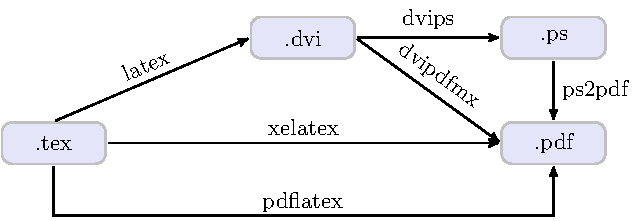
\includegraphics{pgf.pdf}
\caption{编译和格式转换}
\label{fig:compile}
\end{figure}

\section{语法和结构}\label{sec:structure}

\subsection{语法}

\LaTeX 源文件的语句可以分为三种:命令 (command) 、数据和注释 (comment) 。
命令又分为普通命令和环境 (environment) 。普通命令以 \verb|\| 起始,大多只有一行;而环境包含一对起始声明和结尾声明,一般用于多行内容的场合。命令和环境可以互相嵌套。数据就是普通内容。注释语句以 \verb|%| 起始,它在编译过程中被忽略。

比如在 \autoref{exa:helloworld} 中,第1行是注释,第2行是普通命令;第
3, 5行是环境的起始和结尾声明;第4行是数据。

\subsection{物理结构}

\LaTeX 文档的结构可以分为物理结构和逻辑结构。前者指的是源文件的组织形式,包括序言 (preamble) 和正文两部分;后者则是最终输出文档的结构,包括标题、目录、章节等。这里只简要介绍一些基本概念,在第十章还会展开详谈。

序言用来完成一些设置,比如指定文档类型,引入宏包,定义命令、环境等;文档的实际内容则放在正文部分。它们的基本用法如下:

\begin{Code}[]
\documentclass[options]{class}  %文档类声明
\usepackage[options]{package}   %引入宏包
...
\begin{document}                %正文
...
\end{document}
\end{Code}

常用的文档类 (documentclass) 有三种:\texttt{article, report, book},它们的基本选项见 \autoref{tab:class_options}。

\begin{table}[htbp]
\centering
\caption{文档类常用选项}
\label{tab:class_options}
\begin{tabularx}{350pt}{lX}
  \toprule
  10pt, 11pt, 12pt & 正文字号,缺省10pt。\LaTeX 会根据正文字号选择标题、上下标等的字号。\\
  letterpaper, a4paper & 纸张尺寸,缺省是 letterpaper。\\
  notitlepage, titlepage & 标题后是否另起新页。article 缺省 notitlepage,report 和 book 缺省有 titlepage。\\
  onecolumn, twocolumn & 栏数,缺省单栏。\\
  oneside, twoside & 单面双面。article 和 report 缺省用单面,book 缺省用双面。\\
  landscape & 横向打印,缺省是纵向。\\
  openany, openright & 此选项只用于 report 和 book。report 缺省 openany,book 缺省 openright。\\
  draft & 草稿模式。有时某些行排得过满,draft 模式可以在它们右边标上粗黑线提醒用户。\\
  \bottomrule
\end{tabularx}
\end{table}

\LaTeX 核心只提供基本功能,很多功能要通过宏包来实现。其他一些编程语言也有类似的模块化机制,比如 C/C++的 \texttt{include},Java 的 \texttt{import}。

\subsection{逻辑结构}

一份文档的开头通常有标题、作者、摘要等信息,之后是章节等层次结构,内容则散布于层次结构之间。文档比较长时我们还可以使用目录。

标题、作者、日期等命令用法如下,注意 \verb|\maketitle| 命令要放在最后。

\begin{Code}[]
\title{LaTeX Notes}
\author{Alpha Huang}
\date{\today}
\maketitle
\end{Code}

article和report可以有摘要,book里没有。摘要环境用法如下:

\begin{Code}[]
\begin{abstract}
...
\end{abstract}
\end{Code}

\LaTeX 提供了七种层次结构命令,每个高级层次可以包含若干低级层次。article 中没有 chapter,而 report 和 book 则支持所有层次。

\begin{example}[h]
\begin{Code}[numbers=left]
\part{...}          %Level -1
\chapter{...}       %Level 0
\section{...}       %Level 1
\subsection{...}    %Level 2
\subsubsection{...} %Level 3
\paragraph{...}     %Level 4
\subparagraph{...}  %Level 5
\end{Code}
\caption{层次结构}
\label{tab:structure}
\end{example}

我们可以用 \verb|\tableofcontents| 命令来生成目录。系统会自动设定目录包含的章节层次,用户也可以显式指定目录层次深度。比如下面的命令指定目录深度为2,也就是只显示 subsection 及以上层次的目录。注意设定目录深度命令要放在列目录命令的前面。

\begin{Code}[]
\setcounter{tocdepth}{2} %设定目录深度
\tableofcontents         %列出目录
\end{Code}

初次使用目录,或章节图表等层次结构发生变化时,都需要执行两遍编译命令才能获得正确结果。\LaTeX 之所以设计成这样是因为当时的电脑内存容量有限。

如果我们不想让某些层次的标题出现在目录里,则可以给 \autoref{tab:structure} 中的命令加上星号。

\begin{Code}[]
\chapter*{...}
\section*{...}
\subsection*{...}
\subsubsection*{...}
\end{Code}

类似地,我们也可以用下面的命令生成插图和表格目录,插图和表格功能将在后面相关章节中介绍。这两种目录也都需要编译两遍才能获得正确结果。

\begin{Code}[]
\listoffigures
\listoftables
\end{Code}

\section{文字}

文档的内容可以分为文本模式和数学模式。前者是缺省工作方式;要输入数学内容则需要特殊命令或环境。本章只涉及文本模式,第四章会介绍数学模式。

\subsection{字符输入}
\label{sec:char_input}

文档中可以输入的文字符号大致可以分为:普通字符、控制符、特殊符号、预定义字符串、注音符号等。

普通字符可以直接输入,而有些字符 (例如\~{} \# \$ \% \^{} \& \_ \{ \} 等) 被用作特殊的控制符,输入时多数需要在前面加个反斜杠 \verb|\| 来转义。而 \verb|\|本身则要用 \verb|\textbackslash| 命令来输入,因为 \verb|\\| 被用作换行指令\footnote{为什么不用 C 语言的 \verb|\n| 呢,也许因为 \TeX 的编程语言是 Pascal。}。

\begin{Code}[]
\~ \# \$ \% \^ \& \_ \{ \} \textbackslash
\end{Code}

\autoref{tab:symbols} 给出一些特殊符号和预定义字符串的输入方法;其中 \verb|\XeTeX|, \verb|\XeLaTeX| 命令需要 \texttt{metalogo} 宏包,\verb|\MF|, \verb|\MP| 命令需要 \texttt{mflogo} 宏包,\verb|\AmS| 命令需要 \texttt{texnames} 宏包。\autoref{tab:accent} 列出一些注音符号。更多的符号见 Scott Pakin\indexPakin{} \footnote{UIUC 计算机系 1995年硕士,2001年博士。现供职于洛斯阿莫斯国家实验室 (Los Alamos National Laboratory) 。} 的符号列表\citep{Pakin_comprehensive}。

\begin{table}[htbp]
\centering
\caption{特殊符号和预定义字符串}
\label{tab:symbols}
\begin{tabular}{llll}
  \toprule
  \multicolumn{2}{c}{特殊符号} & \multicolumn{2}{c}{预定义字符串} \\
  \cmidrule(lr){1-2} \cmidrule(lr){3-4}
  \textcopyright  & \verb|\textcopyright| & \today & \verb|\today| \\
  {\lmr\textregistered} & \verb|\textregistered|& \TeX  & \verb|\TeX| \\
  {\lmr\texttrademark} & \verb|\texttrademark| & \LaTeX  & \verb|\LaTeX| \\
  \textyen        & \verb|\textyen|       & \LaTeXe  & \verb|\LaTeXe| \\
  \texteuro       & \verb|\texteuro|      & \XeTeX  & \verb|\XeTeX| \\
  \pounds         & \verb|\pounds|        & \XeLaTeX  & \verb|\XeLaTeX| \\
  \dots           & \verb|\dots|          & \MF & \verb|\MF| \\
  \P              & \verb|\P|             & \MP & \verb|\MP| \\
  \S              & \verb|\S|             & \AmS & \verb|\AmS| \\
  \bottomrule
\end{tabular}
\end{table}

\begin{table}[htbp]
\centering
\caption{注音符号}
\label{tab:accent}
\lmr
\begin{tabular}{lp{40pt}lp{40pt}lp{40pt}lp{85pt}}
  \toprule
  \.{A} & \verb|\.{A}| & \"{A} & \verb|\"{A}| & 
    \={A} & \verb|\={A}| & \`{A} & \verb|\`{A}| \\
  \'{A} & \verb|\'{A}| & \^{A} & \verb|\^{A}| & 
    \v{A} & \verb|\v{A}| & \~{A} & \verb|\~{A}| \\
  \d{A} & \verb|\d{A}| & \b{A} & \verb|\b{A}| & 
    \r{A} & \verb|\r{A}| & \textcircled{A} & \verb|\textcircled{A}| \\
  \bottomrule
\end{tabular}
\rmfamily
\end{table}

\LaTeX 中有短划线 (hyphen) 、中划线 (en-dash) 和长划线 (em-dash) 。短划线又称连字符,用来连接单词;中划线用来连接数字,可以通过重复两次短划线得到;长划线类似于中文的破折号,重复三次短划线。为了便于比较,这里也给出数学模式的减号。

\begin{example}[!h]
\begin{RLDemo}[]
computer-aided\\
1840--2010\\
to be---or not to be\\
$1-1=0$
\end{RLDemo}
\caption{划线和减号}
\label{exa:dash}
\end{example}

\subsection{字体样式和大小}
\label{sec:font_style}

拉丁文字体主要有三大类:衬线字体 (roman, serif) 、无衬线字体 (sans serif) \footnote{Sans 这个词来源于法语,就是“没有”的意思。}和等宽字体 (monospace, typewriter) 。衬线字体笔画的边缘部分有些修饰,类似于中文的宋体、仿宋、楷体、魏体等。无衬线字体的笔画则是平滑的,类似于中文的黑体。

字体还可以有粗体 (bold) 、斜体 (italic) 、伪斜体 (oblique, slanted) 、小型大写字母 (small caps) 等修饰效果。\TeX 提供了介于正常字体和粗体之间的半粗体 (medium weight) 。斜体通常对原字体进行了重新设计,它修饰精细,多用于衬线字体;伪斜体基本上是把原字体倾斜,多用于无衬线字体,一般伪斜体看起来比斜体要宽一些。小型大写字母的形状和大写字母相同但尺寸较小,一般高度和小写字母相似。

每种字体样式包含很多种具体的字体,第三章会有关于字体更详细的介绍,包括中文字体的设置。字体常用样式命令见 \autoref{tab:font_style}。

\begin{table}[htbp]
\centering
\caption{字体样式}
\label{tab:font_style}
\begin{tabular}{llll}
  \toprule
  \textrm{roman} & \verb|\textrm{...}| & 
    \textbf{bold face} & \verb|\textbf{...}| \\
  \textsf{sans serif} & \verb|\textsf{...}| & 
    \textmd{medium weight} & \verb|\textmd{...}| \\
  \texttt{typewriter} & \verb|\texttt{...}| & 
    \textit{italic} & \verb|\textit{...}| \\
  \textsc{Small Caps} & \verb|\textsc{...}| & 
    \textsl{slanted} & \verb|\textsl{...}| \\
  \bottomrule
\end{tabular}
\end{table}

\LaTeX 的字体强调命令 \verb|\emph| 在不同字体环境中有不同的效果。如果周围文字是正体,它就是斜体;反之它就是正体。\verb|\underline| 命令可以给字体加下划线,但是它不能正确断字。 \texttt{ulem} 宏包改进了断字,还增加了波浪线和删除线等命令。只是 \texttt{ulem} 把 \verb|\emph| 重定义成了下划线,我们可以在引用宏包时加个选项改回去:\verb|\usepackage[normalem]{ulem}|。

\begin{example}[htbp]
\begin{RLDemo}[]
\emph{emphasis}\\
\uline{underline}\\
\uwave{waveline}\\
\sout{strike-out}
\end{RLDemo}
\caption{字体强调和下划线}
\end{example}

\LaTeX 会根据正文的字体大小来调整标题、章节、上下标、脚注等的字号。我们也可以用 \autoref{tab:fontsize} 中的命令来设置字体相对尺寸,比如正文的字号是10pt, 11pt, 12pt 时,tiny的字号就分别是5pt, 6pt, 6pt。

\begin{table}[htbp]
\centering
\caption{字体相对尺寸}
\label{tab:fontsize}
\begin{tabular}{llrrr}
  \toprule
  & & \multicolumn{3}{c}{正文字号} \\
  \cmidrule(lr){3-5}
  样本 & 命令 & 10pt & 11pt & 12pt \\
  \midrule
  \tiny{sample} & \verb|\tiny|         & 5pt  & 6pt  & 6pt \\
  \scriptsize{sample} & \verb|\scriptsize|   & 7pt  & 8pt  & 8pt \\
  \footnotesize{sample} & \verb|\footnotesize| & 8pt  & 9pt  & 10pt \\
  \small{sample} & \verb|\small|        & 9pt  & 10pt & 11pt \\
  \normalsize{sample} & \verb|\normalsize|   & 10pt & 11pt & 12pt \\
  \large{sample} & \verb|\large|        & 12pt & 12pt & 14pt \\
  \Large{sample} & \verb|\Large|        & 14pt & 14pt & 17pt \\
  \LARGE{sample} & \verb|\LARGE|        & 17pt & 17pt & 20pt \\
  \huge{sample} & \verb|\huge|         & 20pt & 20pt & 25pt \\
  \Huge{sample} & \verb|\Huge|         & 25pt & 25pt & 25pt \\
  \bottomrule
\end{tabular}
\end{table}

\subsection{换行、换页和断字}

通常 \LaTeX 会自动换行,我们也可以用 \verb|\\| 或 \verb|\newline| 命令来强制换行;用 \verb|\newpage| 命令来强制换页。

\LaTeX 也会自动断字 (hyphenate) ,使得每一行的字间距分布均匀。有时我们也需要显式指明断字位置,比如下例就指明 BASIC 这个词不能断开,而 blar-blar-blar 可以在-处断开。

\begin{Code}[]
\hyphenation{BASIC blar-blar-blar}
\end{Code}

\section{长度}
\label{sec:length}

为了精确排版,人们需要控制排版对象的尺寸和位置。\LaTeX 中常用长度单位见 \autoref{tab:unit},其中 point 是个传统印刷业采用的单位,而 big point 是 Adobe 推出 PostScript 时定义的新单位。em 是个相对单位,比如当前字体是 11pt 时,1em 就是 11pt;ex 和 mu 也是相对单位。

\begin{table}[htbp]
\caption{常用长度单位}
\label{tab:unit}
\centering
\begin{tabular}{llllll}
  \toprule
  in & 英寸 & pt & point, 1/72.27 in  & em & 当前字体中字母M的宽度 \\
  cm & 厘米 & bp & big point, 1/72 in & ex & 当前字体中字母x的高度 \\
  mm & 毫米 & pc & pica, 12 pt        & mu & math unit,1/18 em \\
  \bottomrule
\end{tabular}
\end{table}

\LaTeX 为排版对象的尺寸和位置定义了一系列宏变量,以便在排版时重用。我们可以用下面的方法来改变宏变量的值或定义新的宏变量,

\begin{Code}[]
\setlength{`变量名`}   %设置变量的值
\addtolength{`变量名`} %增加变量的值
\newlength{`变量名`}   %定义新变量
\end{Code}

\section{对齐和间距}

\subsection{段落对齐}

\LaTeX 中的段落缺省两端对齐 (fully justified) ,下面的三个环境可以让段落分别居左、居右或居中对齐。

另有三个命令 \verb|\raggedright|、\verb|\centering|、\verb|\raggedleft| 也可以完成同样功能。

\begin{example}[h]
\LoadFRLDemo[]{texlet/par-left}
\LoadFRLDemo[]{texlet/par-right}
\LoadFRLDemo[]{texlet/par-center}
\caption{段落对齐方式}
\end{example}

\subsection{缩进和段间距}
\label{sec:parskip}

\LaTeX 正文中第一个段落缺省不缩进首行,我们可以用 \texttt{indentfirst} 宏包使得第一段也缩进首行。段落首行缩进的距离可以用 \verb|\parindent| 变量来控制,段落之间的距离可以用 \verb|\parskip| 变量来控制。

\begin{Code}[]
\usepackage{indentfirst}
...
\setlength{\parindent}{2em}
\addtolength{\parskip}{3pt}
\end{Code}

\subsection{行间距}
行间距是段落中相邻两行基线之间的距离,\LaTeX 缺省使用单倍行距。我们可以用 \verb|\linespread| 命令来控制行距。

\begin{Code}[]
\linespread{1.3} %一倍半行距
\linespread{1.6} %双倍行距
\end{Code}

\verb|\linespread| 命令不仅会改变正文行距,同时也把目录、脚注、图表标题等的行距给改了。如果只想改正文行距,可以使用 \texttt{setspace} 宏包的行距命令 (见 \autoref{exa:setspace_cmd})。

\begin{example}[h]
\begin{Code}[]
\usepackage{setspace}
...
\singlespacing    %单倍行距
\onehalfspacing   %一倍半行距
\doublespacing    %双倍行距
\setstretch{1.25} %任意行距
\end{Code}
\caption{行距命令}
\label{exa:setspace_cmd}
\end{example}

上述行距命令对全文的行距都会产生影响,\texttt{setspace} 宏包还提供了 \texttt{singlespacing}, \texttt{onehalfspacing}, \texttt{doublespacing} 等环境,可以用来设置局部文字的行距(见 \autoref{exa:setspace_env})。

\begin{example}[h]
\begin{RLDemo}[]
\begin{doublespacing}
double\\spacing
\end{doublespacing}
\end{RLDemo}
\begin{RLDemo}[]
\begin{spacing}{1.25}
any\\spacing
\end{spacing}
\end{RLDemo}
\caption{行距环境}
\label{exa:setspace_env}
\end{example}

\section{特殊段落}
\subsection{摘录}

\LaTeX 中有三种摘录环境:\texttt{quote}, \texttt{quotation}, \texttt{verse}。 \texttt{quote} 两端都缩进, \texttt{quotation} 在 \texttt{quote} 的基础上增加了首行缩进,\texttt{verse} 比 \texttt{quote} 多了第二行起的缩进。

\begin{example}[h]
\LoadFRLDemo[]{texlet/quote-quote}
\LoadFRLDemo[]{texlet/quote-quotation}
\LoadFRLDemo[]{texlet/quote-verse}
\caption{摘录环境}
\end{example}

\subsection{原文打印}
文档中的命令和源代码通常使用等宽字体,也就是原文打印。正文间插入少量等宽文字可以使用 \verb|\verb| 命令;大段原文打印用 \texttt{verbatim} 环境比较方便,它的带星号版本可以标出空格。

\begin{example}[h]
\begin{RLDemo}[numbers=left]
\verb|command| 行间命令
\begin{verbatim}
printf("Hello, world!");
\end{verbatim}
\begin{verbatim*}
printf("Hello, world!");
\end{verbatim*}
\end{RLDemo}
\caption{原文打印}
\end{example}

Timothy van Zandt\indexVanZandt{} \footnote{宾州大学经济系1985年学士,1989年博士。1990年加入普林斯顿,1998年跳到欧洲工商管理学院。} 等人的 \texttt{fancyvrb} 宏包\citep{Zandt_fancyvrb}和 Brooks Moses\indexMoses{} \footnote{1997年弗吉尼亚理工学院机械学士,2007年斯坦福机械博士,毕业后加入一家软件公司源码巫师 (CodeSourcery) 。} 等人的 \texttt{listings} 宏包\citep{Moses_listings}提供了更多的原文打印功能,比如行号、边框、背景、语法着色等。

\subsection{脚注}

脚注可以使用 \verb|\footnote| 命令;如要改变脚注编号形式,可以使用以下命令。
在 \autoref{exa:footnote} 中,\verb|footnote| 是一个计数器 (counter) ;计数器有五种显示格式 (见 \autoref{tab:counter_format}) ,重定义 \verb|\thefootnote| 宏时可任选。

\begin{example}[h]
\LoadFRLDemo[]{texlet/note-footnote}
\begin{Code}[numbers=left]
\renewcommand{\thefootnote}{\roman{footnote}} %i, ii, iii
\end{Code}
\caption{脚注}
\label{exa:footnote}
\end{example}

以后我们还会遇到其他一些计数器,都可以用重定义 \verb|\thecounter| 的方法改变它们的显示格式。

\begin{table}
\centering
\caption{计数器显示格式}
\label{tab:counter_format}
\begin{tabular}{lll}
  \toprule
  阿拉伯数字 & \verb|\arabic{counter}| & 1, 2, 3\dots \\
  小写英文字母 & \verb|\alph{counter}| & a, b, c\dots \\
  大写英文字母 & \verb|\Alph{counter}| & A, B, C\dots \\
  小写罗马数字 & \verb|\roman{counter}| & i, ii, iii\dots \\
  大写罗马数字 & \verb|\Roman{counter}| & I, II, III\dots \\
  \bottomrule
\end{tabular}
\end{table}

原始的脚注命令不能包含原文打印命令或环境,我们可以用 \verb|\texttt| 命令来输入等宽字体,或者用 \texttt{fancyvrb} 宏包的 \verb|\VerbatimFootnotes| 命令重定义 \verb|\footnote| 命令。

\subsection{边注}

边注可以使用 \verb|\marginpar| 命令。单面排版时,边注缺省排在页面右边空白处;双面排版时,边注在外侧,也就是左页的左边或右页的右边;双栏页面的边注排在最近的页边。如要切换边注的方向,可以使用 \verb|\reversemarginpar| 和 \verb|\normalmarginpar| 命令。

\verb|\marginpar| 命令使用浮动体 (float) \footnote{浮动体详见第五章插图和第九章表格。} 来生成边注,所以不能在其他浮动体或脚注内嵌套。 \texttt{marginnote} 宏包的 \verb|\marginnote| 命令不使用浮动体,因而没有这个缺陷。

\begin{example}[h]
\marginnote{正常边注}
\reversemarginpar
\marginnote{反向边注}
\normalmarginpar

\begin{Code}[]
\marginnote{`正常边注`}
\reversemarginpar
\marginnote{`反向边注`}
\normalmarginpar
\end{Code}
\caption{边注}
\end{example}

\subsection{注释}
前面提到可以用百分号来标明注释,但是对于大段文字的注释,百分号就显得比较繁琐 \footnote{有的编辑器提供切换多行百分号的功能,比如TeXNicCenter。}。这时我们可以使用 \texttt{verbatim} 宏包的 \texttt{comment} 环境。

\begin{Code}[]
\begin{comment}
...
\end{comment}
\end{Code}

\section{列表}\label{sec:list}

\subsection{基本列表}

\LaTeX 有三种基本列表环境:无序列表、有序列表、描述列表。这些列表可以单独使用,也可以互相嵌套。

\begin{example}[h]
\subfloat[无序列表]{%
\makebox[\textwidth][l]{%
\LoadRLDemo[numbers=left]{texlet/list-itemize}%
}}\\
\subfloat[有序列表]{%
\makebox[\textwidth][l]{%
\LoadRLDemo[numbers=left]{texlet/list-enumerate}%
}}\\
\subfloat[描述列表]{%
\makebox[\textwidth][l]{%
\LoadRLDemo[numbers=left]{texlet/list-description}%
}}
\caption{基本列表}
\end{example}

\subsection{其他列表}

上述列表的缺省行间距较大,如要节省空间,可以考虑 Bernd Schandl\indexSchandl{}\footnote{1997年凯撒斯劳腾工业大学 (Kaiserslautern University of Technology) 数学硕士,1999年克莱姆森大学数学博士。} 的 \texttt{paralist} 宏包,它提供了一系列压缩列表和行间列表环境。

\begin{example}[!h]
\begin{RLDemo}[numbers=left]
\begin{compactitem}
  \item C++
  \item Java 
  \item HTML
\end{compactitem}
\end{RLDemo}
\begin{RLDemo}[numbers=left]
\begin{compactenum}
  \item C++
  \item Java 
  \item HTML
\end{compactenum}
\end{RLDemo}
\begin{RLDemo}[numbers=left]
\begin{compactdesc}
  \item[C++] 编程语言,
  \item[Java] 编程语言,
  \item[HTML] 标记语言。
\end{compactdesc}
\end{RLDemo}
\caption{压缩列表}
\label{exa:compact_list}
\end{example}

\begin{example}[!h]
\begin{RLDemo}[numbers=left]
\begin{inparaitem}
  \item C++
  \item Java 
  \item HTML
\end{inparaitem}
\end{RLDemo}
\begin{RLDemo}[numbers=left]
\begin{inparaenum}
  \item C++
  \item Java 
  \item HTML
\end{inparaenum}
\end{RLDemo}
\begin{RLDemo}[numbers=left]
\begin{inparadesc}
  \item[C++] 编程语言,
  \item[Java] 编程语言,
  \item[HTML] 标记语言。
\end{inparadesc}
\end{RLDemo}
\caption{行间列表}
\label{exa:inline_list}
\end{example}

%\clearpage
\subsection{定制列表}

如要改变无序列表的列表符号和有序列表的编号形式,可以使用以下代码,其效果见 \autoref{exa:customized_list}。

\begin{Code}[]
\renewcommand{\labelitemi}{-}
\renewcommand{\theenumi}{\alph{enumi}}
\end{Code}

\renewcommand{\labelitemi}{-}
\renewcommand{\theenumi}{\alph{enumi}}

\begin{example}[htbp]
\LoadRLDemo[numbers=left]{texlet/list-itemize}\\
\LoadRLDemo[numbers=left]{texlet/list-enumerate}
\caption{定制列表}
\label{exa:customized_list}
\end{example}

\renewcommand{\labelitemi}{\ensuremath{\bullet}}
\renewcommand{\theenumi}{\arabic{enumi}}

\section{盒子}
\label{sec:box}

\LaTeX 在排版时把每个对象 (小到一个字母,大到一个段落) 都视为一个矩形盒子 (box) ,我们在HTML和CSS中也可以见到类似的模型。

\subsection{初级盒子}

最简单的盒子命令是 \verb|\mbox|和 \verb|\fbox|。前者把一组对象组合起来,后者在此基础上加了个边框。

\begin{example}[htbp]
\begin{RLDemo}[]
\mbox{010 6278 5001}
\fbox{010 6278 5001}
\end{RLDemo}
\caption{ \texttt{mbox}和 \texttt{fbox}}
\label{exa:mbox}
\end{example}

\subsection{中级盒子}

稍复杂的 \verb|\makebox| 和 \verb|\framebox| 命令提供了宽度和对齐方式控制的选项。其对齐方式有居中 (缺省) 、居左、居右和分散对齐,分别用 \texttt{c}, \texttt{l}, \texttt{r}, \texttt{s} 来表示。

\begin{example}[htbp]
\LoadFRLDemo[]{texlet/box-make}
\caption{ \texttt{makebox}和 \texttt{framebox}}
\label{exa:makebox}
\end{example}

\subsection{高级盒子}

大一些的对象比如整个段落可以用 \verb|\parbox| 命令或 \texttt{minipage} 环境,两者语法类似,有宽度、高度、外部对齐、内部对齐等选项。这里的外部对齐是指该盒子与周围对象的纵向关系,有三种方式:居顶、居中和居底对齐,分别用 \texttt{t}, \texttt{c}, \texttt{b} 来表示。内部对齐是指该盒子内部内容的纵向排列方式,也是同样三种。

\verb|语法:[外部对齐][高度][内部对齐]{宽度}{内容}|

\begin{example}[htbp]
\LoadCode[numbers=left]{texlet/box-par-esc}
\input{texlet/box-par}
\caption{\texttt{parbox} 和 \texttt{minipage}}
\label{exa:parbox}
\end{example}

%\subsection{彩色盒子}
%\subsection{盒子升降}
%\subsection{盒子存取}

\section{交叉引用}
\label{sec:crossref}

在 \LaTeX 中我们可以任意设置标签,然后引用标签前面最近一个对象 (章、节、图、表等) 的编号或者页码,这就是交叉引用 (cross reference) 。\autoref{exa:ref} 中的 \texttt{marker} 是一个标签名,它在全文中须保持唯一。

\begin{example}[h]
\LoadFBTDemo[]{texlet/ref}% label in example environment doesn't work
\caption{交叉引用}
\label{exa:ref}
\end{example}

文档中新增标签后,第一次编译时会得到类似下面的警告信息。因为第一次编译只会扫描出有标签的地方,第二次编译才能得到正确结果。

\begin{Code}[]
LaTeX Warning: There were undefined references.
LaTeX Warning: Label(s) may have changed. Rerun to get cross-references right.
\end{Code}

\bibliographystyle{unsrtnat}
\bibliography{lnotes2}

\chapter{字体}

英文中的 typeface 和 font 一般都被翻译为字体,传统印刷业通常使用 typeface,电脑字体通常使用 font;当然也有很多人混用这两个词。包老师认为电脑字体的诸多相关概念可以划分为三个层次:

\begin{compactenum}
  \item 编码层,字符 (包括字母、数字、符号、控制码等) 的索引和编码,也就是字符集 (character set) 和字符编码 (character encoding) 。
  \item 格式层,字形 (glyph) 的定义描述方法,以及字体的文件存储格式。
  \item 显示层,字体的外在表现形式,比如字体的样式,或具体的字体。
\end{compactenum}

看到这里好奇的读者可能会问,为什么微软\indexMSFT{} Word 和其他所见即所得软件可以直接用下拉菜单设置字体,同样是标记语言的HTML也可以方便地设置字体,而 \LaTeX 就要牵扯这么多概念?我们不得不承认,这是 \LaTeX 的历史局限性之一。Knuth\indexKnuth 当初设计 \TeX 时,既没有 Unicode 字符集和 UTF-8 编码,也没有 TrueType 和 OpenType 字体格式。

包老师语重心长地说,道路是曲折的,前途是光明的。这不马上就要侃到 \XeTeX 了,这些困难只是黎明前的黑暗。

\section{字符集和编码}
\label{sec:encoding}

众所周知电脑内部采用二进制编码,因为它易于用电子电路实现。所有字符在电脑内部都是用二进制表示的,字符集的二进制编码被称为字符编码,有时人们也会混用这两个术语。

1963年ANSI\indexANSI 发布了基于电报码的 ASCII,这就是最早的字符编码,它用7位 (bit) 表示了$2^7=128$个字符,只能勉强覆盖英文字符。

美国人发明了电脑,他们优先考虑英语是可以理解的。后来随着电脑技术的传播,人们呼吁把字符编码扩充到8位也就是一个字节 (byte) ,可以涵盖$2^8=256$个字符。

于是ISO\indexISO 在1980年代中期推出了 ISO 8859,256个字符显然也不能满足需要,所以8859被分为十几个部分:从8859-1 (西欧语言) 、8859-2 (中欧语言) ,直到8859-16 (东南欧语言) ,覆盖了大部分使用拉丁字母的语言文字。

在 ISO 标准完全定型之前,IBM 就有一系列自己的字符编码,也就是代码页 (code page) ,比如437 (扩展ASCII) 、850 (西欧语言) 、852 (东欧语言) 。IBM\indexIBM 代码页通常被用于控制台 (console) 环境,也就是 MS-DOS 或 Unix Shell 那样的命令行环境。

微软\indexMSFT 将 IBM 代码页称为 OEM 代码页,自己定义的称为 ANSI 代码页,比如1252 (西欧语言), 1250 (东欧语言), 936 (GBK简体中文), 950 (Big5繁体中文), 932 (SJIS日文), 949 (EUC-KR韩文) 等。

1981年,中国大陆推出了第一个自己的字符集标准 GB2312,它是一个94×94的表,包括7445个字符。GB2312 通常采用双字节的 EUC-CN 编码,所以后者也常常被称为 GB2312编码;其实 GB2312 还有另一种编码方式HZ,只是不常用。

GB2312 中没有朱镕基的“镕”字,于是它在1993年被扩展为 GBK,包含21886个字符。GBK 不是正式标准。2000年发布的 GB18030 包含70244个字符,采用四字节编码。GB18030 之前还出现过一个 GB13000,但是没有形成气候。

1990年 ISO 推出了通用字符集 (universal character set,UCS) ,即 ISO 10646,意图一统江湖。它的容量是一百多万个字符,目前实际使用的有十万个左右。UCS 有两种编码:双字节的 UCS-2 和四字节的 UCS-4。

ISO 之外还有个希望一统江湖的组织:统一码联盟 (The Unicode Consortium)\indexUnicode ,它于1991 年推出了 Unicode 1.0。后来两家组织意识到没必要做重复工作,于是双方开始合并成果,携手奔小康。Unicode 从2.0版开始采用与 ISO 10646-1 相同的编码。

Unicode 主要有三种编码:UTF-8, UTF-16, UTF-32。UTF-8 使用一至四个8位编码。UTF-16 用一或两个16位编码,基本上是 UCS-2 的超集,和 ASCII 不兼容。UTF-32 用一个32位编码,它是 UCS-4 的一个子集。

IETF\indexIETF 要求所有网络协议都支持 UTF-8,互联网电子邮件联盟 (Internet Mail Consortium, IMC)\indexIMC 也建议所有电子邮件软件都支持 UTF-8,所以它已成为互联网上的事实标准。

\section{字体格式}

\subsection{点阵和矢量字体}

电脑字体的数据格式可以分为三大类:点阵 (bitmap) 字体、轮廓 (outline) 字体和笔画 (stroke-based) 字体。

点阵字体通过点阵来描述字形。早期的电脑受到容量和绘图速度的限制,多采用点阵字体。点阵字体后来渐渐被轮廓字体所取代,但是很多小字号字体仍然使用它,因为这种情况下轮廓字体缩放太多会导致笔画不清晰。

轮廓字体又称作矢量字体,它通过一组直线段和曲线来描述字形。轮廓字体易于通过数学函数进行缩放等变换,形成平滑的轮廓。轮廓字体的主要缺陷在于它所采用的贝塞尔曲线 (Bézier curves) 在光栅设备 (比如显示器和打印机) 上不能精确渲染,因而需要额外的补偿处理比如字体微调 (font hinting) 。但是随着电脑硬件的发展,人们一般不在意它比点阵字体多出的处理时间。

笔画字体其实也是轮廓字体,不过它描述的不是完整的字形,而是笔画。它多用于东亚文字。

\subsection{常见字体格式}

当前常见的轮廓字体格式有:Type 1, TrueType, OpenType。

1984年 Adobe\indexAdobe 推出PostScript时,同时支持两种字体格式:Type 1 和 Type 3,它们都采用三次贝塞尔曲线。Type 1 支持微调,它使用一个简化的 PostScript 子集;Type 3 不支持微调,但它可以使用全部 PostScript 功能,因此既可包含轮廓字体也可包含点阵字体信息。

1991年 苹果\indexApple 发布了 TrueType,它采用二次贝塞尔曲线。二次曲线处理起来比三次曲线快,但是需要更多的点来描述。所以从 TrueType 到 Type 1 的转换是无损的,反之是有损的。1994年苹果开始研究 TrueType 的下一代技术:TrueType GX,它后来演变为 Apple advanced typography (AAT) 。

1996年微软和 Adobe 联合发布了 OpenType,它可以被认为是 Type 1 和 TrueType 的超集,既可使用二次曲线,也可使用三次曲线。它比起 TrueType 和 AAT 的优势还有:平台独立、开放、易于开发,并且支持更多的语言比如阿拉伯语。

早在1984年 Knuth 就发布了 \MF ,它与 TrueType 和 OpenType 的区别是,不直接描述字形轮廓,而描述生成轮廓的笔的轨迹。笔的形状可以是椭圆形或多边形,尺寸缩放自如,字形边缘也柔和一些。两种字体可以用同一个 \MF 文件,当然还有不同的参数。\MF 技术如此先进,却没有流行开来。对此 Knuth 解释道,要求一位设计字体的艺术家掌握60个参数太变态了,那是用来折磨数学家的。

Type 1 和 Type 3 把字体的尺寸 (metrics) 信息和字形 (glyph) 信息分别存储。字体尺寸文件有两种:AFM (Adobe font metrics) 和 PFM (printer font metrics),字形文件也有两种:PFA (printer font ASCII) 和 PFB (printer font binary) 。\LaTeX 使用的尺寸格式是 TFM (TeX font metrics) 。

TrueType 和 OpenType 则将字体数据都存在一个文件里,它们的文件后缀分别是是.ttf和.otf。\MF 虽然用矢量图形来定义字形,实际输出的却是一种点阵格式:PK (packed raster) 。

这些字体格式按照技术先进性,从高到低依次为:OpenType, TrueType, Type 1, Type 3, PK,所以我们要优先选用 OpenType 和 TrueType。

PostScript 文件可以包含 Type 1 和 Type 3 字体,而 PDF 除了这两种还支持 TrueType 和 OpenType 字体。

\subsection{合纵连横}

当年 Adobe\indexAdobe{}推出 Type 1 和 Type 3 时,前者收费,后者是公开的自由规范。Type 1 专利许可费十分昂贵,穷人们只好用免费的 Type 3。为了打破这种垄断,苹果开发了 TrueType。1991年 TrueType 发布之后,Adobe 随即公开了 Type 1 的规范,它从贵族堕落为平民,因而流行开来。

1980年代中后期,Adobe 的大部分盈利来自于 PostScript 解释器的许可费。面对这种垄断局面,微软和苹果联合了起来。微软把买来的 PostScript 解释器 TrueImage 授权给苹果,苹果则把 TrueType 授权给微软。

微软得陇望蜀,又企图获得 AAT 的许可证,未遂。为了打破苹果的垄断,微软联合 Adobe 在1996年发布了 OpenType。Adobe 在2002年末将其字体库全面转向 OpenType。

上面这几出精彩好戏充分展示了商场上的勾心斗角、尔虞我诈,没有永恒的伙伴,只有永恒的利益。但它同时也告诉我们,市场竞争中受益的还是广大的消费者。

\section{常见字体}

在 \ref{sec:font_style} 小节中我们提到每种字体样式可以包含很多种具体的字体。为了方便读者,\autoref{tab:font} 列出一些最常见的字体。\TeX 的缺省字体是 Knuth 用 \MF 生成的 Computer Modern;\XeTeX 的缺省字体是1997年 \AmS 发布的 Latin Modern,它基于 Computer Modern,但是扩展了其字符集,其封装格式有 Type 1 和 OpenType。

\begin{table}[htbp]
\caption{常见字体}
\label{tab:font}
\centering
\begin{tabular}{llll}
  \toprule
  操作系统 & 衬线字体        & 无衬线字体 & 等宽字体 \\
  \midrule
  \multirow{3}{*}{Windows}
    & Times New Roman & Tahoma     & Courier New \\
    & Georgia         & Verdana    & Lucida Console \\
    & Palatino Linotype & Arial    & Consolas \\
  \midrule
  \multirow{3}{*}{macOS}
    & Times           & Helvetica  & Monaco \\
    & Georgia         & Lucida Grande & Courier \\
    & Times New Roman & Geneva     & Courier New \\
  \bottomrule
\end{tabular}
\end{table}

\section{字体的应用}

从理论上讲,任何电脑字体只要有TFM,\TeX 就可以使用它。然而早期的 \TeX 只能使用 \MF 生成的字体。直到 \LaTeXe 时代 NFSS 出现后,Type 1 和 Type 3 才在 \LaTeX 中得到广泛应用。后起之秀 \XeTeX 则极大程度地简化了 TrueType 和 OpenType 的配置,而且它还支持 Unicode。

\texttt{latex}, \texttt{pdflatex}, \texttt{xelatex} 编译程序,\texttt{dvips} 和 \texttt{dvipdfmx} 驱动,DVI 阅读器等分别采用不同的字体技术路线。本文主推 \XeLaTeX ,对其他早期技术只作简要介绍,聊以忆苦思甜。

\subsection{早期技术}

\subsubsection{latex和DVI}

我们用 \texttt{latex} 生成 DVI 时只需要 TFM 文件,因为 DVI 并不包含字形信息,而只包含对字体的引用。DVI 阅读器显示 DVI 时一般使用 PK,它在系统中查找相应的 \texttt{.pk} 文件,若找不到就调用 \MF 在后台自动生成。

\subsubsection{dvips}

缺省情况下,\texttt{dvips} 也会查找 \texttt{.pk},或调用 \MF 自动生成;然后把 PK 转换成包含点阵字体的 Type 3,它的参数 \texttt{-D} 可以用来控制该点阵字体的分辨率。用 \texttt{ps2pdf} 处理含 Type 3 的 PostScript 时,输出的自然是含 Type 3 的 PDF。

GSview\footnote{该软件已经停止更新,包老师正在寻找替代品。} 在低分辨率下可以很好地渲染 Type 3,Adobe Reader 或 Acrobat 却不能,因为它们使用的 Adobe Type Manager 不支持包含完整 PostScript 的 Type 3。因此含 Type 3 的 PDF 看起来会有些模糊,所以应尽量避免使用。

\texttt{dvips} 的另一个参数 \texttt{-Ppdf} 把 Type 1 嵌入生成的 PostScript,这样再 \texttt{ps2pdf} 就能生成含 Type 1 的 PDF。

\texttt{dvips} 不支持真正的 (native) TrueType,用户只能把 TrueType 先转成 PK 或 Type 1,这样绕了个弯效果总会打些折扣。

\texttt{dvips} 的字体详细使用方法可查阅其手册\citep{Rokicki_dvips}第六章,此处不赘述。

\subsubsection{dvipdfm(x)和pdflatex}

\texttt{dvipdfm} 支持 PK 和 Type 1,它可以用一个 \texttt{t1fonts.map} 文件建立 PK 文件和 Type 1 文件之间的映射,这样生成的 PDF 用的就是 Type 1。\texttt{dvipdfm} 也不支持真正的 TrueType。\texttt{dvipdfmx} 通过正确的设置可以使用真正的 TrueType,它对中日韩等东亚文字的支持也较好;只是其安装配置较繁琐,此处不赘述,实在有兴趣考古的读者可以参考 lnotes 第一版\citep{Huang_lnotes}。

pdflatex 支持 Type 1, TrueType,也在一定程度上支持 OpenType。它的配置也很繁琐,可以参考其用户手册\citep{Han_pdftex}第五章。

\subsection{XeTeX}

\XeTeX 可以直接使用电脑系统字体,不再需要 TFM 文件。我们首先需要知道电脑上有哪些字体,\XeTeX 用一个XML文件记录系统字体路径,MikTeX 用的是 \texttt{localfonts.conf},TeXlive 用的是 \texttt{fonts.conf}。

我们设置字体时需要字体的引用名,它和字体的文件名是不同的概念。\texttt{fc-list} 程序可以用来获取字体引用名,比如下面命令生成的文件 \texttt{myfonts.txt} 就是一份字体引用名列表。

\begin{Code}[]
fc-list > myfonts.txt
\end{Code}

带 \XeTeX 的发行包首次安装时会自动扫描这些字体目录,生成字体的缓存 (cache) 。每次系统安装了新字体时,我们需要手工运行字体缓存命令 \texttt{fc-cache},生成新的缓存。

\begin{Code}[]
fc-cache -r
\end{Code}

关于字体路径,\texttt{fc-list} 和 \texttt{fc-cache} 命令等的详细信息,可以参考 Michel Goossens (1951--)\indexGoossens{} \footnote{布鲁塞尔自由大学 (Free University of Brussels) 物理系1972年学士,1978年博士。1979年加入 CERN。合著\emph{\LaTeX{} Companion}, \emph{\LaTeX{} Graphics Companion}, \emph{\LaTeX{} Web Companion}等书。曾任TUG总统。} 编辑的\emph{\XeTeX{} Companion}\citep{Goossens_xetex}。

\XeTeX 提供的字体命令比较原始、繁琐,Will Robertson (1981--)\indexRobertson{} \footnote{阿德雷德大学 (University of Adelaide) 机械系2002年学士,2013年博士生,2016年讲师。} 的 \texttt{fontspec} 宏包提供了较好的封装。\XeLaTeX 下字体常用设置方法如下,详细信息可以参考 \texttt{fontspec} 的用户手册\citep{Robertson_fontspec}。

\begin{example}[h]
\begin{Code}[]
\usepackage{fontspec}
\setmainfont[Mapping=tex-text]{Times New Roman}
\setsansfont[Mapping=tex-text]{Tahoma}
\setmonofont{Courier New}
\end{Code}
\caption{\XeLaTeX 字体设置}
\label{exa:xelatex_font}
\end{example}

\autoref{exa:xelatex_font} 中的代码分别设置了衬线、无衬线和等宽字体样式对应的字体。在 \ref{sec:char_input} 小节 \autoref{exa:dash} 中我们学过中划线和破折号可以用 \texttt{--} 和 \texttt{---} 来输入。\TeX 中几个短划线是相连的,\XeTeX 中缺省它们之间是有空隙的。\autoref{exa:xelatex_font} 用 \texttt{Mapping} 参数指示改回 \TeX 的方式,即去掉短划线之间的空隙。

\section{中文解决方案}

\LaTeX 对中文的支持主要有两种方法:张林波\indexZhangLinbo{} \footnote{中科院数学与系统科学研究院研究员。} 的 CCT 和 Werner Lemberg (1968--)\indexLemberg{} \footnote{从维也纳音乐和表演艺术大学 (University of Music and Performing Arts, Vienna) 获得作曲、指挥、钢琴、乐团管理、歌手教练等五个专业文凭,后自学中文和数学。曾任职于奥地利和德国多家剧院和乐团,现任德国科布伦茨某剧院指挥。} 的 CJK 宏包。早期 CCT 比较流行,CJK 后来居上;新版 CCT 也可以和 CJK 配合使用。

支持简体中文的 \LaTeX 发行版有吴凌云等人的 CTeX 和李树钧\indexLiShujun{} \footnote{西安交大电子系1997年学士,2003年博士。2003年香港城市大学博士后,2005年香港理工大学博士后,2007年哈根函授大学 (Distance University of Hagen) 研究员,2008年康斯坦茨大学 (University of Konstanz) 研究员。} 的 ChinaTeX,支持繁体中文的有吴聪敏 (1952--)\indexWuCongmin{} \footnote{台湾大学电机学士,罗彻斯特大学经济学博士,台湾大学经济系教授。}、吴聪慧\indexWuConghui{} \footnote{新泽西理工学院电脑硕士,嘉南药理科技大学医务管理系助理教授。} 兄弟和翁鸿翎\indexWongHongling 的 cwTeX,蔡奇伟\indexCaiQiwei{} \footnote{犹他电脑博士,静宜大学资讯工程系副教授。} 的 PUTeX。这两个繁体中文的发行版本人都不熟悉,前两个简体中文发行版都包含MikTeX, CCT, CJK, WinEdt 等。

\XeTeX 问世后,孙文昌 (1970--)\indexSunWenchang{} \footnote{南开大学数学系1993年学士,1998年博士,毕业后留校作博士后,2000年副教授,2002年教授。} 推出了 \texttt{xeCJK} 宏包,用于排版中日韩等文字,包括字体选择,标点、文字间距调整等功能。它可以被认为是 CCT 和 CJK 在某种程度上的结合。

在 \autoref{exa:xecjk} 中引用宏包时,\texttt{CJKchecksingle} 参数防止段落最后一行只有一个汉字;\texttt{CJKnumber} 参数自动载入另一个宏包 \texttt{CJKnumber},它提供的 \verb|\CJKnumber| 命令可以把阿拉伯数字转换为中文数字。

\verb|\setCJKmainfont| 命令设置了中文正文字体,其参数 \texttt{BoldFont} 和 \texttt{ItalicFont} 分别设置粗体和斜体样式对应的字体。\verb|\setCJKsansfont|, \verb|\setCJKmonofont| 命令分别设置了无衬线和等宽字体样式对应的字体。

\begin{example}[h]
\begin{Code}[numbers=left]
\usepackage[CJKchecksingle,CJKnumber]{xeCJK}
\setCJKmainfont[BoldFont={Adobe Heiti Std}, 
  ItalicFont={Adobe Kaiti Std}]{Adobe Song Std}
\setCJKsansfont{Adobe Heiti Std}
\setCJKmonofont{Adobe Fangsong Std}
\punctstyle{hangmobanjiao}
\end{Code}
\caption{xeCJK}
\label{exa:xecjk}
\end{example}

其实严格地讲中文字体并没有衬线、无衬线、等宽、斜体等概念,只是习惯上宋体用得最多,辅以黑体、仿宋、楷体,文档会显得疏落有致,不至于太沉闷。如果我们把 \autoref{exa:xelatex_font} 和 \autoref{exa:xecjk} 中的命令结合起来,就可以为中英文分别设置字体。

xeCJK 宏包的详细用法可参考其用户手册\citep{Sun_xecjk}。另外 Yin Dian 的 zhspacing 宏包也可以完成类似功能,具体用法可参考其文档\citep{Yin_zhspacing}。

C\TeX 开发小组的 C\TeX 宏集是一个面向中文排版的通用 \LaTeX 排版框架,汉字输出支持、标点压缩、字体字号命令、标题文字汉化、中文版式调整、数字日期转换等支持功能,可适应论文、报告、书籍、幻灯片等不同类型的中文文档。包老师最近 (2019年) 才开始试用,读者请参考其手册\citep{CTeX_ctex}。

\bibliographystyle{unsrtnat}
\bibliography{lnotes2}

\chapter{数学}

\begin{quotation}
今有上禾三秉,中禾二秉,下禾一秉,实三十九斗;上禾二秉,中禾三秉,下禾一秉,实三十四斗;上禾一秉,中禾二秉,下禾三秉,实二十六斗。问上、中、下禾实一秉各几何?
\begin{gather*}
\begin{split}
  3x+2y+z &= 39 \\
  2x+3y+z &= 34 \\
  x+2y+3z &= 26 \\
\end{split}
\end{gather*}
\begin{flushright}
--- 《九章算术》
\end{flushright}
\end{quotation}

为了使用 \AmSLaTeX 提供的数学功能,我们需要在文档的序言部分加载 \texttt{amsmath} 宏包,其详细用法可参阅其用户手册\citep{AMS_amsmath}。更全面的数学内容排版可参阅 George Grätzer\indexGratzer{} \footnote{匈牙利厄特沃什·罗兰大学 (Eötvös Loránd University) 1960年数学博士,John von Neumann 的校友。现任加拿大曼尼托巴大学 (University of Manitoba) 教授。} 的 \emph{More Math into \LaTeX}\citep{Gratzer_more_math}。

\begin{Code}[]
\usepackage{amsmath}
\end{Code}

\section{数学模式}

\LaTeX 的数学模式有两种形式:行间 (inline) 模式和独立 (display) 模式。前者是指在正文中插入数学内容;后者独立排列,可以有或没有编号。简单数学公式的输入方法见 \autoref{tab:simplemath}。

\begin{table}[htbp]
\caption{简单数学公式的输入}
\label{tab:simplemath}
\centering
\begin{tabular}{ccccc}
  \toprule
  & \TeX 命令  & \LaTeX 命令    & \LaTeX 环境    & \texttt{amsmath} 环境\\
  \midrule
  行间公式      & \verb|$...$|   & \verb|\(...\)| & \texttt{math} & \\
  无编号独立公式 & \verb|$$...$$| & \verb|\[...\]| & \texttt{displaymath} & 
    \texttt{equation*}\\
  有编号独立公式 & & & \texttt{equation} & \texttt{equation} \\
  \bottomrule
\end{tabular}
\end{table}

行间公式和无编号独立公式都有多种输入方法,新手也许会看花了眼。懒人包老师的秘诀是用最短的:行间公式用 \verb|$...$|,无编号独立公式用 \verb|\[...\]|。建议不要用 \verb|$$...$$|,因为它和 \AmSLaTeX 有冲突。\texttt{ams\-math} 版本的 \texttt{equation} 环境可以嵌入次环境 (见 \ref{sec:longeq} 节) 。

\ref{sec:box} 节提到的 \verb|\fbox| 命令可以给文本内容加个方框,数学模式下也有个类似的命令 \verb|\boxed|。

\begin{example}[h]
\begin{RLDemo}[numbers=left]
Einstein's $E=mc^2$
\[ E=mc^2 \]
\[ \boxed{E=mc^2} \]
\begin{equation} 
  E=mc^2 
\end{equation}
\end{RLDemo}
\caption{数学模式}
\end{example}

\section{基本元素}

\subsection{希腊字母}

英文字母在数学模式下可以直接输入,希腊字母则需要用 \autoref{tab:greek} 中的命令输入,注意大写希腊字母的命令首字母也是大写。

\begin{table}[htbp]
\caption{希腊字母}
\label{tab:greek}
\centering
\begin{tabular}{llllllll}
  \toprule
  $\alpha$      & \verb|\alpha|      & $\theta$    & \verb|\theta|    & 
    $o$         & \verb|o|        & $\tau$     & \verb|\tau| \\
  $\beta$       & \verb|\beta|       & $\vartheta$ & \verb|\vartheta| & 
    $\pi$       & \verb|\pi|      & $\upsilon$ & \verb|\upsilon| \\
  $\gamma$      & \verb|\gamma|      & $\iota$     & \verb|\iota|     & 
    $\varpi$    & \verb|\varpi|   & $\phi$     & \verb|\phi| \\
  $\delta$      & \verb|\delta|      & $\kappa$    & \verb|\kappa|    & 
    $\rho$      & \verb|\rho|     & $\varphi$  & \verb|\varphi| \\
  $\epsilon$    & \verb|\epsilon|    & $\lambda$   & \verb|\lambda|   & 
    $\varrho$   & \verb|\varrho|  & $\chi$     & \verb|\chi| \\
  $\varepsilon$ & \verb|\varepsilon| & $\mu$       & \verb|\mu|       & 
    $\sigma$    & \verb|\sigma|   & $\psi$     & \verb|\psi| \\
  $\zeta$       & \verb|\zeta|       & $\nu$       & \verb|\nu|       & 
    $\varsigma$ & \verb|\varsigma|   & $\omega$   & \verb|\omega| \\
  $\eta$        & \verb|\eta|        & $\xi$       & \verb|\xi|       & 
    &                 &            & \\
  $\Gamma$      & \verb|\Gamma|      & $\Lambda$   & \verb|\Lambda|   & 
    $\Sigma$    & \verb|\Sigma|   & $\Psi$     & \verb|\Psi| \\
  $\Delta$      & \verb|\Delta|      & $\Xi$       & \verb|\Xi|       & 
    $\Upsilon$  & \verb|\Upsilon| & $\Omega$   & \verb|\Omega| \\
  $\Theta$      & \verb|\Theta|      & $\Pi$       & \verb|\Pi|       & 
    $\Phi$      & \verb|\Phi|     &            & \\
  \bottomrule
\end{tabular}
\end{table}

\subsection{上下标和根号}

指数或上标用 \verb|^| 表示,下标用 \verb|_| 表示,根号用 \verb|\sqrt| 表示。上下标如果多于一个字母或符号,需要用一对 \verb|{}| 括起来。

\begin{example}[h]
\begin{BTDemo}[]
\[ x_{ij}^2\quad \sqrt{x}\quad \sqrt[3]{x} \]
\end{BTDemo}
\caption{上下标和根号}
\end{example}

\subsection{分数}

分数用 \verb|\frac| 命令表示,它会根据环境自动调整字号,比如在行间公式中小一点,在独立公式中则大一点。我们可以人工设置分数字号,比如 \verb|\dfrac| 命令把分数的字号设置为独立公式中的大小,而 \verb|\tfrac| 命令则把字号设为行间公式中的大小。

\begin{example}[h]
\begin{RLDemo}[]
$ \frac{1}{2} \dfrac{1}{2} $
\[ \frac{1}{2} 
  \tfrac{1}{2} \]
\end{RLDemo}
\caption{分数}
\end{example}

\subsection{运算符}

有些小运算符例如 \verb|+ - * / =| 等可以直接输入,另一些则需要特殊命令 (见 \autoref{exa:smallop}) 。更多的数学符号可参考Pakin\indexPakin 的符号列表\citep{Pakin_comprehensive}。

\begin{example}[h]
\begin{BTDemo}[]
\[ \pm\; \times\; \div\; \cdot\; \cap\; \cup\; 
  \geq\; \leq\; \neq\; \approx\; \equiv \]
\end{BTDemo}
\caption{小运算符}
\label{exa:smallop}
\end{example}

和、积、极限、积分等大运算符用 \verb|\sum \prod \lim \int| 等命令表示 (见 \autoref{exa:bigop}) ,它们的上下标在行间公式中被压缩,以适应行高。我们也可以用 \verb|\limits| 和 \verb|\nolimits| 命令显式指定是否压缩上下标。

\begin{example}[h]
\LoadBTDemo[numbers=left]{texlet/big-ops}
\caption{大运算符}
\label{exa:bigop}
\end{example}

部分追求完美的同学可能会觉得积分公式末尾的积分变量$dx$改成$\mathrm{d}x$比较好看;另外积分函数和积分变量之间需要拉开点距离。那么我们可以用 \autoref{exa:intvar} 中的方法自己定义一个积分变量命令。

\begin{example}[h]
\begin{BTDemo}[]
\newcommand{\myd}{\;\mathrm{d}}
\[ \int x dx\quad \int x \myd x \]
\end{BTDemo}
\caption{积分变量}
\label{exa:intvar}
\end{example}

多重积分如果用多个 \verb|\int| 来输入的话,积分号之间的距离会过宽。正确的方法是用 \verb|\iint|, \verb|\iiint|, \verb|\iiiint|, \verb|\idotsint| 等命令输入。从 \autoref{exa:multint} 中我们可以看到两种方法的差异。

\begin{Code}[]
\[ \int\int\quad \int\int\int\quad 
  \int\int\int\int\quad \int\dots\int \]
\[ \iint\quad \iiint\quad \iiiint\quad \idotsint \]
\end{Code}

\begin{example}[h]
\begin{Demo}
\[ \int\int\quad \int\int\int\quad 
  \int\int\int\int\quad \int\dots\int \]
\[ \iint\quad \iiint\quad \iiiint\quad \idotsint \]
\end{Demo}
\caption{多重积分}
\label{exa:multint}
\end{example}

\subsection{箭头}

\autoref{tab:arrow} 给出了一些箭头的输入方法。\verb|\xleftarrow| 和 \verb|\xrightarrow| 命令生成的箭头可以根据内容自动调整长度(见 \autoref{exa:xarrow})。

\begin{table}[htbp]
\caption{箭头}
\label{tab:arrow}
\centering
\begin{tabular}{llll}
  \toprule
  $\leftarrow$       & \verb|\leftarrow|      & 
    $\longleftarrow$       & \verb|\longleftarrow| \\
  $\rightarrow$      & \verb|\rightarrow|     & 
    $\longrightarrow$      & \verb|\longrightarrow| \\
  $\leftrightarrow$  & \verb|\leftrightarrow| & 
    $\longleftrightarrow$  & \verb|\longleftrightarrow| \\
  $\Leftarrow$       & \verb|\Leftarrow|      & 
    $\Longleftarrow$       & \verb|\Longleftarrow| \\
  $\Rightarrow$      & \verb|\Rightarrow|     & 
    $\Longrightarrow$      & \verb|\Longrightarrow| \\
  $\Leftrightarrow$  & \verb|\Leftrightarrow| & 
    $\Longleftrightarrow$  & \verb|\Longleftrightarrow| \\
  \bottomrule
\end{tabular}
\end{table}

\begin{example}[h]
\begin{RLDemo}[]
\[ \xleftarrow{x+y+z}\quad
\xrightarrow[x<y]{a*b*c} \]
\end{RLDemo}
\caption{可扩展箭头}
\label{exa:xarrow}
\end{example}

\subsection{注音和标注}

\autoref{tab:mathaccent} 列出一些数学注音符号 (accent) ,\autoref{tab:notation} 列出一些长的标注符号。

\begin{table}[!htbp]
\caption{数学注音符号}
\label{tab:mathaccent}
\centering
\begin{tabular}{llllllll}
  \toprule
  $\bar{x}$   & \verb|\bar{x}|   & $\acute{x}$ & \verb|\acute{x}| & $\mathring{x}$ & \verb|\mathring{x}| \\
  $\vec{x}$   & \verb|\vec{x}|   & $\grave{x}$ & \verb|\grave{x}| & $\dot{x}$      & \verb|\dot{x}| \\
  $\hat{x}$   & \verb|\hat{x}|   & $\tilde{x}$ & \verb|\tilde{x}| & $\ddot{x}$     & \verb|\ddot{x}| \\
  $\check{x}$ & \verb|\check{x}| & $\breve{x}$ & \verb|\breve{x}| & $\dddot{x}$    & \verb|\dddot{x}| \\
  \bottomrule
\end{tabular}
\end{table}

\begin{table}[htbp]
\caption{长标注符号}
\label{tab:notation}
\centering
\begin{tabular}{llll}
  \toprule
  $\overline{xxx}$        & \verb|\overline{xxx}|        & 
    $\overleftrightarrow{xxx}$ & \verb|\overleftrightarrow{xxx}| \\
  $\underline{xxx}$       & \verb|\underline{xxx}|       & 
    $\underleftrightarrow{xxx}$ & \verb|\underleftrightarrow{xxx}| \\
  $\overleftarrow{xxx}$   & \verb|\overleftarrow{xxx}|   & 
    $\overbrace{xxx}$   & \verb|\overbrace{xxx}| \\
  $\underleftarrow{xxx}$  & \verb|\underleftarrow{xxx}|  & 
    $\underbrace{xxx}$  & \verb|\underbrace{xxx}| \\
  $\overrightarrow{xxx}$  & \verb|\overrightarrow{xxx}|  & 
    $\widehat{xxx}$     & \verb|\widehat{xxx}| \\
  $\underrightarrow{xxx}$ & \verb|\underrightarrow{xxx}| & 
    $\widetilde{xxx}$   & \verb|\widetilde{xxx}| \\
  \bottomrule
\end{tabular}
\end{table}

\subsection{分隔符}

各种括号用 \verb|() [] \{\} \langle\rangle| 等符号或命令表示;花括号通常用来输入命令和环境的参数,所以在数学公式中它们前面要加 \verb|\|。因为 \LaTeX 中 \verb+|+ 和 \verb+\|+ 的应用过于随意,\texttt{amsmath} 宏包推荐用 \verb|\lvert\rvert| 和 \verb|\lVert\rVert| 取而代之。

我们可以在上述分隔符前面加 \verb|\big \Big \bigg \Bigg| 等命令来调整其大小。\LaTeX 原有的方法是在分隔符前面加 \verb|\left \right| 来自动调整大小,但是效果不佳,所以\texttt{amsmath} 不推荐用这种方法。

\begin{example}[h]
\LoadBTDemo[numbers=left]{texlet/delimiters}
\caption{分隔符}
\label{exa:delimiters}
\end{example}

\subsection{省略号}

省略号用 \verb|\dots \cdots \vdots \ddots| 等命令表示。\verb|\dots| 和 \verb|\cdots| 的纵向位置不同;前者一般用于有下标的序列。

\begin{Code}[]
\[ x_1,x_2,\dots,x_n\quad 1,2,\cdots,n\quad 
  \vdots\quad \ddots \]
\end{Code}

\begin{example}[h]
\begin{Demo}
\[ x_1,x_2,\dots,x_n\quad 1,2,\cdots,n\quad 
  \vdots\quad \ddots \]
\end{Demo}
\caption{省略号}
\label{exa:dots}
\end{example}

\subsection{空白间距}

在数学模式中,我们可以用 \autoref{tab:quad} 中的命令生成合适的空白间距,注意负间距命令 \verb|\!| 可以用来减小间距。

\begin{table}[htbp]
\caption{空白间距}
\label{tab:quad}
\centering
\begin{tabular}{llllll}
  \toprule
  \verb|\,| & 3/18em & $|\,|$ & \verb|\quad| & 1em & $|\quad|$ \\
  \verb|\:| & 4/18em & $|\:|$ & \verb|\qquad| & 2em & $|\qquad|$ \\
  \verb|\;| & 5/18em & $|\;|$ & \verb|\!| & -3/18em & $|\!|$ \\
  \bottomrule
\end{tabular}
\end{table}

\section{矩阵}

数学模式下可以用 \texttt{array} 环境(见 \autoref{exa:array})来生成矩阵,它提供了外部对齐和列对齐的控制参数。外部对齐是指整个矩阵和周围对象的纵向关系,有三种方式:居顶、居中 (缺省) 、居底,分别用 \texttt{t}, \texttt{c}, \texttt{b} 来表示;列对齐也有三种方式:居左、居中、居右,分别用 \texttt{l}, \texttt{c}, \texttt{r} 表示。\verb|\\| 和 \verb|&| 用来分隔行和列。

其语法如下:

\begin{Code}[]
\begin{array}[`外部对齐`]{`列对齐`}
  `行列内容`
\end{array}
\end{Code}

\begin{example}[htbp]
\begin{RLDemo}[numbers=left]
\[ \begin{array}{ccc}
x_1 & x_2 & \dots \\
x_3 & x_4 & \dots \\
\vdots & \vdots & \ddots
\end{array} \]
\end{RLDemo}
\caption{矩阵}
\label{exa:array}
\end{example}

\texttt{amsmath} 的 \texttt{pmatrix}, \texttt{bmatrix}, \texttt{Bmatrix}, \texttt{vmatrix}, \texttt{Vmatrix} 等环境可以在矩阵两边加上各种分隔符,但是它们没有对齐方式参数(见 \autoref{exa:matrix})。

\begin{example}[htbp]
\LoadBTDemo[numbers=left]{texlet/matrix}
\caption{更多矩阵}
\label{exa:matrix}
\end{example}

\verb|\smallmatrix| 命令可以生成行间矩阵(见 \autoref{exa:smallmatrix})。

\begin{example}[!h]
\begin{BTDemo}[]
Marry has a little matrix $ ( \begin{smallmatrix} 
a&b\\c&d \end{smallmatrix} ) $.
\end{BTDemo}
\caption{行间矩阵}
\label{exa:smallmatrix}
\end{example}

\section{多行公式}

有时一个公式太长一行放不下,或几个公式需要写成一组,这时我们就要用到\texttt{amsmath} 提供的一些多行公式环境。

\subsection{长公式}
\label{sec:longeq}

无须对齐的长公式可以使用 \texttt{multline} 环境(见 \autoref{exa:multline})。需要对齐的长公式可以使用 \texttt{split} 环境(见 \autoref{exa:split}),它本身不能独立使用,必须包含在其它数学环境内,因此也称作次环境。它用 \verb|\\| 和 \verb|&| 来分行和设置对齐的位置。

\begin{example}[htbp]
\begin{RLDemo}[]
\begin{multline}
x = a+b+c+{} \\
  d+e+f+g
\end{multline}
\end{RLDemo}
\caption{无对齐长公式}
\label{exa:multline}
\end{example}

\begin{example}[htbp]
\begin{RLDemo}[]
\[ \begin{split}
x ={} &a+b+c+{} \\
      &d+e+f+g
\end{split} \]
\end{RLDemo}
\caption{对齐长公式}
\label{exa:split}
\end{example}

\subsection{公式组}

不需要对齐的公式组可以使用 \texttt{gather} 环境(见 \autoref{exa:gather}),需要对齐的公式组用 \texttt{align} 环境(见 \autoref{exa:align})。

\begin{example}[htbp]
\begin{RLDemo}[]
\begin{gather}
a = b+c+d \\
x = y+z
\end{gather}
\end{RLDemo}
\caption{无对齐公式组}
\label{exa:gather}
\end{example}

\begin{example}[!h]
\begin{RLDemo}[]
\begin{align}
a &= b+c+d \\
x &= y+z
\end{align}
\end{RLDemo}
\caption{对齐公式组}
\label{exa:align}
\end{example}

\texttt{multline}, \texttt{gather}, \texttt{align} 等环境都有带 \texttt{*} 的版本,不生成公式编号。

\subsection{分支公式}

分段函数通常用 \texttt{cases} 次环境写成分支公式(见 \autoref{exa:cases})。

\begin{example}[htbp]
\begin{RLDemo}[]
\[ y=\begin{cases}
  -x,\quad x\leq 0 \\
  x,\quad x>0
\end{cases} \]
\end{RLDemo}
\caption{分支公式}
\label{exa:cases}
\end{example}

\section{定理和证明}

\verb|\newtheorem| 命令可以用来定义定理之类的环境,其语法如下。

\verb|语法:{环境名}[编号延续]{显示名}[编号层次]|

下面的代码定制了四个环境:定义、定理、引理和推论,它们都在一个 \texttt{section} 内统一编号,而引理和推论会延续定理的编号。我们在 \autoref{exa:def_theorem} 中定制了一些环境后,可以像 \autoref{exa:use_theorem} 那样使用它们。

\begin{example}[htbp]
\begin{Code}[]
\newtheorem{definition}{`定义`}[section]
\newtheorem{theorem}{`定理`}[section]
\newtheorem{lemma}[theorem]{`引理`}
\newtheorem{corollary}[theorem]{`推论`}
\end{Code}
\caption{定制定理类环境}
\label{exa:def_theorem}
\end{example}

\newtheorem{definition}{定义}[section]
\newtheorem{theorem}{定理}[section]
\newtheorem{lemma}[theorem]{引理}
\newtheorem{corollary}[theorem]{推论}

\begin{example}[h]
\LoadFRLDemo[]{texlet/theorem-def}
\LoadFRLDemo[]{texlet/theorem-the}
\LoadFRLDemo[]{texlet/theorem-lem}
\LoadFRLDemo[]{texlet/theorem-cor}
\caption{使用定理类环境}
\label{exa:use_theorem}
\end{example}

\texttt{amsthm} 宏包提供的 \texttt{proof} 环境(见 \autoref{exa:proof})可以用来输入证明,它会在证明结尾加一个QED符号 \footnote{拉丁语quod erat demonstrandum的缩写。}。

\LoadCode[]{texlet/theorem-proof-esc}

\begin{example}[htbp]
\LoadDemo{texlet/theorem-proof}
\caption{证明}
\label{exa:proof}
\end{example}

\section{数学字体}

和文本模式类似,我们在数学模式下也可以选用不同的字体样式 (见 \autoref{tab:mathfont}) 
。\verb|\mathbb| 和 \verb|\mathfrak| 需要 \texttt{amsfonts} 宏包,\verb|\mathscr| 需要 \texttt{mathrsfs} 宏包。

\begin{table}[htbp]
\caption{数学字体}
\label{tab:mathfont}
\centering
\begin{tabular}{llll}
  \toprule
  缺省 & $ABCXYZ$ & 
  \verb|\mathbf| & $\mathbf{ABCXYZ}$ \\
  \verb|\mathrm| & $\mathrm{ABCXYZ}$ & 
  \verb|\mathit| & $\mathit{ABCXYZ}$ \\
  \verb|\mathsf| & $\mathsf{ABCXYZ}$ & 
  \verb|\mathbb| & $\mathbb{ABCXYZ}$ \\
  \verb|\mathtt| & $\mathtt{ABCXYZ}$ & 
  \verb|\mathfrak| & $\mathfrak{ABCXYZ}$ \\
  \verb|\mathcal| & $\mathcal{ABCXYZ}$ & 
  \verb|\mathscr| & $\mathscr{ABCXYZ}$ \\
  \bottomrule
\end{tabular}
\end{table}

\bibliographystyle{unsrtnat}
\bibliography{lnotes2}

\chapter{插图}\label{sec:graphics}

\begin{quotation}
A picture says more than a thousand words.
\begin{flushright}
--- Shakespeare
\end{flushright}
\end{quotation}

当年Knuth开发 \TeX 时,GIF, JPEG, PNG, EPS 等图形格式还没有问世,所以 DVI 不能直接支持这些格式。但是高手就是高手,Knuth 在 \TeX 里留了一个后门:\verb|\special| 命令,让后面的驱动自行决定怎样处理图形。

这和当年老毛把港澳台,老邓把钓鱼岛都“留给后人解决”有异曲同工之妙。曾经有位出版社的编辑看上了包老师写的一个程序,要我改改当作教学辅助软件出版,但是当时手头没有DOS中断的资料没办法加鼠标操作。该编辑说:你把鼠标驱动打包在软件里,让用户自己琢磨是怎么回事。

下面我们会在 \ref{sec:graphics_format} 节讨论 \LaTeX 所用图形格式以及图形的优化、转换和处理,\ref{sec:includegraphics} 节介绍怎样插入图形,\ref{sec:draft} 节简介矢量绘图。接下来的六至八章会分别讨论怎样使用 \MP, PSTricks 和 PGF。

\section{图形概览}
\label{sec:graphics_format}

\subsection{图形格式}

\LaTeX 支持点阵图形格式 JPEG 和 PNG,也支持矢量格式 EPS 和 PDF \footnote{EPS 和 PDF 中也可以嵌入点阵图形,但是它们本身还是矢量格式。}。对于示意图,我们应该首选矢量格式;包含大量自然色彩的图像 (比如照片) 应该选 JPEG;人工点阵图像应该选 PNG。

1980年代中后期,PostScript 风头之劲一时无两,人们自然会考虑把它作为文档中嵌入图形的标准格式。然而它实在太强大,人们担心嵌入文档的 PostScript 会搞破坏,于是就产生了戴着手铐的 Encapsulated PostScript (EPS) 。出于同样的原因,人们也担心嵌入 HTML 的 ActiveX, Java Applet, JavaScript 中混入恶意代码,所以才会对它们也有所限制。早年间人们得到 DVI 后通常会把它转换为 PostScript,所以 EPS 就成了 \LaTeX 的标准图形格式。
 
\subsection{Driver的口味}

\subsubsection{dvips}

\texttt{dvips} 喜欢 PostScript,所以就爱屋及乌只支持嵌入 EPS。MiKTeX 看不惯这种垄断行为,就把 \texttt{dvips} 破解,添加了对 JPEG 和 PNG 的支持。但是它很固执,坚持按缺省分辨率72 PPI计算图形尺寸,并认为所有图形都是灰度图。为了避免麻烦,包老师还是劝你把这些图形格式转换为 EPS。

\subsubsection{pdflatex}
\texttt{pdflatex} \footnote{\texttt{pdflatex} 包含编译和驱动两种功能,所以这里也就把它划到驱动一边。} 支持 JPEG, PNG 和 PDF,不支持 EPS。传说它不支持 EPS 的原因是 PostScript 解释器的版权问题。包老师认为这种说法不可信,因为1997年 pdfTeX 面世时 PostScript 已经被 PDF 赶超,Adobe 与其保护 PostScript 还不如保护 PDF。

\LaTeX 有两个宏包 \texttt{epstopdf} 和 \texttt{pst-pdf} 可以实时地 (on the fly) 把 EPS 转换为 PDF \footnote{在这里 on the fly 是指在后台处理,用户不用操心。包老师不确定把它翻译为“实时”是否合适,因为 real time 通常被翻译为实时。对于用户无须干涉、知情的情况,有人说 user transparent,也有人说 black box,语言还真奇妙。}。然而前者有安全漏洞,后者用法繁琐,用户最好还是用其他软件事先把 EPS 转为 PDF。

\subsubsection{dvipdfm(x)}

\texttt{dvipdfm} 支持 JPEG, PNG 和 PDF,不支持 EPS,但是它可以实时地调用 Ghostscript 把 EPS 转为 PDF。\texttt{dvipdfmx} 对上述图形格式的支持有所增强,还增加了对 BMP 的支持。

\subsubsection{xdvipdfmx}

\XeLaTeX 的缺省驱动 \texttt{xdvipdfmx} 直接支持 BMP, JPEG, PNG, EPS 和 PDF。所以从图形格式支持的角度来讲,\texttt{xdvipdfmx} 比 \texttt{dvips, pdflatex} 和 \texttt{dvipdfmx} 都好。传说 \texttt{xdv2pdf} 驱动还支持 GIF, PICT, PSD, SGA, TGA, TIFF 等格式,可惜只能在 Mac OS X 上用。

\subsection{图形优化}

矢量图形的一个优点是可以无限缩放,而输出质量不变。图形尺寸对矢量图形而言意义不大。描述矢量图形所需数据较少,所以其文件体积一般也较小。

而点阵图形是以像素 (pixel) 为单位描述、存储的,图形尺寸越大,文件体积就越大。当然影响文件体积的还有色彩深度、压缩算法等因素。

人们一般希望用较小的文件体积获取较好的输出效果,这样就需要优化图形尺寸和色彩。

\subsubsection{图形尺寸}

点阵图形的像素是一种相对尺寸,其实际尺寸等于像素除以分辨率 (resolution) ,最常用的分辨率单位是像素/英寸 (pixels per inch,PPI) 。在古时候PPI也常和点/英寸 (dots per inch, DPI) 混用;现在人们倾向于认为 PPI 是图形的分辨率单位,而 DPI 是硬件设备 (比如显示器或打印机) 输出的分辨率单位。通常横向和纵向分辨率相同,可以写成一个数字。

比如有一幅100 × 150像素的点阵图形 (\autoref{fig:default_size}) ,其分辨率为100 PPI。在输出时,它的缺省尺寸就是 1in × 1.5in。如果我们将它强制输出为 2in × 3in (\autoref{fig:force_size}) ,那么其实际分辨率就降为 50 PPI。

\begin{figure}[htbp]
\centering
\begin{minipage}[b]{1.4in}
\centering
\includegraphics{anna.jpg}
\caption{缺省输出尺寸}
\label{fig:default_size}
\end{minipage}
\hspace{10pt}
\begin{minipage}[b]{2in}
\centering
\includegraphics[width=2in]{anna.jpg}
\caption{强制放大输出尺寸}
\label{fig:force_size}
\end{minipage}
\end{figure}

假设输出分辨率是 100 DPI,像素和输出点就一一对应;如果输出分辨率是 300 DPI,每个像素实际输出为3 × 3个点;如果输出分辨率是 50 DPI,每2 × 2个像素才享受到一个输出点的待遇。

当图形分辨率和输出分辨率不一致时,就会有一个重新采样 (resampling) 的过程;从高分辨率到低分辨率叫下采样 (downsampling) ,反之叫上采样 (upsampling) 。重新采样的插值 (interpolation) 算法有很多,其中常用的有最近像素 (nearest neighbor) 、双线性 (bilinear) 、双三次 (bicubic) 、兰索斯 (Lanczos) 等。前两种速度快,但是效果差;后两种效果好,但是速度慢。追求完美的雷人自然要选择 Lanczos。

一般而言,高分辨率图形配合高分辨率输出设备会产生高质量效果,低分辨率图形配合低分辨率设备会产生低质量效果;高分辨率图形遇到低分辨率设备会形成浪费;低分辨率图形遇到高分辨率设备呢,得看插值效果,但是最好嫑高估机器的智能。雷人追求的是高质量文档,所以输出设备的分辨率大家暂时就甭操心了。

当输出尺寸一定时,图形分辨率越高需要的像素就越多,图形文件体积就越大。那么点阵图形的分辨率多少比较合适呢?一般认为在屏幕上阅读需要 72 PPI;考虑到放大显示,150 PPI 应该够了;而高质量打印需要 300 PPI。

假设我们要在 \LaTeX 文档中嵌入一幅图形,如果是通栏,宽度就是4.8--5.4in (文档缺省宽度取决于字体大小) 。那么如果仅用于屏幕阅读,原始图形的宽度 400px 足够了;如要放大阅读或输出打印则分别需要 800px 和 1600px。

点阵图形尺寸相关的基本编辑操作有以下几种:裁剪 (crop) 、改尺寸 (resize) 、改分辨率。

\begin{enumerate}
\item 裁剪时像素自然会变少,分辨率不变,缺省输出尺寸也就变小。\autoref{fig:default_size} 其实就是从一幅 2048 × 1536 像素的大图裁剪、缩小而来,因为原图太大,\autoref{fig:original} 把它强制输出为 4in × 3in。

\item 改尺寸时像素改变,分辨率不变,缺省输出尺寸相应改变,这个过程需要重新采样。比如把 \autoref{fig:default_size} resize 到 200 × 300 像素,分辨率还是 100 PPI,那么缺省输出尺寸就变成 2in × 3in (\autoref{fig:resize}) 。

\item 单纯更改图形文件分辨率时,像素不变,缺省输出尺寸相应改变。把 \autoref{fig:default_size} 分辨率设为 200 PPI,像素还是 100 × 150,那么缺省输出尺寸就变成 0.5in × 0.75in (\autoref{fig:density}) 。

\item 改尺寸和改分辨率可以结合使用。把 \autoref{fig:default_size} 的尺寸改为 200 × 300 像素,分辨率改为 200 PPI,缺省输出尺寸就还是 1in × 1.5in (\autoref{fig:resample}) 。
\end{enumerate}

\begin{figure}[htbp]
\centering
\includegraphics[width=4in]{dscf6030.jpg}
\caption{原始图形}
\label{fig:original}
\end{figure}

综上所述,点阵图形的信息量取决于像素。图形文件的分辨率只是“建议”缺省输出尺寸,并不影响图形质量。上述操作中裁剪和改尺寸比较实用,改分辨率没有实质意义。改尺寸一般也只能从大改小。如果从小改大的话,插补出来的像素比起原装的还是要差一些。

\begin{figure}[htbp]
\centering
\begin{minipage}[b]{2in}
\centering
\includegraphics{anna_resize.jpg}
\caption{改尺寸}
\label{fig:resize}
\end{minipage}
%\hspace{5pt}
\begin{minipage}[b]{1.1in}
\centering
\includegraphics{anna_density.jpg}
\caption{改分辨率}
\label{fig:density}
\end{minipage}
%\hspace{5pt}
\begin{minipage}[b]{1.6in}
\centering
\includegraphics{anna_resample.jpg}
\caption{改尺寸和分辨率}
\label{fig:resample}
\end{minipage}
\end{figure}

需要指出的是上述操作在不同的软件里名称不同,比如改尺寸,相当于 ImageMagick 中的 resize 和Adobe PhotoShop 中的 resample;改分辨率,相当于 ImageMagick 中的 density 和 PhotoShop 中的 resize;上面第四种混合操作,在 ImageMagick 叫resample。包子曰:道可道,非常道。名可名,非常名。

\subsubsection{色彩深度}

色彩深度 (color depth) 是每一个像素所用颜色的位数。比如一位可以表示两种颜色,通常是黑白;两位可以表示四色,最早用于 CGA 显卡;四位16色,用于 EGA 显卡;八位256色,用于 VGA 显卡;16位65,536色,又称高彩;24位16,777,216色,又称真彩;30--48位称为深彩。

色深位数越高越逼真,文件体积也就越大。一般照片可以用24位,人工图像用八位足矣,图标之类的小图形可以考虑更少位数。从 \autoref{fig:depth} 我们可以看到各种色深的效果和文件体积,它们都是 PNG 格式。

\begin{figure}[htbp]
\centering
\begin{tabular}{ccc}
  \includegraphics{anna.png} & \includegraphics{anna8.png} & \includegraphics{anna8g.png} \\
  24位真彩 34 KB & 8位256色 23.4 KB & 8位灰度 18.7 KB \\
  \includegraphics{anna4.png} & \includegraphics{anna2.png} & \includegraphics{anna1.png} \rule{0pt}{111pt} \\
  4位16色 15.6 KB & 2位4色 13.5 KB & 1位黑白 12 KB
\end{tabular}
\caption{色彩深度}
\label{fig:depth}
\end{figure}

我们一般也只能把图形的色深从高改低,从而减小图形文件和最终文档的体积。反过来把低色深从低改高,属于逆势而为,或遭天谴。

\subsection{图形转换和处理}

按说有了 \XeLaTeX 之后雷人已经基本上不再需要转换图形格式,只是有时出版社会指定使用某几种图形格式;另外我们常常需要优化图形,否则直接嵌入文档有点浪费。这时图形处理软件就派上了用场。

注意把点阵图形转换为矢量图形并不能提高图形本身的质量,正所谓“garbage in, garbage out”。

第一章简介中提到的 Ghostscript 不仅包含 RIP,还提供 PostScript, EPS 和 PDF 等文件格式的转换功能。通常人们会通过 Ghostscript 的一个图形前端来调用它的功能,它最常用的前端是 GSview。

通用图像处理软件种类繁多。如果你喜欢命令行界面包老师推荐 ImageMagick,喜欢图形界面的可以试试 Paint.NET,喜欢凌乱的界面而且内存多得用不完的可以试试 GIMP。其他收费软件有悖于自由软件的精神,这里不提也罢。

\subsubsection{ImageMagick}

ImageMagick 包含多个命令行程序,其中最常用的是 \texttt{convert}。下面的命令把 BMP 转换为 PNG,据说 ImageMagick 可以识别100多种格式。

\begin{Code}[]
convert fig.bmp fig.png 
\end{Code}

Windows 有个用来转换分区格式的同名程序。所以我们在 Windows 下使用 ImageMagick 时,需要写全路径,或者在 \texttt{PATH} 环境变量里把 ImageMagick 的路径放到 \texttt{system32} 前面。

图形尺寸相关操作命令如 \autoref{exa:im_size} 所示。第1行命令裁剪并且转换格式,截取从 (10,10) 开始 300 × 200 像素的图像,原点在左上;第2行裁剪并缩放;第3行缩放到 300 × 200 像素范围内,保持长宽比;第4行强制缩放到给定尺寸,不考虑长宽比;第5行把分辨率改为 300 PPI;第6行把分辨率改为 300 PPI,像素增加,缺省输出尺寸维持不变。

\begin{example}[h]
\begin{Code}[numbers=left]
convert fig.bmp -crop 300x200+10+10 fig.jpg
convert fig.jpg -crop 300x200+10+10 -resize 30x20 fig1.jpg
convert fig.jpg -resize 300x200 fig1.jpg
convert fig.jpg -resize !300x200 fig1.jpg
convert fig.jpg -density 300 fig1.jpg
convert fig.jpg -resample 300 fig1.jpg
\end{Code}
\caption{ImageMagick尺寸操作}
\label{exa:im_size}
\end{example}

图形色深相关命令如 \autoref{exa:im_depth} 所示。第1行命令把图形转为8位256色,第2行转为8位灰度,第3行转为4位16色,第4行转为2位4色,第5行转为1位黑白。

\begin{example}[h]
\begin{Code}[numbers=left]
convert fig.jpg -colors 256 png8:fig8.png
convert fig.jpg -colorspace gray png8:fig8g.png
convert fig.jpg -colors 16 png8:fig4.png
convert fig.jpg -colors 4 png8:fig2.png
convert fig.jpg -monochrome fig1.png
\end{Code}
\caption{ImageMagick色深操作}
\label{exa:im_depth}
\end{example}

ImageMagick 功能强大,参数选项很多,这里只能蜻蜓点水。它有一个缺点,缩小图像做缩略图时不是很清晰;也许可以调整参数改善清晰度。我用过的软件中 ACDSee 做的缩略图最清晰,但它是收费软件。

\subsubsection{其他格式转为EPS}

有很多软件都可以把点阵图像转换为 EPS,比如 ImageMagick 和 GIMP,以及 \href{https://texfaq.org/FAQ-dvipsgraphics}{a2ping/sam2p, bmeps, jpeg2ps, sam2p} 等。

PostScript 从 Level 2 开始才支持点阵图像压缩,所以在把其他格式转为 EPS 时应尽量使用 Level 2 或 3,否则输出的 EPS 会很大。

ImageMagick 转换 EPS 的方法如下。如果是 BMP 文件,最好先压缩成 JPEG 或 PNG,再转为 EPS,这样生成的 EPS 会比较小。我猜 EPS 的缺省压缩算法可能不如 JPEG 和 PNG。

\begin{Code}
convert fig.png eps3:fig.eps
\end{Code}

另一种方法是用虚拟打印机生成EPS,它的优点是可以把几乎所有文件“打印”成 EPS。包老师推荐 Bullzip PDF Printer,它可以把各种文件打印成 PS, EPS, PDF, BMP, JPEG, PCX, PNG, TIFF 等格式。

用合适的软件打开原始文件,打印到 Bullzip PDF Printer。在 General 标签页把 Format 设置为 EPS,点 Save 按钮就会得到 EPS。

用其他 PostScript 打印机的驱动程序也可以生成 EPS,只是稍繁琐。因为它首先要把原始文件打印生成 PS,再用 GSview 打开转为 EPS。此方法已被包老师淘汰,考古者可参考 lnotes 第一版\citep{Huang_lnotes}4.1.3小节。

\subsubsection{其他格式转为 PDF}

我们可以先把其他图像格式转为 EPS,再用 Ghostscript 提供的 \texttt{ps2pdf} 程序把它转为 PDF。

\begin{Code}
ps2pdf -dEPSCrop fig.eps fig.pdf
\end{Code}

我们也可以用 PDF 虚拟打印机直接把其他图像文件打印为 PDF,只是这样生成的 PDF 没有裁剪空白边。

另外 ImageMagick 和 \LaTeX 附带的 \texttt{epstopdf} 程序 \footnote{这个命令行程序和上面提到的 \texttt{epstopdf} 宏包是两样东西。} 也都可以把 EPS 转为 PDF,只是前者效果不好,后者不稳定。

\section{插入图形}
\label{sec:includegraphics}

\subsection{范围框}

由于历史原因,\texttt{latex} 编译程序不能提取 JPEG, PNG 等点阵图形的尺寸信息,所以它在处理这些图形文件时需要范围框 (bounding box) 。\texttt{pdflatex} 和 \texttt{xelatex} 的用户可以跳过本小节,因为它们出现得比较晚,有机会了解这些图形格式。

上文提到尺寸对矢量图形而言意义不大,然而EPS是一种嵌入图形格式,有个缺省尺寸还是比较方便,这就是它的范围框。因为 EPS 最先被 \LaTeX 支持,范围框的概念就被沿用了下来。

EPS 的范围框如下,其中前两个参数是图形左上角的坐标 (通常就是原点) ,后两个参数是右下角的坐标,缺省长度单位是 bp。为什么这幅 EPS 左上角不从 (0,0) 开始呢,也许是为了裁剪空白,或者想隐藏点什么东西。

\begin{Code}[]
%!PS-Adobe-3.0 EPSF-3.0
%%BoundingBox: 5 5 105 105
\end{Code}

有了范围框,\texttt{latex} 在编译源文件时就可以为插图预留空间;它输出的 DVI 只记录图形尺寸和文件名,因为具体的图形处理由后面的驱动负责。找不到范围框时,\texttt{latex} 就会报错,

\begin{Code}[]
! LaTeX Error: Cannot determine size of graphic in fig.png (no BoundingBox).
\end{Code}

有两种方法可以为点阵图形提供范围框:一种是准备一个单独的范围框文件,另一种是在插入图形时加范围框参数。如果必须使用 \texttt{latex},包老师推荐用第二种方法,因为文件多了不便管理。

\texttt{dvipdfm} 附带的 \texttt{ebb} 程序可以检查 JPEG 和 PNG,生成范围框文件。比如下面的命令会生成一个 \texttt{fig.bb} 文件。

\begin{Code}[]
ebb fig.png
\end{Code}

然而 \texttt{ebb} 有个缺点,它懒得理会图像文件的真正分辨率,直接用 100 PPI来计算,这样的做法很粗鲁。追求完美的雷人可以自行计算尺寸,自己写范围框文件或插入图形时加上范围框参数。$ \text{bp值} = \text{像素} / \text{分辨率} * 72 $。

\subsection{基本命令}

上文提到 Knuth 留下了后门 \verb|\special|,但是直接用它来插入图形不够含蓄优雅,于是 \LaTeX{} v2.09 推出了 \texttt{epsf} 和 \texttt{psfig} 宏包。之后 David P. Carlisle (1961--)\indexCarlisle{} \footnote{1985年曼彻斯特大学数学博士,剑桥博士后,1998年加入数字算法公司 (Numerical Algorithms Group) 。} 和 Sebastian P. Rahtz (1955--2016)\indexRahtz{} \footnote{1970年代牛津大学希腊语学士,考古学硕士。1980年代南安普敦大学人类学讲师,后跳到 CERN、爱思维尔出版公司 (Elsevier) ,曾任牛津大学信息主管。TUG 和 CTAN 的重要成员。} 推出了面向 \LaTeXe 的 \texttt{graphics} 和 \texttt{graphicx} 宏包;后者基于前者,语法更简单,功能更强大,所以一般推荐用它。

插图命令基本用法如下,

\begin{Code}[]
\usepackage[dvipdfm]{graphicx}
\includegraphics[bb=0 0 300 200]{fig.png}
\end{Code}

引用 \texttt{graphicx} 宏包时可加驱动选项,使用 \texttt{latex} 时,缺省驱动是 \texttt{dvips},\texttt{dvipdfm(x)} 用 \texttt{dvipdfm};\texttt{pdflatex} 和 \texttt{xelatex} 则分别使用 \texttt{pdftex} 和 \texttt{xetex},但是它们知道驱动就是自己,其实不用加该选项。

使用 \texttt{latex} 时,如果事先没有生成 \texttt{.bb} 文件的话,需要或加范围框参数。\texttt{pdflatex} 和 \texttt{xelatex} 不要该参数,加上反而可能误事。

\subsection{图形操作}

\verb|\includegraphics| 命令有一些参数选项 (见 \autoref{tab:graph_options}) 可以用于缩放、旋转、裁剪等图形操作,简要说明如下:

\begin{table}[htbp]
\caption{图形操作选项}
\label{tab:graph_options}
\centering
\begin{tabularx}{\textwidth}{lX}
  \toprule
  \texttt{width=x,height=y} & 宽度和高度,绝对尺寸,可用任意长度单位。\\
  \texttt{scale=s} & 缩放比。绝对尺寸和缩放比用一种即可,同时使用两者,绝对尺寸起作用。\\
  \texttt{keepaspectratio} & 保持图形比例。宽度和高度通常设置一个即可,否则图形比例会失调,除非再加上此选项,这样图形宽度和高度都不超过指定参数。\\
  \texttt{angle=a} & 逆时针旋转角度,单位是度。\\
  \texttt{origin=hv} & 旋转中心,缺省在左下。水平和垂直方向分别可选左、中、右和上、中、下,用 \texttt{l, c, r} 和 \texttt{t, c, b} 表示。\\
  \texttt{totalheight=h} & 总高度,最高、最低两点之间垂直距离。\\
  \texttt{viewport=x1 y1 x2 y2} & 可视区域左上角和右下角坐标,缺省单位 bp。\\
  \texttt{trim=l b r t} & 左、下、右、上四边裁剪值,缺省单位 bp。\\
  \texttt{clip} & 是否真正裁剪,配合 viewport 或 trim 使用。如不使用此参数,被裁剪部分依然显示,会和插图周围内容重叠。\\
  \texttt{page=n} & 选页,用于多页图形文件。\\
  \bottomrule
\end{tabularx}
\end{table}

\begin{itemize}
  \item 如果不设置任何尺寸参数,\texttt{latex} 按范围框处理;\texttt{dvipdfm(x)} 和 \texttt{pdflatex} 按缺省输出尺寸处理。如果图形文件缺少PPI,后面这两位会按 72 PPI 计算输出尺寸。
  \item 我们可以用 \texttt{scale} 来缩放输出尺寸,但是如果范围框或 PPI 不准,结果会出乎意料。所以包老师建议还是用绝对尺寸参数比较好。
  \item \XeTeX 目前不支持裁剪,用户只好自己先行处理。
\end{itemize}
  
插图的缩放操作见 \autoref{exa:graph_zoom},其中第三幅同时使用了宽度和高度选项且未保持纵横比,因而产生变形。而第四幅使用了保持纵横比选项,图形没有变形。

插图的旋转操作见 \autoref{exa:graph_rotate},其中前三幅图的旋转中心在左下角,后三幅的在图中心。

\begin{example}[htbp]
\LoadFBTDemo[]{texlet/fig-zoom}
\caption{插图缩放}
\label{exa:graph_zoom}
\end{example}

\begin{example}[htbp]
\LoadFBTDemo[numbers=left]{texlet/fig-rotate}
\caption{插图旋转}
\label{exa:graph_rotate}
\end{example}

\subsection{文件名和路径}

若想省略文件后缀或路径名,可以使用 \autoref{exa:filename} 中的命令。其中第1行指定后缀列表让编译程序自行查找;第2行指出未知后缀的都是 EPS;后三行设置缺省搜索路径,分别使用了绝对路径、相对路径、多个路径。注意文件名和路径名都不能有空格;路径名分隔符最好用正斜杠 \verb|/|,这样可以在多种操作系统上通用;路径名要用 \verb|/| 结尾。

\begin{example}[htbp]
\begin{Code}[numbers=left]
\DeclareGraphicsExtensions{.eps,.mps,.pdf,.jpg,.png}
\DeclareGraphicsRule{*}{eps}{*}{}
\graphicspath{{c:/secret-garden/}}
\graphicspath{{./img/}}
\graphicspath{{one-little/}{two-little/}{three-little-indians/}}
\end{Code}
\caption{插图文件名和路径}
\label{exa:filename}
\end{example}

对于文件后缀,包老师认为少敲几个字符省不了多少气力,只会让电脑多花时间搜索,与低碳环保之精神相抵触。对于路径,如果数量较少,而且不同路径下没有重复文件名的话,可以设置搜索路径。

\subsection{figure环境}

插图通常需要占据大块空间,所以在文字处理软件中用户经常需要调整插图的位置。\texttt{figure} 环境可以自动完成这样的任务;这种自动调整位置的环境称作浮动环境 (float) ,下一章里还会介绍表格浮动环境。

在 \autoref{exa:figure} 中,\texttt{htbp} 选项用来指定插图的理想位置,这几个字母分别代表 here, top, bottom, float page,也就是这里、页顶、页尾、浮动页 (专门放浮动环境的单独页面) 。

\begin{example}[h]
\begin{Code}[numbers=left]
\begin{figure}[htbp]
\centering
\includegraphics{myphoto.jpg}
\caption{`有图有真相`}
\label{fig:myphoto}
\end{figure}
\end{Code}
\caption{\texttt{figure} 环境}
\label{exa:figure}
\end{example}

我们可以使用这几个字母的任意组合,四个母都写上表示放哪里都无所谓;一般不推荐单独使用 \texttt{h},因为 \LaTeX 自以为它的排版算法是最完美的,不愿意被束缚手脚。

\verb|\centering| 用来使插图居中;\verb|\caption| 命令设置插图标题,\LaTeX 会自动给浮动环境的标题加上编号。注意 \verb|\label| 应该放在标题之后,否则引用时指向的是前一个结构对象。

\subsection{插入多幅图形}
\subsubsection{并排摆放,共享标题}

当我们需要两幅图片并排摆放,并共享标题时,可以在 \texttt{figure} 环境中使用两个 \verb|\includegraphics| 命令 (见 \autoref{exa:fig_title}) 。

\begin{example}[h]
\LoadFRLDemo[numbers=left]{texlet/fig-title}
\caption{并排摆放,共享标题}
\label{exa:fig_title}
\end{example}

\subsubsection{并排摆放,各有标题}

如果想要两幅并排的插图各有自己的标题,可以在 \texttt{figure} 环境中使用两个 \texttt{minipage} 环境,每个里面插入一幅图 (见 \autoref{exa:fig_titles}) 。不用 \texttt{minipage} 的话,因为插图标题的缺省宽度是整个行宽;两幅插图就会上下排列。

\verb|\caption| 命令会把环绕它的 \texttt{minipage} 环境“变成” \texttt{figure} 环境。代码第2, 4, 10行有三个 \verb|\centering| 命令,第一个使得两个 \texttt{minipage} 整体居中,后两个分别使得 \texttt{minipage} 中的内容居中。第8行的 \verb|\hspace| 命令用来调整两个 \texttt{minipage} 之间的距离。

\LoadCode[numbers=left]{texlet/fig-titles-esc}

\begin{example}[h]
\LoadDemo{texlet/fig-titles}
\caption{并排摆放,各有标题}
\label{exa:fig_titles}
\end{example}

\subsubsection{并排摆放,共享标题,各有子标题}

如果想要两幅并排的图片共享一个标题,并且各有自己的子标题,可以使用 Steven D. Cochran\indexCochran{} \footnote{卡耐基梅隆计算机系前高级系统研究员,现在可能退休了。} 开发的 \texttt{subfig} 宏包。它提供的 \verb|\subfloat| 命令用法见 \autoref{exa:subfig},总图和子图可以分别有标题和引用。

\begin{example}[htbp]
\LoadFBTDemo[numbers=left]{texlet/fig-subfig}
\caption{并排摆放,共享标题,各有子标题}
\label{exa:subfig}
\end{example}

\subsubsection{改进的子图方法}

\verb|\subfloat| 命令缺少宽度参数,而子标题最多只能和子图一样宽,太长的话会出现折行。为了避免子标题折行,我们可以在 \verb|\subfloat| 里再嵌套个 \texttt{minipage},因为后者是有宽度的(见 \autoref{exa:better_subfig})。

\begin{example}[htbp]
\LoadFBTDemo[numbers=left]{texlet/fig-better-subfig}
\caption{改进的子图方法}
\label{exa:better_subfig}
\end{example}

想了解更多子图功能请参考 \texttt{subfig} 宏包手册\citep{Cochran_subfig},更多 \LaTeX 插图功能,请参考 Keith Reckdahl\indexReckdahl{} 的 epslatex\citep{Reckdahl_epslatex}。

\section{矢量绘图}
\label{sec:draft}

\subsection{色彩模型}

在图形、表格甚至文字中我们都可以使用色彩,所以应该对色彩模型有所了解。一般而言,色彩模型分两大类:一种是广泛应用于照相、摄影、电视和电脑的 RGB 三原色模型(\autoref{fig:rgb}),另一种是用于彩色印刷的 CMYK 四分色模型(\autoref{fig:cmyk})。前者是加色模型,后者是减色模型。

RGB 模型认为色彩世界原本是无任何光线的黑色,如果把红、绿、蓝三种颜色的光以不同比例叠加,就可以得到任何颜色。比如红、绿叠加得到黄,绿、蓝叠加得到青,蓝、红叠加得到洋红,红、绿、蓝叠加得到白。

\begin{figure}[htbp]
\centering
\begin{minipage}{140pt}
\includegraphics[page=2]{pgf.pdf}
\caption{RGB模型}
\label{fig:rgb}
\end{minipage}
\hspace{10pt}%
\begin{minipage}{140pt}
\includegraphics[page=3]{pgf.pdf}
\caption{CMYK模型}
\label{fig:cmyk}
\end{minipage}
\end{figure}

在24位真彩模型中,三原色各使用一个8位,取值从0到255。比如红、绿、蓝、黑、白分别为:(255,0,0), (0,255,0), (0,0,255), (0,0,0), (255,\allowbreak255,\allowbreak255) 。如果使用 HTML 中常用的16进制表示,就是FF0000, 00FF00, 0000FF, 000000, FFFFFF。

RGB 模型用的是笛卡尔坐标,色彩的变化对人眼来说不够连续,人们就提出把它的坐标系改为圆柱坐标,这就是 HSL 和 HSV 模型。基于这种模型,人们可以用色轮选色(\autoref{fig:colorwheel}),并美其名曰色轮常转。

\begin{figure}[htbp]
\centering
\includegraphics[height=170pt]{color.png}
\caption{选色}
\label{fig:colorwheel}
\end{figure}

CMYK 模型认为纸张原本是白色或浅色背景的,在上面印刷某种颜料就会减少其补色的反射。印青色就会减少红色,印洋红减少绿,印黄色减少蓝,青、洋红、黄三种颜色都印上就会得到黑色。彩色印刷有分色和套色过程,如果图形上有黑色直接拿黑颜料印刷会减少成本。CMYK 中的字母 K 就代表 key black。

在 \LaTeX 中,上述模型可以用不同的模式表示。比如 RGB 模型有三种模式:10进制的 RGB 模式,16进制的 HTML 模式,$[0,1]$实数的 rgb 模式。因为各种驱动支持不同的模式,用起来会很麻烦,\texttt{color} 宏包提供了驱动独立的使用界面。Uwe Kern\indexKern{} \footnote{1993年维尔茨堡大学 (University of Würzburg) 数学博士。} 的 \texttt{xcolor} 宏包更进一步,整合了12种色彩模式 (rgb, cmy, cmyk, hsb, Hsb, tHsb, gray, RGB, HTML, HSB, Gray, wave),提供了丰富的预定义颜色和命令。

\subsubsection{预定义和自定义颜色}

\texttt{xcolor} 宏包中预定义的颜色有:19种基本颜色,68种 dvips 颜色,151种 SVG 颜色,317种 Unix/X11颜色。如要使用后三类颜色,引用宏包时需加相应预定义颜色集合选项:

\begin{Code}[]
\usepackage[dvipsnames]{xcolor}
\usepackage[svgnames]{xcolor}
\usepackage[x11names]{xcolor}
\end{Code}

如果这几百种预定义颜色还不能满足需要,可以使用 \verb|\definecolor| 命令自定义更多颜色。

\verb|语法: \definecolor{名称}{模式}{参数}|

\begin{example}[h]
\begin{Code}[]
\definecolor{myred}{RGB}{255,0,0}
\definecolor{mygreen}{HTML}{00FF00}
\definecolor{myblue}{rgb}{0,0,1}
\end{Code}
\caption{自定义颜色}
\label{exa:definecolor}
\end{example}

\subsubsection{彩色文字}

设置文字的颜色可以使用 \verb|\textcolor| 命令,\autoref{exa:textcolor} 中代码前三行和后三行输出效果相同。后三行的方法又称为抛弃型颜色定义法,因为只能用一次;事先定义了名字的话还可以重用。

\verb+语法: \textcolor{名称}|[模式]{代码}{文字}+

\begin{example}[h]
\LoadFBTDemo[numbers=left]{texlet/color-text}
\caption{彩色文字}
\label{exa:textcolor}
\end{example}

在当初电脑内存很宝贵的岁月里,引用 \texttt{xcolor} 宏包时不加预定义颜色集合选项就可以节省几十乃至几百个变量;当然这项节约对如今电脑的硬件配置不值一提,如果你坚持要做内存葛朗台,后三行的写法还是可以满足你变态的心理。

\subsubsection{彩色盒子}

\verb|\colorbox| 命令可以生成有彩色背景的盒子,其语法和 \verb|\textcolor| 类似。\verb|\fcolorbox| 命令又给彩色盒子加了边框,它的第一个参数是边框的颜色。\autoref{exa:colorbox} 中使用了包老师喜欢的几种颜色,它们都来自 \texttt{svgnames}。

\begin{example}[h]
\begin{BTDemo}[numbers=left]
\colorbox{Lavender}{}
\colorbox{SkyBlue}{}
\colorbox{Wheat}{}
\fcolorbox{Silver}{Lavender}{}
\fcolorbox{RoyalBlue}{SkyBlue}{}
\fcolorbox{SandyBrown}{Wheat}{}
\end{BTDemo}
\caption{彩色盒子}
\label{exa:colorbox}
\end{example}

更多色彩功能可参考 \texttt{xcolor} 宏包的手册\citep{Kern_xcolor}。包老师敬告读者,在文档中要慎用彩色。包子曰:五音乱耳,五色炫目。

\subsection{绘图工具概览}
\label{sec:graph_tools}

与 \LaTeX 配套使用的矢量绘图工具中包老师较熟悉的有三种:\MP, PSTricks, PGF。限于篇幅和作者知识面,本文只对这三种工具作简单介绍。\MP, PSTricks, PGF 的主要特点如下:

\begin{itemize}
\item 工作方式:\MP 离线绘图,生成MPS (一种特殊的EPS) ;PSTricks 和 PGF 都采用在线绘图的方式,也就是在 \LaTeX 文档内直接使用绘图命令。
\item 兼容性:\MP 生成的 MPS 需要先转为 PDF 才能被 \texttt{pdflatex}使用;PSTricks 生成的 EPS 和 \texttt{pdflatex}不兼容;PGF 提供针对各种驱动的接口,兼容性最好。
\item 功能:PSTricks 有 PostScript 作后盾,功能最强;\MP 擅长处理数学内容;PGF的流程图有独到之处。
\end{itemize}

后起之秀 Asymptote 颇有独到之处,英文读者可以参考其\href{http://asymptote.sourceforge.net/}{网站},中文读者可以参考 milksea 等人编写的\href{http://bbs.ctex.org/viewthread.php?tid=47893&extra=page%3D1}{文档}。

除了上述编程类工具,用户也可以考虑一些面向 \LaTeX 的绘图前端,比如 Dia 和 Ipe,或者一些更通用的软件,比如 gnuplot 和 Inkscape。

\bibliographystyle{unsrtnat}
\bibliography{lnotes2}

\chapter{Metapost}
\label{sec:mp}

前文提到Knuth的 \MF 可以用来设计矢量字体,但是输出的是点阵格式 PK。1980年代末 John D. Hobby\indexHobby{} \footnote{1985年斯坦福电脑博士,师从 Knuth。后加入贝尔实验室。} 设计了一种绘图语言及其编译器,也就是 \MP ,它从 \MF 那里获得了大量灵感和源代码。

\MP 青出于蓝,它输出的是 EPS,而且支持彩色;\MF 只支持黑白,因为它是用来设计字体的。\MP 可以在图形上加文字标注,甚至插入 \TeX 源码。同时它也从 \MF 那里继承了一些缺点:数值变量精度较低,且绝对值不能超过4096;只支持部分 PostScript 功能。雷人可以考虑用 Asymptote 取代 \MP。

1994年之后,Taco Hoekwater\indexHoekwater{} \footnote{曾学习艺术史和哲学,1992年辍学加入荷兰军队。退伍后加入克鲁沃学术出版公司 (Kluwer Academic Publishers) ,2000年跳到精灵公司 (Elvenkind) 。参与开发\LuaTeX{}和 Con\TeX t。} 和 Hagen 等人接管了 \MP 的开发和维护工作。若想深入了解,可以参阅其用户手册\citep{Hobby_metapost}。

\section{准备工作}

\MP 的缺省长度单位是 bp,我们也可以使用 \autoref{tab:unit} 中的其他单位。也可以定义一个缩放系数,把坐标都转换为它的倍数,以后想缩放图形时只要修改这个系数即可。注意变量赋值符号是 \texttt{:=},而 \texttt{=} 则用于方程式。一个变量在同一源文件中只需定义一次,在其后的图形中都可以使用。

一个 \MP 源文件 (.mp) 可以包含多个图形,如 \autoref{exa:mp_src} 所示。代码中每行语句以分号结尾,注释以百分号起始。绘图命令包含在一对起始和结尾声明之间。文件结尾也要有一个结尾声明。

\begin{example}[h]
\begin{Code}[numbers=left]
u := 10pt;   %缩放系数
beginfig(1); %图形起始
...          %绘图命令
endfig;      %图形结尾

beginfig(2);
...
endfig;
...
end          %文件结尾
\end{Code}
\caption{\MP 源文件}
\label{exa:mp_src}
\end{example}

我们可以用命令行程序 \texttt{mpost}编译 \MP 源文件,生成一种特殊的 EPS,也就是 MPS;然后再把 MPS 插入 \LaTeX 源文件中使用。假设源文件名是 \texttt{fig.mp},可以执行以下编译命令,

\begin{Code}[]
mpost fig(.mp)
\end{Code}

编译后会得到“fig.1, fig.2, $\cdots$”等文件,每个文件的后缀就是相应的图形起始声明中的编号。此编号在一个源文件中应保持唯一,否则后生成的文件就会覆盖前面的。

数字文件名后缀不便于管理,\MP 为此提供了一个变量来设置输出文件名。我们可以把下面代码加到源文件头部,编译输出的文件名就会是“fig-01.mps, fig-02.mps, $\cdots$”;或者在每个图形前面声明各自的名字。

\begin{Code}[]
outputtemplate "%j-%2c.mps";   %`加在源文件头部`
outputtemplate "flowchart.mps" %`加在每个图形前面`
\end{Code}

\texttt{xelatex} 不认识MPS格式,所以我们需要使用 \texttt{.eps} 后缀,或者用 \verb|\DeclareGraphicsRule| 命令把 \texttt{.mps} 声明为 EPS。

\begin{Code}[]
\DeclareGraphicsRule{.mps}{eps}{.mps}{}
\end{Code}

\section{基本图形对象}

\subsection{点和直线}

\MP 的缺省画笔直径为0.5bp,拿它画点,直径就是0.5bp;拿它画线,宽度也是0.5bp。我们可以用 \texttt{withpen} 选项为单个绘图命令设置画笔,也可以用 \texttt{pickup} 命令为之后所有的绘图命令设置画笔。

在 \autoref{exa:mp_line} 中,\texttt{draw} 命令把几个点以直线段连接起来。\texttt{drawdot} 命令在指定坐标画点,为了使它醒目些我们刻意换了支粗一点的画笔。

\begin{example}[htbp]
\begin{FBTDemo}[numbers=left]{\includegraphics{line.mps}}
filenametemplate "line.eps";
beginfig(1);
draw (0,0)--(4u,0)--(2u,2u)--(0,0) 
  withpen pencircle scaled .8pt;
pickup pencircle scaled .8pt;
draw (5u,0)--(9u,0)--(7u,2u)--cycle;
pickup pencircle scaled 3pt;
drawdot (10u,0);
drawdot (14u,0);
drawdot (12u,2u);
endfig;
\end{FBTDemo}
\caption{\MP 点和直线}
\label{exa:mp_line}
\end{example}

几条直线段或曲线段可以构成一条路径 (path) ,在路径末尾加个 \texttt{cycle} 命令就构成封闭路径 (closed path) 。上例中两个三角形看起来都是封闭的,其实后面的才是真正的封闭路径。

\subsection{预定义形状}

\begin{example}[htbp]
\begin{FBTDemo}[numbers=left]{\includegraphics{predefined.mps}}
filenametemplate "predefined.eps";
beginfig(2);
pickup pencircle scaled .8pt;
draw fullcircle scaled 2u;
draw halfcircle scaled 2u shifted (3u,0);
draw quartercircle scaled 2u shifted (5u,0);
draw fullcircle xscaled 4u yscaled 2u shifted (9u,0);
draw unitsquare scaled 2u shifted (12u,-u);
draw unitsquare xscaled 4u yscaled 2u shifted (15u,-u);
endfig;
\end{FBTDemo}
\vspace{1em}
\caption{\MP 预定义形状}
\label{exa:mp_predefined}
\end{example}

\texttt{fullcircle} 命令以原点为圆心画一个单位圆,类似的预定义形状还有 \texttt{halfcircle, quartercircle, unitsquare} 等。注意单位正方形的参考点在左下而不在其中心。在 \autoref{exa:mp_predefined} 中,我们使用了不同方向的缩放系数 \texttt{xscaled} 和 \texttt{yscaled},把圆形和正方形分别变为椭圆和长方形。

\subsection{曲线}

如果把画直线段时坐标点之间的 \texttt{--} 换成 \texttt{..},我们就得到一条曲线。直线段和曲线共用一些点时,它们也可以混在一条语句里画。

\begin{example}[htbp]
\begin{FBTDemo}[numbers=left]{\includegraphics{curve.mps}}
filenametemplate "curve.eps";
beginfig(3);
pickup pencircle scaled .8pt;
draw (0,0)..(4u,1u)..(8u,0);
draw (9u,0){up}..(13u,1u){right}..(17u,0){down};
draw (18u,0){up}...(22u,1u){right}...(26u,0){down};
draw (0,2u)..(2u,3u)..(6u,3u)..(8u,2u);
draw (9u,2u)..(11u,3u)..tension 1.5..(15u,3u)..(17u,2u);
draw (18u,2u)..(20u,3u)..tension 1.5 
  and 1..(24u,3u)..(26u,2u);
draw (0,4u)..(4u,5u)..(8u,4u);
draw (9u,4u){curl 0}..(13u,5u)..{curl 0}(17u,4u);
draw (18u,4u){curl 100}..(22u,5u)..{curl 100}(26u,4u);
pickup pencircle scaled 3pt;
drawdot (0,0); drawdot (4u,1u); drawdot (8u,0);
drawdot (9u,0); drawdot (13u,1u); drawdot (17u,0);
drawdot (18u,0); drawdot (22u,1u); drawdot (26u,0);
drawdot (0,2u); drawdot (2u,3u); drawdot (6u,3u); 
  drawdot (8u,2u);
drawdot (9u,2u); drawdot (11u,3u); drawdot (15u,3u); 
  drawdot (17u,2u);
drawdot (18u,2u); drawdot (20u,3u); drawdot (24u,3u); 
  drawdot (26u,2u);
drawdot (0,4u); drawdot (4u,5u); drawdot (8u,4u);
drawdot (9u,4u); drawdot (13u,5u); drawdot (17u,4u);
drawdot (18u,4u); drawdot (22u,5u); drawdot (26u,4u);
endfig;
\end{FBTDemo}
\caption{\MP 曲线}
\label{exa:mp_curve}
\end{example}

\MP 的曲线用三次贝塞尔算法实现,我们还可以在曲线上使用方向 (direction) 、张力 (tension) 和曲率 (curl) 等控制。\autoref{exa:mp_curve} 中左列三图未加任何控制 (代码第4, 7, 10行) ,下排后两图使用了方向控制 (代码第5, 6行) ,中排后两图使用了张力 (代码第8, 9行) ,上排后两图使用了曲率 (代码第11、12行) 。

\section{图形控制}
\subsection{线型}

在绘制图形时,我们不仅可以变换线宽,也可以使用多种线型。

\begin{example}[htbp]
\begin{FBTDemo}[numbers=left]{\includegraphics{dashed.mps}}
filenametemplate "dashed.eps";
beginfig(4);
pickup pencircle scaled .8pt;
draw (0,0)--(10u,0) dashed withdots;
draw (0,1u)--(10u,1u) dashed withdots scaled 2;
draw (0,2u)--(10u,2u) dashed evenly;
draw (0,3u)--(10u,3u) dashed evenly scaled 2;
endfig;
\end{FBTDemo}
\caption{\MP 线型}
\label{exa:mp_dashed}
\end{example}

\subsection{箭头}

箭头画法如下,注意反向箭头需要把两个坐标用一对圆括号括起来。

\begin{example}[htbp]
\begin{FBTDemo}[numbers=left]{\includegraphics{arrow.mps}}
filenametemplate "arrow.eps";
beginfig(5);
pickup pencircle scaled .8pt;
drawarrow (0,0)--(10u,0);
drawarrow reverse ((0,1u)--(10u,1u));
drawdblarrow (0,2u)--(10u,2u);
endfig;
\end{FBTDemo}
\caption{\MP 箭头}
\label{exa:mp_arrow}
\end{example}

\subsection{彩色和填充}

\MP 不能使用 \texttt{xcolor} 宏包,它只支持 RGB 和 CMYK 色彩模式,预定义了黑、白、红、绿、蓝等颜色。自定义颜色的方法如下,

\begin{Code}[]
color c[];
c1 := .9red + .6green + .3blue;
c2 := (.9,.6,.3);
\end{Code}

绘图命令一般可以通过 \texttt{withcolor} 选项来使用各种颜色。

\begin{example}[htbp]
\begin{FBTDemo}[numbers=left]{\includegraphics{color.mps}}
filenametemplate "color.eps";
beginfig(6);
pickup pencircle scaled .8pt;
draw (0,0)--(10u,0) withcolor red;
draw (0,1u)--(10u,1u) withcolor green;
draw (0,2u)--(10u,2u) withcolor blue;
endfig;
\end{FBTDemo}
\caption{\MP 彩色}
\label{exa:mp_color}
\end{example}

封闭路径包围的部分可以用 \texttt{fill} 命令来填充。\autoref{exa:mp_fill} 中第3, 4行代码定义了一个 \texttt{path} 变量,以便后面重用。另一个命令 \texttt{filldraw} 可以看作是 \texttt{fill+draw},它除了填充外还会把路径用指定的画笔画一遍。然而不幸的是画边缘和填充内部只能用同一种颜色,所以它的用处不大。

\begin{example}[htbp]
\begin{FBTDemo}[numbers=left]{\includegraphics{fill.mps}}
filenametemplate "fill.eps";
beginfig(7);
path p;
p := (0,0)--(2,0)--(1,1.732)--cycle;
fill p scaled u;
fill p scaled u shifted (3u,0) withcolor red;
fill p scaled u shifted (6u,0) withcolor green;
fill p scaled u shifted (9u,0) withcolor blue;
endfig;
\end{FBTDemo}
\caption{\MP 填充}
\label{exa:mp_fill}
\end{example}

除了为每个绘图命令单独指定颜色,我们也可以使用一个全局命令 \texttt{drawoption},使得其后的绘图命令都使用某种颜色。

\begin{Code}[]
drawoption(withcolor blue);
\end{Code}

\section{图形变换}

除了前文提到的缩放,我们还可以对路径进行平移 (\texttt{shifted}) 、旋转 (\texttt{rotated}) 、定点旋转 (\texttt{rotatedaround}) 、镜像 (\texttt{reflectedabout})  、倾斜 (\texttt{slanted})等变换操作。平移的参数是移到的坐标点;旋转的参数是角度,旋转中心是原点;定点旋转的参数是旋转中心;倾斜的参数是倾斜比;镜像的参数是两点确定的一条直线。

这些变换操作可以任意结合使用。由于旋转是围绕原点进行的,所以要注意平移和旋转的顺序。\autoref{exa:mp_transform} 中重用了 \autoref{exa:mp_fill} 中定义的路径。

\begin{example}[htbp]
\begin{FBTDemo}[numbers=left]{\includegraphics{transform.mps}}
filenametemplate "transform.eps";
beginfig(8);
pickup pencircle scaled .8pt;
draw p scaled u;
draw p scaled u shifted (3u,0) rotated 30;
draw p scaled u rotated 30 shifted (5u,0);
draw p scaled u rotatedaround ((2u,0),30) shifted (7u,0) ;
draw p scaled u slanted 1 shifted (10u,0);
draw p scaled u reflectedabout ((0,0),(2u,0)) 
  shifted (13u,0);
draw p xscaled 2u yscaled u shifted (16u,0);
endfig;
\end{FBTDemo}
\vspace{1em}
\caption{\MP 图形变换}
\label{exa:mp_transform}
\end{example}

\section{标注}

 \texttt{label} 命令可以在指定位置加文字标注,该命令有八种后缀,对应着指定坐标点的八个方位 (见 \autoref{tab:mp_label}) 。\texttt{dotlabel} 命令在加标注同时画了个点,它也用同样的方法表示标注的方位。

\begin{table}[htbp]
\centering
\caption{ \texttt{label} 命令的方位}
\label{tab:mp_label}
\begin{tabular}{llllllll}
  \toprule
  top  & 上   & bottom & 下   & lft  & 左   & rt  & 右 \\
  ulft & 左上 & urt    & 右上 & llft & 左下 & lrt & 右下 \\
  \bottomrule
\end{tabular}
\end{table}

我们也可以用一对 \texttt{btex} 和 \texttt{etex} 来嵌入一些 \TeX 内容,比如数学标注 (\autoref{exa:mp_label} 代码第14, 18, 19行) 。\texttt{mpost} 会把 \TeX 内容存到一个临时文件,调用 \texttt{tex} 编译它生成 DVI; \texttt{mpost} 把 DVI 转换为\MP 内容存到一个 \texttt{.mpx} 文件中,然后再把它嵌入输出的 MPS。

\begin{example}[htbp]
\begin{FBTDemo}[numbers=left]{\includegraphics{label.mps}}
prologues:=3;
filenametemplate "label.eps";
beginfig(9);
pickup pencircle scaled .8pt;
draw unitsquare xscaled 8u yscaled 4u;
label.top ("top", (4u,4u));
label.bot ("bottom", (4u,0));
label.lft ("left", (0,2u));
label.rt ("right", (8u,2u));
label.ulft ("upper left", (0,4u));
label.urt ("upper right", (8u,4u));
label.llft ("lower left", (0,0));
label.lrt ("lower right", (8u,0));
label.rt (btex $E=mc^2$ etex, (2u,2u));
drawarrow (16u,0)--(22u,0);
drawarrow (16u,0)--(16u,4u);
dotlabel.bot ("(0,0)", (16u,0));
label.bot (btex $x$ etex, (22u,0));
label.lft (btex $y$ etex, (16u,4u));
endfig;
\end{FBTDemo}
\vspace{1em}
\caption{\MP 标注}
\label{exa:mp_label}
\end{example}

\MP 中也可以嵌入复杂的 \LaTeX 代码,比如字体和语言等的设置。这时需要在源文件头尾加两对 \texttt{verbatimtex} 和 \texttt{etex} 命令,分别包含前置和后置处理代码,原图形代码放在这两对命令之间。可惜\MP 不支持嵌入 \XeLaTeX 代码,所以其文字标注不能使用后者的字体功能。

MPS缺省不嵌入字体,当它包含文字时,GSview 就不能正常查看;但是把这种MPS插入文档生成的PDF还是正常的,因为驱动会自行处理字体。我们可以强制 MPS 嵌入字体,一种方法是在源文件头部加一行语句 (\autoref{exa:mp_label} 代码第1行) ,另一种方法是在编译时加一个参数,

\begin{Code}[]
mpost \prologues:=3; input fig.mp
\end{Code}

\section{编程}
\subsection{数据类型和变量}

\MP 的基本数据类型有:\texttt{numeric}, \texttt{pair}, \texttt{path}, \texttt{pen}, \texttt{color}, \texttt{cmykcolor}, \texttt{transform}, \texttt{string}, \texttt{boolean}, \texttt{picture}。我们已经接触过其中几种,比如缩放系数 \texttt{u} 是 \texttt{numeric},点的坐标是 \texttt{pair},几个点用直线连起来是一个 \texttt{path},\texttt{pencircle} 是一种 \texttt{pen},红、绿、蓝都是 \texttt{color},\texttt{scaled, shifted, rotated} 都是 \texttt{transform}。

numeric 类型变量的精度是1/65536,它的绝对值不能超过4096,在计算过程中数值可以达到32768。这样的规定也应归功于当年的电脑硬件,不过对于科技文档插图而言,4096一般还是够用的。

除了缺省的 numeric,其他变量在使用之前都需要用数据类型来显式声明。相同类型的变量可以在一行语句中声明,但是带下标的变量不能放在同一行 (这个规定很蹊跷) 。

\begin{Code}
numeric x,y,z;    %正确
numeric x1,x2,x3; %错误
numeric x[];      %正确
\end{Code}

\subsection{数学运算}

\MP 中可以使用普通的运算符,比如 \verb|+ - * /|;也提供一些特殊的运算符,比如\verb|a++b| 表示$\sqrt{a^2+b^2}$,\verb|a+-+b| 表示$\sqrt{a^2-b^2}$;另外 \autoref{tab:mp_math_func} 列出一些常用数学函数。

\begin{table}[htbp]
\centering
\caption{\MP 数学函数}
\label{tab:mp_math_func}
\begin{tabular}{llll}
  \toprule
  \texttt{abs}     & 绝对值   & \texttt{mexp} & 指数 \\
  \texttt{round}   & 四舍五入 & \texttt{mlog} & 对数 \\
  \texttt{ceiling} & 向上圆整 & \texttt{sind} & 正弦 \\
  \texttt{floor}   & 向下圆整 & \texttt{cosd} & 余弦 \\
  \texttt{mod}     & 模余     & \texttt{normaldeviate} & 正态分布随机数 \\
  \texttt{sqrt}    & 开方     & \texttt{uniformdeviate} & 均匀分布随机数 \\
  \bottomrule
\end{tabular}
\end{table}

\subsection{循环}

当执行重复任务时,循环语句可以让程序变得简洁 (见 \autoref{exa:mp_loop}) 。

\begin{example}[h]
\begin{FBTDemo}[numbers=left]{\includegraphics{loop.mps}}
filenametemplate "loop.eps";
beginfig(10);
pickup pencircle scaled .8pt;
drawarrow (0,0)--(10u,0);
drawarrow (0,0)--(0,4u);
draw (0,0) %注意这里没有分号
for x=1 upto 3: ..(x*x,x)*u endfor;
endfig;
\end{FBTDemo}
\caption{\MP 循环}
\label{exa:mp_loop}
\end{example}

循环语句缺省步长是1,我们也可以改用其他步长。\texttt{upto} 其实就是 \texttt{step 1 until} 的简写方式。

\begin{Code}[]
for x=1 step .5 until 3: 
\end{Code}

\bibliographystyle{unsrtnat}
\bibliography{lnotes2}

\chapter{PSTricks}
\label{sec:pstricks}

PSTricks 是一个基于 PostScript 的宏包,有了它就可以直接在 \LaTeX 文档中插入绘图命令。PSTricks 早期的作者是 van Zandt\indexVanZandt ,初始开发年月不详,1997年之后 Denis Girou\indexGirou{} \footnote{供职于法国国家科学研究中心 (National Centre for Scientific Research, CNSR) 。} 和 Herbert Voß\indexVoss{} \footnote{电力工程博士,高中数学、物理、电脑教师,柏林自由大学 (Free University of Berlin) 讲师。\LaTeX{}3项目成员,十几本书的作者。} 接管了维护工作。

\autoref{tab:pst_add} 列出了一些可以和 PSTricks 配合使用的辅助宏包。

\begin{table}[htbp]
\caption{PSTricks 辅助宏包}
\label{tab:pst_add}
\centering
\begin{tabular}{llll}
  \toprule
  multido & 循环      & pst-3dplot & 三维绘图 \\
  pst-node & 示意图   & pst-solides3d & 三维实体 \\
  pst-tree & 树状图   & pst-circ & 电路 \\
  pst-plot & 函数绘图 & pst-labo & 化学 \\
  pst-func & 数学函数 & pst-geo & 地理 \\
  pst-eucl & 几何函数 & pstricks-add & 杂项 \\
  \bottomrule
\end{tabular}
\end{table}

\section{准备工作}
\label{sec:pst_setup}

PSTricks 中缺省长度单位是 1cm,我们也可以设置自己的单位。绘图命令一般要放在 \texttt{pspicture} 环境里,其参数是一个矩形的左下角和右上角,如果左下角从原点开始可以省略该点坐标。这样 \LaTeX 就会给它预留空间,注意这个矩形要能容纳所有图形对象。

\begin{Code}[]
\psset{unit=10pt}
\begin{pspicture}(0,0)(4,2)
...
\end{pspicture}
\end{Code}

另外需要注意的是,嵌入 \LaTeX 的PSTricks生成的是PostScript,\texttt{dvips} 认得自家人,\texttt{xdvipdfmx} 也可以处理。\texttt{dvipdfm} 和 \texttt{pdflatex} 则不能;如果使用后两种驱动,需要先行生成EPS或PDF。

 \texttt{pst-eps} 宏包能够在线处理 PSTricks 代码并生成 EPS,这样用户就可以在同一 \LaTeX 源文件中插入该 EPS。然而 \texttt{dvipdfmx} 不能正确处理 \texttt{pst-eps} 生成的 EPS,它和 \verb|\rput|, \verb|\uput|, \verb|\psaxes| 等命令都不兼容。

\begin{example}[h]
\begin{Code}[numbers=left]
%fig.tex
\documentclass{article}
\usepackage{pst-pdf}
\begin{document}
\begin{pspicture}(0,0)(4,2)
...
\end{pspicture}
\end{document}
\end{Code}
\caption{ \texttt{pst-pdf} 宏包}
\label{exa:pst-pdf}
\end{example}

较好的方法是用 \texttt{pst-pdf} 宏包生成包含 PSTricks 图形的 EPS,然后再根据需要转为 PDF。每个 \texttt{pspicture} 环境中的内容会自成一页,方便插入文档。下面 \texttt{dvips} 命令的 \texttt{-E} 参数指示生成 EPS。

\begin{Code}[]
latex fig(.tex)
dvips fig(.dvi) -E fig.eps
ps2pdf fig.eps fig.pdf
\end{Code}

\begin{example}[htbp]
\begin{Code}[numbers=left]
\documentclass{article}
\usepackage[active,tightpage,xetex]{preview}
\usepackage{pstricks}
\begin{document}
\begin{preview}
\begin{pspicture}(0,0)(4,2)
...
\end{pspicture}
\end{preview}
\end{document}
\end{Code}
\caption{ \texttt{preview} 宏包}
\label{exa:preview}
\end{example}

使用 \texttt{dvips} 或 \texttt{xdvipdfmx} 时也可以考虑这种生成独立图形的方法,因为直接在 \LaTeX 源文件中使用绘图命令,编译时间会比较长。使用 \texttt{pst\-pdf} 宏包时的编译命令较繁琐,用两个命令生成 EPS,第三个命令才得到 PDF。如果使用 \texttt{xdvipdfmx},可以改用 \texttt{preview} 宏包 (见 \autoref{exa:preview}) ,这样直接生成 PDF,而且文件体积较小。每个 \texttt{preview} 环境中的内容也会自成一页。

\section{基本图形对象}
\subsection{点和直线}

\verb|\psdot| 命令画一个点,\verb|\psdots| 命令画多个点。因为点是有直径的,我们需要把 \texttt{pspicture} 的尺寸设稍大一点。\verb|\psline| 命令把多个点用直线段连接起来,线段之间的连接缺省为尖角,也可以设置为圆角。

\begin{example}[htbp]
\begin{FBTDemo}[numbers=left]{\includegraphics{pst.pdf}}
\begin{pspicture}(-.2,-.2)(14,2.2)
\psdot(0,0)
\psdots(4,0)(2,2)
\psline(5,0)(7,2)(9,0)
\psline[linearc=.3](10,0)(12,2)(14,0)
\end{pspicture}
\end{FBTDemo}
\caption{PStricks 点和直线}
\label{exa:pst_dot}
\end{example}

\subsection{矩形和多边形}

矩形用 \verb|\psframe| 命令,其参数就是矩形左下角和右上角的坐标。多边形用 \verb|\pspolygon| 命令,语法和 \verb|\psline| 类似,但是它会形成封闭路径。矩形和多边形都可以设置圆角。

\begin{Code}[numbers=left]
\begin{pspicture}(19,3)
\psframe(0,0)(4,3)
\psframe[framearc=.3](5,0)(9,3)
\pspolygon(10,0)(14,0)(12,3)
\pspolygon[linearc=.3](15,0)(19,0)(17,3)
\end{pspicture}
\end{Code}

\begin{example}[htbp]
\begin{Demo}
\includegraphics[page=2]{pst.pdf}
\end{Demo}
\caption{PStricks 矩形和多边形}
\label{exa:pst_frame}
\end{example}

\subsection{圆、椭圆、圆弧、扇形}

圆形用 \verb|\pscircle| 命令,参数是圆心和半径。椭圆用 \verb|\psellipse| 命令,参数是中心、长径、短径。注意这两个命令的半径参数用不同的括号,可能是作者的笔误。圆弧用 \verb|\psarc| 命令,其参数是圆心、半径、起止角度,逆时针作图。\verb|\psarcn| 类似,只是顺时针作图。扇形用 \verb|\pswedge| 命令。

\begin{example}[htbp]
\begin{FBTDemo}[numbers=left]{\includegraphics[page=3]{pst.pdf}}
\begin{pspicture}(19,2)
\pscircle(1,1){1}
\psellipse(5,1)(2,1)
\psarc(9,0){2}{0}{120}
\psarcn(13,0){2}{120}{0}
\pswedge(17,0){2}{0}{120}
\end{pspicture}
\end{FBTDemo}
\caption{PStricks 圆、椭圆、圆弧、扇形}
\label{exa:pst_circle}
\end{example}

\subsection{曲线}

\begin{example}[htbp]
\begin{FBTDemo}[numbers=left]{\includegraphics[page=4]{pst.pdf}}
\begin{pspicture}(-0.2,-0.2)(25.2,2.2)
\pscurve[showpoints=true](0,1)(1,2)(3,0)(4,2)(1,0)
\psecurve[showpoints=true](5,1)(6,2)(8,0)(9,2)(5,0)
\psccurve[showpoints=true](11,1)(12,2)(14,0)(15,2)(12,0)
\psbezier[showpoints=true](16,0)(18,2)(20,0)(22,2)
\psparabola[showpoints=true](25,2)(24,0)
\end{pspicture}
\end{FBTDemo}
\caption{PStricks 曲线}
\label{exa:pst_curve}
\end{example}

\verb|\pscurve| 命令把一系列点用平滑曲线连接起来;\verb|\psecurve| 命令不显示曲线的两个端点;\verb|\psccurve| 命令则把曲线封闭起来。\verb|showpoints| 参数用来指示是否显示曲线的构成点,它也可用于其他绘图命令。

贝塞尔曲线用 \verb|\psbezier| 命令,其参数就是曲线的控制点。抛物线用 \verb|\psparabola| 命令,它有两个参数,一个是抛物线通过的某点,另一个是抛物线的顶点。

\subsection{网格和坐标轴}

科技制图通常会用到坐标和网格。\verb|\psgrid| 命令输出一个矩形网格,它有三个参数点。网格坐标标注在通过第一个点的两条直线上,第二和第三个点是矩形的两个对角顶点。当第一个参数省略时,坐标标注在通过第一个顶点的两条矩形边上。

\begin{example}[htbp]
\begin{FBTDemo}[numbers=left]{\includegraphics[page=5]{pst.pdf}}
\psset{unit=20pt}
\begin{pspicture}(-1,-1)(13.5,2.5)
\psgrid(0,0)(-1,-1)(3,2)
\psgrid(5,0)(8,2)
\psgrid(13,2)(10,0)
\end{pspicture}
\end{FBTDemo}
\caption{PStricks 网格}
\label{exa:pst_grid}
\end{example}

\begin{example}[htbp]
\begin{FBTDemo}[numbers=left]{\includegraphics[page=6]{pst.pdf}}
\psset{unit=20pt}
\begin{pspicture}(-1,-1)(13.4,2.4)
\psaxes{<->}(0,0)(-1,-1)(3,2)
\psaxes[tickstyle=top,labels=none]{->}(5,0)(8,2)
\psaxes[axesstyle=frame,tickstyle=top]{->}(10,0)(13,2)
\end{pspicture}
\end{FBTDemo}
\caption{PStricks 坐标轴}
\label{exa:pst_axis}
\end{example}

坐标轴可以用 \texttt{pst-plot} 宏包的 \verb|\psaxes| 命令。它的参数和 \verb|\psgrid| 的类似,刻度和标注的设置都很方便,也可以把坐标轴改成矩形框。

\section{图形控制}
\subsection{线宽和线型}

PSTricks中缺省线条是0.8pt的实线。线宽和线型参数使用方法如下,

\begin{example}[htbp]
\begin{FBTDemo}[numbers=left]{\includegraphics[page=7]{pst.pdf}}
\begin{pspicture}(0,-0.1)(9,2.1)
\psline[linewidth=1.5pt](0,0)(9,0)
\psline[linestyle=dotted](0,1)(9,1)
\psline[linestyle=dashed](0,2)(9,2)
\end{pspicture}
\end{FBTDemo}
\caption{PStricks 线宽和线型}
\label{exa:pst_linestyle}
\end{example}

\subsection{箭头}

以下参数可以控制绘图命令的箭头。

\begin{example}[htbp]
\begin{FBTDemo}[numbers=left]{\includegraphics[page=8]{pst.pdf}}
\begin{pspicture}(-0.2,-0.2)(9.2,6.2)
\psline{->}(0,0)(9,0)
\psline{<-}(0,1)(9,1)
\psline{<->}(0,2)(9,2)
\psline{>-<}(0,3)(9,3)
\psline{|-|}(0,4)(9,4)
\psline{o-o}(0,5)(9,5)
\psline{*-*}(0,6)(9,6)
\end{pspicture}
\end{FBTDemo}
\caption{PStricks 箭头}
\label{exa:pst_arrow}
\end{example}

\subsection{颜色和填充}

PSTricks 预定义了 black, darkgray, gray, lightgray, white 等灰度颜色,和 red, green, blue, cyan, magenta, yellow 等彩色。它可以使用 \texttt{xcolor} 宏包。设置线条颜色的方法如 \autoref{exa:pst_color} 所示,

\begin{example}[htbp]
\begin{FBTDemo}[numbers=left]{\includegraphics[page=9]{pst.pdf}}
\begin{pspicture}(0,-0.1)(9,2.1)
\psline[linecolor=red](0,0)(9,0)
\psline[linecolor=green](0,1)(9,1)
\psline[linecolor=blue](0,2)(9,2)
\end{pspicture}
\end{FBTDemo}
\caption{PStricks 彩色}
\label{exa:pst_color}
\end{example}

设置填充模式和填充颜色的方法如 \autoref{exa:pst_fill}。注意只有封闭路径才可以填充。

\begin{example}[htbp]
\begin{FBTDemo}[numbers=left]{\includegraphics[page=10]{pst.pdf}}
\begin{pspicture}(11,2)
\pscircle[fillstyle=solid,fillcolor=RoyalBlue](1,1){1}
\pscircle[fillstyle=vlines](4,1){1}
\pscircle[fillstyle=hlines](7,1){1}
\pscircle[fillstyle=crosshatch](10,1){1}
\end{pspicture}
\end{FBTDemo}
\caption{PStricks 填充}
\label{exa:pst_fill}
\end{example}

\subsection{全局设置}

前文提到过用 \verb|\psset| 命令设置长度单位,它还可以用来设置线宽、线型、颜色等全局参数。

\begin{Code}[]
\psset{linewidth=1pt, linestyle=dashed, linecolor=Silver, 
  fillcolor=Lavender, fillstyle=crosshatch}
\end{Code}

\section{图形变换}

 \texttt{origin} 参数让一个图形对象平移到指定的位置。\verb|\rput| 命令可以对一个图形对象同时进行旋转和平移操作。它有四个参数:

\verb|语法: \rput[参考点]{旋转角度}{平移坐标}{操作对象}|

\begin{enumerate}
  \item 参考点,可选。其取值见 \autoref{tab:rput},缺省是左下。
  \item 旋转角度,可以取任意角度,也可以用U、L、D、R分别代表0$^\circ$, 90$^\circ$, 180$^\circ$, 270$^\circ$ 。
  \item 平移到的位置。
  \item 操作对象。
\end{enumerate}

\begin{table}[htbp]
\centering
\caption{ \texttt{\char`\\rput} 命令的参考点}
\label{tab:rput}
\begin{tabular}{cccc}
  \toprule
  \multicolumn{2}{c}{水平方向} & \multicolumn{2}{c}{垂直方向} \\
  \midrule
  l & 左 & t & 上 \\
  r & 右 & b & 下 \\
  \bottomrule
\end{tabular}
\end{table}

\begin{example}[htbp]
\begin{FBTDemo}[numbers=left]{\includegraphics[page=11]{pst.pdf}}
\begin{pspicture}(12,3.2)
\psframe(0,0)(3,2)
\psframe[origin={4,0}](0,0)(3,2)
\rput{30}(9,0){\psframe(0,0)(3,2)}
\end{pspicture}
\end{FBTDemo}
\caption{PStricks 平移和旋转}
\label{exa:pst_transform}
\end{example}

如果要进行全局坐标变换,可以考虑使用 \verb|translate|, \verb|scale|, \verb|rotate|, \verb|swapaxes| 等命令。

\section{标注}

\verb|\rput| 命令还可以在指定的坐标点标注文字,\autoref{exa:pst_label} 中的参考点参数指示把文字分别标注在某点的左边、右边、上边。它生成的标注就在坐标点上,有时会感觉离图形太近。

\begin{example}[htbp]
\begin{FBTDemo}[numbers=left]{\includegraphics[page=12]{pst.pdf}}
\begin{pspicture}(-0.8,-0.4)(12.3,3.3)
\pspolygon(0,0)(4,0)(2,2)
\rput[r](0,0){A}
\rput[l](4,0){B}
\rput[b](2,2){C}
\pspolygon(7,0)(11,0)(9,2)
\uput[l](7,0){A}
\uput[r](11,0){B}
\uput[u](9,2){C}
\end{pspicture}
\end{FBTDemo}
\caption{PStricks 标注}
\label{exa:pst_label}
\end{example}

另一个命令 \verb|\uput| 则生成缺省距离指定坐标点5pt的标注。它的第一个参数是标注相对于坐标点的角度,取值可以是角度或字母 (见 \autoref{tab:uput}) 。注意 \verb|\uput| 的角度参数和 \verb|\rput| 命令的参考点位置参数的定义几乎正好相反,比较容易混淆。

\begin{table}[htbp]
\centering
\caption{ \texttt{\char`\\uput} 命令的角度参数}
\label{tab:uput}
\begin{tabular}{lrlr}
  \toprule
  r &   0$^\circ$ & ur &  45$^\circ$ \\
  u &  90$^\circ$ & ul & 135$^\circ$ \\
  l & 180$^\circ$ & dl & 225$^\circ$ \\
  d & 270$^\circ$ & dr & 315$^\circ$ \\
  \bottomrule
\end{tabular}
\end{table}

若想深入了解 PSTricks,可以参阅其用户手册\citep{Zandt_pstricks}。

\bibliographystyle{unsrtnat}
\bibliography{lnotes2}

\chapter{PGF}
\label{sec:pgf}

PGF 和 Beamer 的作者都是 Till Tantau (1975--)\indexTantau{} \footnote{柏林工业大学1999年电脑学士,2001年数学学士,2003年电脑博士。2004年伯克利访问学者,2005年吕贝克大学 (University of Lübeck) 理论计算机研究所教授。}。Tantau 当初开发 Beamer 是为了准备2003年他的博士学位论文答辩,之后它在 CTAN 上流行开来。2005年 PGF 从 Beamer 项目中分离出来,成为一个独立的宏包\citep{Tantau_pgf}。

\section{准备工作}

一般人们并不直接使用 PGF 底层命令,而是通过它前端 TikZ 来调用。在引用 \texttt{tikz} 宏包之前,用户需要设置 PGF 系统驱动。比如 \texttt{dvipdfmx} 的设置方法如下,使用 \texttt{pdflatex} 和 \texttt{xelatex} 时,它知道驱动是谁。

\begin{Code}[]
\def\pgfsysdriver{pgfsys-dvipdfmx.def}
\usepackage{tikz}
\end{Code}

PGF 的缺省长度单位是1cm,我们也可以改用其他单位。注意这样预定义的长度单位有时会失效,这可能是 PGF 的 bug。

\begin{Code}[]
\pgfsetxvec{\pgfpoint{10pt}{0}}
\pgfsetyvec{\pgfpoint{0}{10pt}}
\end{Code}

TikZ 提供 \verb|\tikz| 命令和 \texttt{tikzpicture} 环境,具体绘图命令可以放在 \verb|\tikz| 后面,也可以放在 \texttt{tikzpicture} 中间。两者效果相同,用户可以任意选择。为了节省空间,本节的示例将省略部分环境代码。

\begin{Code}[]
\tikz ...   %绘图命令
\begin{tikzpicture}
...         %绘图命令
\end{tikzpicture}
\end{Code}

\ref{sec:pst_setup} 节提到,为了节省编译时间,我们可以用 \texttt{preview} 宏包生成独立的图形文件。对于 PGF 我们也可以如法炮制,虽然这样做不是必须的。

\begin{example}[htbp]
\begin{Code}[]
\documentclass{article}
\usepackage[active,tightpage,xetex]{preview}
\usepackage{tikz}

\begin{document}
\begin{preview}
\begin{tikzpicture}
...
\end{tikzpicture}
\end{preview}
\end{document}
\end{Code}
\caption{制作独立的PGF图形文件}
\label{exa:pgf}
\end{example}

\section{基本图形对象}
\subsection{直线和矩形}

PGF 绘图命令的语法和 \MP 有点类似。在 \autoref{exa:pgf_line} 中,\verb|\draw| 称为一个命令,它后面的 \texttt{--}, \texttt{cycle}, \texttt{rectangle} 等称为操作,\texttt{[rounded corners]} 称作一个选项。\texttt{--} 用来画直线,\texttt{rectangle} 画矩形; \texttt{cycle} 用来封闭路径,前两个三角形看起来一样,其实只有第二个才是真正的封闭路径;\texttt{[rounded corners]} 用来给图形加圆角。

\begin{example}[htbp]
\begin{FBTDemo}[numbers=left]{\includegraphics[page=4]{pgf.pdf}}
\draw (0,0)--(4,0)--(2,2)--(0,0);
\draw (5,0)--(9,0)--(7,2)--cycle;
\draw [rounded corners] (10,0)--(14,0)--(12,2)--cycle;
\draw (15,0) rectangle (19,2);
\draw [rounded corners] (20,0) rectangle (24,2);
\end{FBTDemo}
\caption{PGF 直线和矩形}
\label{exa:pgf_line}
\end{example}

操作都需要一个起始点参数,比如第1行代码第一个 \texttt{--} 操作的起始点是(0,0);第2行 \texttt{cycle} 的起始点是(5,0);第4行 \texttt{rectangle} 的起始点是(15,0),也就是矩形的一个顶点,(19,2)是其对角顶点。

\subsection{圆、椭圆、弧}

圆、椭圆、弧等形状的画法如下。圆的参数是圆心和半径,椭圆的参数是中心、长径、短径。圆弧的参数是起始点,起始角度、终止角度、半径;椭圆弧则把半径换成了长径和短径。

\begin{example}[htbp]
\begin{FBTDemo}[]{\includegraphics[page=5]{pgf.pdf}}
\draw (1,1) circle (1);
\draw (5,1) ellipse (2 and 1);
\draw (10,1) arc (0:270:1);
\draw (15,1) arc (0:270:2 and 1);
\end{FBTDemo}
\caption{PGF 圆、椭圆、弧}
\label{exa:pgf_circle}
\end{example}

\vspace{-10pt}
\subsection{曲线}

我们把直线的 \texttt{--} 换成 \texttt{..},就得到贝塞尔曲线,它需要至少一个控制点 (\autoref{exa:pgf_curve} 第1行) 。抛物线用 \texttt{parabola},代码第6行的(5,1)是它的起始点,(7.414,2)是终止点,\texttt{bend (6,0)}指定了顶点。

\begin{example}[htbp]
\begin{FBTDemo}[numbers=left]{\includegraphics[page=6]{pgf.pdf}}
\draw (0,0)..controls (2,2) and (4,2)..(4,0);
\filldraw (0,0) circle (.1)
  (2,2) circle (.1)
  (4,2) circle (.1)
  (4,0) circle (.1);
\draw (5,1) parabola bend (6,0) (7.414,2);
\filldraw (5,1) circle (.1)
  (6,0) circle (.1)
  (7.414,2) circle (.1);
\draw (8,0) sin (10,2) cos (12,0);
\filldraw (8,0) circle(.1)
  (10,2) circle(.1)
  (12,0) circle(.1);
\end{FBTDemo}
\caption{PGF 曲线}
\label{exa:pgf_curve}
\end{example}

正弦和余弦都需要起、止点,第11行代码中的余弦操作看起来少一个起始点,其实它是接着正弦的末端画的。\verb|\filldraw| 命令是为了标明曲线上的点,这方面 PSTricks 比 \MP 和 PGF 都方便,一个 \texttt{showpoints} 参数就都搞定了。

\subsection{网格}

网格的画法如下,其缺省步长是1cm。\texttt{grid} 操作需要起止点两个参数。\texttt{help lines} 参数指示用 0.2pt 的灰线。

\begin{example}[htbp]
\begin{FBTDemo}[]{\includegraphics[page=7]{pgf.pdf}}
\draw [step=5pt] (0,0) grid (3,2);
\draw [help lines,step=5pt] (4,0) grid (7,2);
\end{FBTDemo}
\caption{PGF 网格}
\label{exa:grid}
\end{example}

\section{图形控制}
\subsection{箭头}

各种箭头的画法如下:

\begin{example}[htbp]
\begin{FBTDemo}[]{\includegraphics[page=9]{pgf.pdf}}
\draw [->] (0,0)--(9,0);
\draw [<-] (0,1)--(9,1);
\draw [<->] (0,2)--(9,2);
\draw [>->>] (0,3)--(9,3);
\draw [|<->|] (0,4)--(9,4);
\end{FBTDemo}
\caption{PGF 箭头}
\label{exa:pgf_arrow}
\end{example}

\subsection{线宽和线型}

PGF中线条的缺省宽度是0.4pt,线型是实线。改变线宽和线型的方法见 \autoref{exa:pgf_linewidth}。

\begin{example}[htbp]
\begin{FBTDemo}[numbers=left]{\includegraphics[page=8]{pgf.pdf}}
\draw [line width=2pt] (0,0)--(9,0);
\draw [dotted] (0,1)--(9,1);
\draw [densely dotted] (0,2)--(9,2);
\draw [loosely dotted] (0,3)--(9,3);
\draw [dashed] (0,4)--(9,4);
\draw [densely dashed] (0,5)--(9,5);
\draw [loosely dashed] (0,6)--(9,6);
\end{FBTDemo}
\caption{PGF 线宽和线型}
\label{exa:pgf_linewidth}
\end{example}

\subsection{颜色和填充}

PGF可以使用 \verb|xcolor| 宏包的色彩功能。颜色和填充的用法见 \autoref{exa:pgf_color},其中 \verb|\filldraw| 命令可以用不同颜色画线和填充。注意封闭路径才可以填充。PGF 还有十几种填充模式,可惜 \XeTeX 不支持。

\begin{example}[htbp]
\begin{FBTDemo}[numbers=left]{\includegraphics[page=10]{pgf.pdf}}
\draw[Red] (0,0)--(9,0);
\draw[Green] (0,1)--(9,1);
\draw[Blue] (0,2)--(9,2);
\fill[Wheat] (11,1) circle (1);
\filldraw[draw=Silver, fill=Lavender] (14,1) circle (1);
\end{FBTDemo}
\caption{PGF 颜色和填充}
\label{exa:pgf_color}
\end{example}

\subsection{渐变和阴影}

\verb|\shade| 命令可以产生渐变和阴影效果,缺省是从上到下,灰色渐变为白色。我们也可以使用其他方向和颜色的渐变(\autoref{exa:pgf_shade})。

\begin{example}[htbp]
\begin{FBTDemo}[numbers=left]{\includegraphics[page=12]{pgf.pdf}}
\shade (0,0) rectangle (2,2);
\shade[left color=Red,right color=Orange] (3,0) rectangle (5,2);
\shade[inner color=Red,outer color=Orange] (6,0) rectangle (8,2);
\shade[ball color=Blue] (10,1) circle (1);
\end{FBTDemo}
\caption{PGF 阴影}
\label{exa:pgf_shade}
\end{example}

\subsection{样式}

PGF 比 \MP 和 PSTricks 多了一个有趣的概念:样式 (style) ,它像面向对象的类一样可以继承,语法和 HTML 的 CSS 相近。在 \autoref{exa:pgf_style} 中我们先定义了两种样式,然后就可以在绘图命令中使用它们,

\begin{example}[htbp]
\begin{FBTDemo}[numbers=left]{\includegraphics[page=13]{pgf.pdf}}
\tikzset{
  myline/.style={line width=2pt},
  myblueline/.style={myline,Blue}
}
\draw[myline] (0,0)--(9,0);
\draw[myblueline] (0,1)--(9,1);
\end{FBTDemo}
\caption{PGF 全局样式}
\label{exa:pgf_style}
\end{example}

除了用 \verb|\tikzset| 命令定义样式,我们也可以在 \texttt{tikzpicture} 环境头部声明样式。前者是全局有效,后者则是局部范围有效。

\begin{example}[htbp]
\begin{Code}[numbers=left]
\begin{tikzpicture}[
  thickline/.style=2pt,
  bluethickline/.style={thickline,color=blue}
]
\end{tikzpicture}
\end{Code}
\caption{PGF 局部样式}
\label{exa:pgf_style_scope}
\end{example}

注意在样式中预定义长度单位有时会失效,所以最好使用绝对单位。

\section{图形变换}

我们可以对图形对象进行一些变换操作,比如缩放 (scale), 平移 (shift), 倾斜 (slant), 旋转 (rotate), 定点旋转 (rotate around) 等。注意如果两种操作同时进行,它们是有顺序的。预定义的长度单位在这里对单向平移选项 (xshift 或 yshift) 失效。

\begin{example}[htbp]
\begin{FBTDemo}[numbers=left]{\includegraphics[page=14]{pgf.pdf}}
\draw (0,0) rectangle (2,2);
\draw[shift={(3,0)},scale=1.5] (0,0) rectangle (2,2);
\draw[xshift=70pt,xscale=1.5] (0,0) rectangle (2,2);
\draw[xshift=125pt,rotate=45] (0,0) rectangle (2,2);
\draw[xshift=140pt,xslant=1] (0,0) rectangle (2,2);
\draw[xshift=175pt,rotate around={45:(2,2)}] (0,0) rectangle (2,2);
\end{FBTDemo}
\caption{PGF 图形变换}
\label{exa:pgf_transform}
\end{example}

\section{示意图}
\subsection{节点}

PGF 中的节点 (node) 可以是简单的标签,也可以有各种形状的边框,还可以有各种复杂的属性。比如 \autoref{exa:pgf_box} 中的 \texttt{box} 样式,它的边框是矩形,有圆角;它有最小宽度、高度、文字和边框的距离,边框和填充颜色等属性。

\begin{example}[htbp]
\begin{Code}[numbers=left]
\tikzset{
  box/.style={rectangle,rounded corners=5pt, 
  minimum width=50pt,minimum height=20pt,inner sep=5pt,
  draw=Silver,fill=Lavender}
}
\end{Code}
\caption{PGF \texttt{box} 样式}
\label{exa:pgf_box}
\end{example}

\subsection{流程图}

除了上述属性,节点还可以有名字、位置等属性。在 \autoref{exa:pgf_flowchart} 中,我们先画了三个有名字和边框的节点,也就是文本框;然后用两条箭头连线把文本框连接起来,注意连接时要引用文本框的名字;接着在连线上加了两个没有名字和边框的标签。

\begin{example}[htbp]
\begin{FBTDemo}[numbers=left]{\includegraphics[page=15]{pgf.pdf}}
\node[box] (tex) at(0,0) {.tex};
\node[box] (xdv) at(12,0) {.xdv};
\node[box] (pdf) at(24,0) {.pdf};
\draw[->] (tex)--(xdv);
\draw[->] (xdv)--(pdf);
\node at (6,1) {xelatex};
\node at (18,1) {dvipdfmx};
\end{FBTDemo}
\caption{PGF 流程图}
\label{exa:pgf_flowchart}
\end{example}

\autoref{exa:pgf_flowchart} 中的节点都使用了绝对位置,我们还可以使用更灵活一点的相对位置。在 \autoref{exa:pgf_better_flowchart} 中,我们把 xdv 节点设在 tex 节点右边 70pt 处 (前面定义的基本长度单位是 10pt) ,而 pdf 节点又在 xdv 节点右边 70pt 处。

\begin{example}[htbp]
\begin{FBTDemo}[numbers=left]{\includegraphics[page=16]{pgf.pdf}}
\node[box] (tex) {.tex};
\node[box,right=7 of tex] (xdv) {.xdv};
\node[box,right=7 of xdv] (pdf) {.pdf};
\path (tex) edge[->]  node[auto] {xelatex} (xdv)
  (xdv) edge[->] node[auto] {xdvipdfmx} (pdf);
\end{FBTDemo}
\caption{PGF 又一个流程图}
\label{exa:pgf_better_flowchart}
\end{example}

节点间的连线换为专门用来连接节点的 \texttt{edge};标签也改成相对位置,自动排列在 \texttt{edge} 上方。

\subsection{树}

\autoref{exa:pgf_tree} 是一棵简单的树。\texttt{child} 关键字用来声明子节点; \texttt{sibling distance} 选项可以控制相邻节点之间的距离,预定义长度单位对此选项失效。

\begin{example}[htbp]
\begin{FBTDemo}[numbers=left]{\includegraphics[page=17]{pgf.pdf}}
\begin{tikzpicture}[sibling distance=80pt]
\node[box] {TeX}
  child {node[box] {Plain \TeX}}
  child {node[box] {\LaTeX}
    child {node[box] {amsmath}}
    child {node[box] {graphicx}}
    child {node[box] {hyperref}}
  };
\end{tikzpicture}
\end{FBTDemo}
\caption{PGF 好大一棵树}
\label{exa:pgf_tree}
\end{example}

\subsection{预定义节点形状}

PGF中节点的基本形状只有矩形和圆形,\texttt{shapes.geometric} 库预定义了其他一些形状,比如正多边形 (regular polygon), 等腰三角形 (isosceles triangle), 菱形 (diamond), 梯形 (trapezium), 半圆 (semicircle), 扇形 (circular sector), 星形 (star), 圆柱 (cylinder) 等形状。如要使用某库的功能,需要先引用它,其引用方法类似于宏包的引用,见 \autoref{exa:pgf_shape} 代码第1行。

\begin{example}[htbp]
\begin{FBTDemo}[numbers=left]{\includegraphics[page=18]{pgf.pdf}}
\usetikzlibrary{shapes.geometric}
\node[diamond,draw] at(0,0) {};
\node[trapezium,draw] at(2,0) {};
\node[semicircle,draw] at(4,0) {};
\node[star,draw] at(6,0) {};
\node[isosceles triangle,draw] at(8,0) {};
\node[circular sector,draw] at(10,0) {};
\node[cylinder,draw] at(12,0) {};
\end{FBTDemo}
\caption{PGF 预定义节点形状}
\label{exa:pgf_shape}
\end{example}

\autoref{exa:pgf_polygon} 中代码第1行指出每个节点都是正多边形,没有这个声明的话每个节点都要重复拼写 \texttt{regular polygon}。

\begin{example}[htbp]
\begin{FBTDemo}[numbers=left]{\includegraphics[page=19]{pgf.pdf}}
\begin{tikzpicture}[every node/.style={regular polygon}]
\node[regular polygon sides=3,draw] at(2,0) {};
\node[regular polygon sides=4,draw] at(4,0) {};
\node[regular polygon sides=5,draw] at(6,0) {};
\node[regular polygon sides=6,draw] at(8,0) {};
\node[regular polygon sides=7,draw] at(10,0) {};
\node[regular polygon sides=8,draw] at(12,0) {};
\end{tikzpicture}
\end{FBTDemo}
\caption{PGF 预定义正多边形节点}
\label{exa:pgf_polygon}
\end{example}

\section{编程}

\subsection{循环语句}

包老师正准备跟 \autoref{exa:pgf_polygon} 里那样的冗长代码拼个你死我活,猛然发现 TikZ 提供了循环语句。Only you 能精简我代码,Only you\~{}\~{}\~{}

\begin{Code}[numbers=left]
\begin{tikzpicture}[every node/.style={regular polygon}]
\foreach \x in {3,4,5,6,7,8}{
  \node[regular polygon sides=\x, draw] at(\x*2,0) {};
}
\end{tikzpicture}
\end{Code}

\begin{example}[htbp]
\begin{Demo}
\includegraphics[page=20]{pgf.pdf}
\end{Demo}
\caption{PGF 循环语句}
\label{exa:pgf_loop}
\end{example}

\subsection{数据图}

PGF 有强大的数据绘图 (plot) 功能,支持多种绘图方法:直接给点,读取外部数据文件,函数绘图,调用 Gnuplot。其中函数绘图可以调用 PGF 数学引擎,进行基本算术和20多种函数的运算。

\autoref{exa:pgf_plot} 是一个简单的指数函数,其中标注使用了 \LaTeX 数学公式,\texttt{do\-main} 选项用来设置值域。

\begin{example}[htbp]
\begin{FBTDemo}[numbers=left]{\includegraphics[page=21]{pgf.pdf}}
\draw[->] (-0.2,0)--(6,0) node[right] {$x$};
\draw[->] (0,-0.2)--(0,6) node[above] {$f(x)$};
\draw[domain=0:4] plot (\x,{0.1*exp(\x)}) node[right] {$f(x)=\frac{1}{10}e^x$};
\end{FBTDemo}
\caption{PGF 函数图}
\label{exa:pgf_plot}
\end{example}

\bibliographystyle{unsrtnat}
\bibliography{lnotes2}

\chapter{表格}

\section{简单表格}

\texttt{tabular} 环境提供了最简单的表格功能。它用 \verb|\hline| 命令表示横线,\verb+|+ 表示竖线;用 \verb|&| 来分列,用 \verb|\\| 来换行;每列可以采用居左、居中、居右等横向对齐方式,分别用 \texttt{l, c, r} 来表示。

\begin{example}[htbp]
\LoadFBTDemo[numbers=left]{texlet/tab-simple}
\caption{简单表格}
\label{tab:simple_tab}
\end{example}

%\clearpage

在插图一章中我们介绍了一种图形浮动环境 \texttt{figure};表格也有一种类似的浮动环境 \texttt{table},其标题和交叉引用的用法与图形浮动环境类似。我们可以用它给 \autoref{tab:simple_tab} 中的表格穿件马甲,顺便把表格简化为科技文献中常用的三线表。\autoref{tab:simple_tab} 中的三条横线一样粗细,如果嫌它不够美观,可以使用 Simon Fear\indexFear{} \footnote{这名字看起来像个笔名。《圣经·新约》路加福音卷有一个故事:耶稣于某湖边传教时,命渔人西门撒网,得鱼甚多。西门惊诧,五体投地,口称罪人。耶稣道:西门莫怕,打渔这个职业没什么前途,你还是跟我打人罢 (Jesus said unto Simon, Fear not; from henceforth thou shalt catch men.) 。西门遂忝列夫子门墙。另外有个恐怖小说系列\emph{Fear Street}里的主角也叫西门怕怕。} 的 \texttt{booktabs} 宏包\citep{Fear_booktabs}。三条横线就分别用 \verb|\toprule|, \verb|\midrule|, \verb|\bottomrule| 等命令表示。改进后的表格见 \autoref{tab:threesome_tab}。

\begin{example}[htbp]
\LoadFBTDemo[numbers=left]{texlet/tab-threesome}
\caption{浮动三线表}
\label{tab:threesome_tab}
\end{example}

\texttt{tabular} 环境中的行可以采用居顶、居中、居底等纵向对齐方式,分别用 \texttt{t, c, b} 来表示,缺省的是居中对齐。列之间的分隔符也可以改用其他符号,比如用 \verb+||+ 来画双竖线。

\verb|语法:[纵向对齐]{横向对齐和分隔符}|

\section{宽度控制}

有时我们需要控制某列的宽度,可以将其对齐方式参数从 \texttt{l, c, r} 改为 \verb|p{宽度}|。这时纵向对齐方式是居顶,\texttt{t, c, b}等参数失效。

\begin{example}[htbp]
\LoadFBTDemo[numbers=left]{texlet/tab-width}
\caption{控制列宽}
\label{tab:width_tab}
\end{example}

使用宽度控制参数之后,表格内容缺省居左对齐。我们可以用列前置命令 \verb|>{}| 配合 
\verb|\centering, \raggedleft| 命令来把横向对齐方式改成居中或居右。列前置命令仅对紧邻其后的一列有效,其语法如下:

\verb|语法:>{命令}列参数|

\LoadCode[numbers=left]{texlet/tab-width-aligned-esc}

\begin{example}[htbp]
\LoadDemo{texlet/tab-width-aligned}
\caption{控制列宽和横向对齐}
\label{tab:width_aligned_tab}
\end{example}

若要控制整个表格的宽度,可以使用 Carlisle\indexCarlisle 的 \texttt{tabularx} 宏包\citep{Carlisle_tabularx}的同名环境,其语法如下,其中 \texttt{X} 参数表示某列可以折行。

\verb|语法:{表格宽度}{横向对齐, 分隔符, 折行}|

%\LoadCode{texlet/tab_tabularx_esc}
\begin{example}[htbp]
\LoadFBTDemo[numbers=left]{texlet/tab-tabularx}
\caption{控制表格宽度}
\label{tab:tabularx_tab}
\end{example}

如果想把纵向对齐方式改为居中和居底,可以使用 Mittelbach\indexMittelbach 和 Carlisle的 \texttt{array} 宏包\citep{Mittelbach_array},它提供了另两个对齐方式参数:\verb|m{宽度}, b{宽度}|。

\section{跨行跨列}

有时表格某单元格需要横跨几列,可以使用 \verb|\multicolumn| 命令,同时用 \texttt{booktabs} 宏包的 \verb|\cmidrule| 命令来画横跨几列的横线。它们的语法如下:

\verb|语法:\multicolumn{横跨列数}{对齐方式}{内容}|\\
\indent\verb|语法:\cmidrule{起始列-结束列}|

\begin{example}[htbp]
\LoadFBTDemo[numbers=left]{texlet/tab-multicol}
\caption{跨列表格}
\label{tab:multicol_tab}
\end{example}

跨行表格可以使用 \texttt{multirow} 宏包的 \verb|\multirow| 命令,其语法如下,

\verb|语法:\multirow{竖跨行数}{宽度}{内容}|

\begin{example}[htbp]
\LoadFBTDemo[numbers=left]{texlet/tab-multirow}
\caption{跨行表格}
\label{tab:multirow_tab}
\end{example}

\section{数字表格}

表格有大量数字时,手工调整小数点和数位的对齐很麻烦,这时可以用 Rochester\indexRochester{} \footnote{曾就职于昆士兰大学昆虫系,后转到澳大利亚联邦科学与工业研究组织 (Commonwealth Scientific and Industrial Research Organisation) 。} 的 \texttt{warpcol} 宏包\citep{Rochester_warpcol}。它为 \texttt{tabular} 环境提供了列对齐参数 \texttt{P},其语法如下,其中 \texttt{m} 和 \texttt{n} 分别是小数点前后的位数,数字前负号可选。

\verb|语法:P{-m.n}|

\begin{example}[htbp]
\LoadFBTDemo[numbers=left]{texlet/tab-num}
\caption{数字表格}
\label{tab:num_tab}
\end{example}

\autoref{tab:num_tab} 中使用 \verb|\multicolumn| 命令是为了保护表头,防止它们被 \texttt{P} 参数误伤。把跨列命令的列数设为1是设置单元格格式的一种常用方法。

\section{长表格}

有时表格太长要跨页,可以使用 Carlisle\indexCarlisle 的 \texttt{longtable} 宏包\citep{Carlisle_longtable}。这位同学对表格情有独钟,表格的宏包被他承包了一半。我们需要做以下工作:

\begin{enumerate}
  \item 首先用 \texttt{longtable} 环境取代 \texttt{tabular} 环境;
  \item 然后在表格开始部分定义每页页首出现的通用表头,表头最后一行末尾不用 \verb|\\| 换行,而是加一个 \verb|\endhead| 命令;
  \item 接着定义首页表头 (如果它和通用表头不同的话) ,同样地最后一行用 \verb|\endfirsthead| 命令结尾;
  \item 然后是以 \verb|\endfoot| 命令结尾的通用表尾;
  \item 然后是以 \verb|\endlastfoot| 命令结尾的末页表尾 (如果它和通用表尾不同的话) ;
  \item 最后是表格的具体内容。
\end{enumerate}

\LoadCode[numbers=left]{texlet/tab-long-esc}

\begin{Code}[numbers=left,firstnumber=last]
  `白居易` & `汉皇重色思倾国,御宇多年求不得。`\\
  & `杨家有女初长成,养在深闺人未识。`\\
  & `天生丽质难自弃,一朝选在君王侧。`\\
  & `回眸一笑百媚生,六宫粉黛无颜色。`\\
  & `春寒赐浴华清池,温泉水滑洗凝脂。`\\
  & `侍儿扶起娇无力,始是新承恩泽时。`\\
  & `云鬓花颜金步摇,芙蓉帐暖度春宵。`\\
  & `春宵苦短日高起,从此君王不早朝。`\\
  & `承欢侍宴无闲暇,春从春游夜专夜。`\\
  & `后宫佳丽三千人,三千宠爱在一身。`\\
  & `金屋妆成娇侍夜,玉楼宴罢醉和春。`\\
  & `姊妹弟兄皆列土,可怜光彩生门户。`\\
  & `遂令天下父母心,不重生男重生女。`\\
  & `骊宫高处入青云,仙乐风飘处处闻。`\\
  & `缓歌慢舞凝丝竹,尽日君王看不足。`\\
  & `渔阳鼙鼓动地来,惊破霓裳羽衣曲。`\\
  & `九重城阙烟尘生,千乘万骑西南行。`\\
  & `翠华摇摇行复止,西出都门百余里。`\\
  & `六军不发无奈何,宛转蛾眉马前死。`\\
  & `花钿委地无人收,翠翅金雀玉搔头。`\\
  & `君王掩面救不得,回看血泪相和流。`\\
  & `黄埃散漫风萧索,云栈萦纡登剑阁。`\\
  & `峨嵋山下少人行,旌旗无光日色薄。`\\
  & `蜀江水碧蜀山青,圣主朝朝暮暮情。`\\
\end{longtable}
\end{Code}

\input{texlet/tab-long}

%\clearpage
\section{宽表格}

表格太宽时可以使用 Fairbairns\indexFairbairns{} \footnote{1970年代剑桥数学学士,电脑硕士,现任剑桥网管。UK FAQ的维护者。} 等人的 \texttt{rotating} 宏包\citep{Fairbairns_rotating}。其方法很简单,用 \texttt{sidewaystable} 环境替代 \texttt{table} 环境即可。

\begin{Code}[numbers=left]
\begin{sidewaystable}[htbp]
\caption{`主流英语词典`}
\label{tab:dict}
\centering
\begin{tabularx}{550pt}{Xllcrrr}
  \toprule
  Title & Abbr & Publisher & Year 
    & Pages & Entries & Price \\
  \midrule
  Oxford English Dict, 2nd Ed & OED 
    & Oxford Univ & 1989 & 21,728 & 616,500 & 995 \\
\end{Code}

\LoadCode[numbers=left,firstnumber=last]{texlet/tab-rotate-esc}
\input{texlet/tab-rotate}
\lstset{firstnumber=1}

\section{彩色表格}

若想给表格增加点色彩,可以使用 Carlisle的 \texttt{colortbl} 宏包\citep{Carlisle_colortbl}。它提供的 \verb|\columncolor|, \verb|\rowcolor|, \verb|\cellcolor| 命令可以分别设置列、行、单元格的颜色。这三个命令的基本语法相似:

\verb|语法:{颜色}|

\verb|\columncolor| 需要放到列前置命令里,\verb|\rowcolor|, \verb|\cellcolor| 分别放到行、单元格之前。\texttt{colortbl} 宏包可以使用 \texttt{xcolor} 宏包的色彩模型;两者同时,前者不能直接加载,需要通过后者的选项 \texttt{table} 来加载。三个命令同时使用时,它们的优先顺序为:单元格、行、列。

\autoref{tab:color_tab} 这样的彩色表格过于花里胡哨,和包老师低调中年宅男的定位极不相称。\texttt{xcolor} 宏包的 \verb|\rowcolors| 命令 (需要 \texttt{colortbl} 宏包的支持) 可以分别设置奇偶行的颜色,甚合吾意。该命令语法如下:

\begin{example}[htbp]
\LoadFBTDemo[numbers=left]{texlet/tab-color}
\caption{彩色表格}
\label{tab:color_tab}
\end{example}

\verb|语法:{起始行}{奇数行颜色}{偶数行颜色}|

\autoref{tab:alt_color_tab} 中代码第14行的 \verb|\hiderowcolors| 命令是用来暂停显示前面设置的奇偶行颜色,否则后面的其他表格会继续显示颜色。另一个命令 \verb|\showrowcolors| 可以用来重新激活奇偶行颜色设置。

\begin{example}[ht]
\LoadFBTDemo[numbers=left]{texlet/tab-color-alt}
\caption{彩色表格}
\label{tab:alt_color_tab}
\end{example}

\bibliographystyle{unsrtnat}
\bibliography{lnotes2}

\chapter{结构}
\label{chp:structure}

\begin{quotation}
善张网者引其纲,不一一摄万目而后得。
\begin{flushright}
--- 《韩非子·外储说右下》
\end{flushright}
\end{quotation}

在 \ref{sec:structure} 节中我们曾简略提及文档的结构,本章将对它们展开介绍。通常一篇文档无论长短都会有标题和正文。如果正文较长,有个层次结构会便于行文,阅读起来也较方便。为了便于查找,长文档通常会前有目录,后有索引。另外为了便于编辑,长文档通常会被分割成多个文件。和 HTML 类似,PDF 也提供超链接功能,它也放在本章介绍。学术文档一般还会有参考文献,以供读者参考、借鉴。

以上诸项通常会按标题、目录、正文、参考文献、索引这样的顺序出现。如果是正式出版的书籍,还会有标题页、版权页、献辞页等;而且这些结构出现的奇偶页也有讲究,比如版权页是偶数页,目录首页是奇数页。同学们若对书籍的格式装帧有兴趣,可以参考 Peter R. Wilson\indexWilson{} \footnote{剑桥大学机械学士,诺丁汉大学半导体物理博士。本科毕业后就职于不列颠托马森休斯顿公司 (British Thomson Houston) ;后跳到卢卡斯研究中心 (Lucas Research Center) 搞 CAD,曾任计算机辅助制造国际 (Computer-Aided Manufacturing International, CAM-I) 欧洲分部主席;再到 GE 参与开发 CAD/CAM 数据交换标准 STEP;又到RPI, 美国天主教大学 (Catholic University of America), 国家标准技术研究所 (National Institute of Standards and Technology, NIST) 等院所从事科研,最后从波音退休。} 的\emph{Notes on Book Design}\citep{Wilson_memdesign}和\emph{Memoir Class}\citep{Wilson_memoir},或者\emph{Chicago Manual of Style}\citep{Chicago_style}。

\section{长文档}

文章想要吸引读者就必须写得好,想要影响深远就必须写得长。包子曰:神奇卓异非至人,至人只是长。当文档很长时,我们最好把它分为多个文件,各个击破,从而缓解长期伏案写作带来的悲观厌世情绪。这和高速公路上为了防止疲劳驾驶设置的技术弯道有异曲同工之妙。

\autoref{exa:include} 示范了如何在主控文档中引用子文档。注意 \verb|\include| 命令会新起一页,如果不想要新页可以改用 \verb|\input| 命令。

\begin{example}[htbp]
\begin{Code}[]
%master.tex
\begin{document}
\include{chapter1.tex}
\include{chapter2.tex}
...
\end{document}
\end{Code}
\caption{拆分长文档}
\label{exa:include}
\end{example}

当文档很长时,编译一遍也会很花时间。我们可以使用 \verb|syntonly| 宏包,这样编译时就只检查语法,而不生成结果文件。

\begin{Code}[numbers=none]
\usepackage{syntonly}
...
\syntaxonly
\end{Code}

\section{标题}

在 \autoref{exa:title} 中,我们用 \verb|\title|, \verb|\author|, \verb|\date| 等命令分别设置标题、作者、日期。标准文档类没有为作者所属单位定义专门的命令,我们可以把单位直接写在作者下面,作者和单位之间的联系通常用一些特殊符号来标注。设置上述内容之后,我们用 \verb|\maketitle| 命令来输出它们。

\autoref{tab:class_options} 中提到的文档类选项 \texttt{notitlepage} 和 \texttt{titlepage} 可以用来控制标题是否单独占一页。 \texttt{report} 和 \texttt{book} 文档类中的标题缺省独占一页,\texttt{article} 文档类中的标题缺省和正文等混居一页。

\begin{example}[h]
\begin{Code}[]
\title{`雷人的传说`}
\author{`包太雷`$^*$\quad `包巨雷`$^\dagger$\quad 
  `包最雷`$^\ddagger$\\[10pt]
$*$Barrington University, Burlington, VT\\
$\dagger$Pacific Western University, San Diego, CA\\
$\ddagger$Preston University, Los Angeles, CA}
\date{2011`年`1`月`11`日`}
\maketitle
\end{Code}
\begin{Demo}
\centering
\includegraphics[page=4,scale=1]{mini.pdf}
\end{Demo}
\caption{标题}
\label{exa:title}
\end{example}

\section{目录}

\verb|\tableofcontents| 命令可以用来生成整个文档的章节目录。\LaTeX 会自动设定目录包含的章节层次,我们也可以用 \verb|\setcounter| 命令来指定目录的层次深度。如果不想让某个章节标题出现在目录里,则可以使用 \autoref{exa:toc} 中带 \texttt{*} 的命令来声明章节。

\begin{example}[!h]
\begin{Code}[]
\tableofcontents
\setcounter{tocdepth}{2}
\chapter*{...}
\section*{...}
\subsection*{...}
\end{Code}
\caption{目录}
\label{exa:toc}
\end{example}

类似地,我们可以使用 \verb|\listoffigures| 和 \verb|\listoftables| 命令来生成图目录和表目录。

当章节或图表等结构发生变化时,我们需要执行两次编译命令以获得正确的目录。其中第一次编译生成一些中间文件,后缀分别为 \texttt{.toc} (目录), \texttt{.lof} (图目录), \texttt{.lot} (表目录) ;第二次编译则把这些中间文件和其他内容整合起来。\LaTeX 之所以设计成这样可能是因为当时的电脑内存容量有限。

另外我们也可以利用 Axel Sommerfeldt\indexSommerfeldt 的 \texttt{caption} 宏包\citep{Sommerfeldt_caption}来自定义类似于插图和表格的浮动环境。本文中的例子浮动环境就是用 \autoref{exa:float} 中的方法生成的,第2行代码指定 \texttt{loe}为例目录中间文件后缀,\texttt{example} 为环境名,\texttt{例}为浮动环境标题前缀,\texttt{例目录}是目录的标题。定义该环境后,其使用方法与插图、表格浮动环境一样,见第3--5行。

\noindent
\verb|语法:\DeclareCaptionType[选项]{环境}[名称][目录名]|
\begin{example}[htbp]
\begin{Code}[numbers=none]
\usepackage{caption}
\DeclareCaptionType[fileext=loe]{example}[`例`][`例目录`]
\begin{example}[htbp]
...
\end{example}
\end{Code}
\caption{自定义浮动环境}
\label{exa:float}
\end{example}

\section{参考文献}

\subsection{\texttt{thebibliography}}
\label{sec:thebibliography}

在学术文档中人们经常要用到参考文献 (bibliography) ,这样做既可以有选择地提供事实,作客观公证科学严谨状,还可以拉帮结派党同伐异。

\LaTeX 中最原始的方法是用 
\texttt{thebibliography} 环境和 \verb|\bibitem| 命令来定义参考文献条目。在 \autoref{exa:thebibliography} 中,第1行的参数 \texttt{9} 是参考文献条目编号的宽度;如果有几十个条目,可以把该参数改为 \texttt{99}。

\begin{example}[htbp]
\begin{BTDemo}[]
\begin{thebibliography}{9}
\bibitem{Rowling_1997}
  Joanne K. Rowling,
  \emph{Harry Potter and the Philosopher's Stone}.
  Bloomsbury, London,
  1997.
\end{thebibliography}
\end{BTDemo}
\caption{\texttt{thebibliography} 环境}
\label{exa:thebibliography}
\end{example}

\texttt{thebibliography} 环境一般放在文档的末尾。定义了参考文献之后,我们可以用 \verb|\cite| 命令在正文中引用条目。

\begin{RLDemo}[numbers=none]
\cite{Rowling_1997}
\end{RLDemo}

\subsection{BibTeX}

\texttt{thebibliography} 环境的一个缺点是,用户得自己调整显示格式,这样做很麻烦而且易出错。

Oren Patashnik (1954--)\indexPatashnik{} \footnote{1976年毕业于耶鲁,1990年斯坦福 Knuth 门下电脑博士。1980年加入贝尔实验室。} 和 Lamport\indexLamport 就在1985年想出一个办法,用数据库文件 \texttt{.bib} 记录参考文献条目,用样式文件 \texttt{.bst} 设置显示格式。普通用户一般不需要改动 样式文件,只需维护数据库。

这种方法秉承了 \LaTeX 内容与格式分离的思想,我们在 SGML/DSSSL, HTML/CSS, XML/XSL 等技术上也可以见到同样的思路。

\BibTeX 将参考文献分为十几种类型,每种类型的参考文献有不同的必选项和可选项 (见以下列表) 。

\begin{compactdesc}
  \item [article] 期刊或杂志上的文章
    \begin{compactitem}
      \item 必选项:author, title, journal, year
      \item 可选项:volume, number, pages, month, note
    \end{compactitem}
  \item [conference] 同inproceedings
  \item [book] 正式出版的书籍
    \begin{compactitem}
      \item 必选项:author/editor, title, publisher, year
      \item 可选项:volume/number, series, address, edition, month, note
    \end{compactitem}
  \item [booklet] 非正式出版的小册子
    \begin{compactitem}
      \item 必选项:title
      \item 可选项:author, howpublished, address, month, year, note
    \end{compactitem}
  \item [inbook] 书的一部分,比如章、节,或某些页
    \begin{compactitem}
      \item 必选项:author/editor, title, chapter/pages, publisher, year
      \item 可选项:volume/number, series, type, address, edition, month, note
    \end{compactitem}
  \item [incollection] 书中比较独立的一部分
    \begin{compactitem}
      \item 必选项: author, title, booktitle, publisher, year 
      \item 可选项:editor, volume/number, series, type, chapter, pages, address, edition, month, note
    \end{compactitem}
  \item [inproceedings] 会议论文
    \begin{compactitem}
      \item 必选项:author, title, booktitle, year
      \item 可选项:editor, volume/number, series, pages, address, month,  organization, publisher, note.
    \end{compactitem}
  \item [manual] 手册
    \begin{compactitem}
      \item 必选项: title
      \item 可选项:author, organization, address, edition, month, year, note
    \end{compactitem}
  \item [mastersthesis] 硕士论文
    \begin{compactitem}
      \item 必选项:author, title, school, year
      \item 可选项:type, address, month, note
    \end{compactitem}
  \item [misc] 实在不好分类时只好用它
    \begin{compactitem}
      \item 必选项:无
      \item 可选项:author, title, howpublished, month, year, note
    \end{compactitem}
  \item [phdthesis] 博士论文
    \begin{compactitem}
      \item 必选项:author, title, school, year
      \item 可选项:type, address, month, note
    \end{compactitem}
  \item [proceedings] 会议论文集
    \begin{compactitem}
      \item 必选项:title, year
      \item 可选项:editor, volume/number, series, address, month, organization, publisher, note
    \end{compactitem}
  \item [techreport] 技术报告
    \begin{compactitem}
      \item 必选项:author, title, institution, year
      \item 可选项:type, number, address, month, note
    \end{compactitem}
  \item [unpublished] 未出版文档
    \begin{compactitem}
      \item 必选项:author, title, note
      \item 可选项:month, year
    \end{compactitem}
\end{compactdesc}

编辑 \texttt{.bib} 文件时可以用普通文本编辑器,也可以用专门的文献管理软件来
提高效率,后者包老师推荐 JabRef。一些其他的文献管理软件或网络服务也可以输出 \texttt{.bib} 格式,比如 EndNote, Google Scholar, Zotero 等。

\autoref{exa:thebibliography} 中罗琳阿姨的书可以用 \BibTeX 改写成 \autoref{exa:bibtex} 中的样子。其中每行是一个数据项,第一个数据项是关键字,供引用时用;其他数据项都以 \texttt{名称=值} 的形式成对出现,值要写在双引号之内;数据项之间用逗号分隔。

\begin{example}[htbp]
\begin{Code}[]
@book{Rowling_1997,
  author    = "Joanne K. Rowling",
  title     = "Harry Potter and the Sorcerer's Stone",
  publisher = "Bloomsbury, London",
  year      = "1997"
}
\end{Code}
\caption{\BibTeX 数据}
\label{exa:bibtex}
\end{example}

有了数据后,我们需要选一个样式。通常的 \LaTeX 发行版都会带有四种标准的样式,如果觉得这些标准格式无法满足你的需要,可以参考 Nicolas Markey (1976--)\indexMarkey{} \footnote{1994年数学学士,1998年巴黎第七大学 (Paris Diderot University) 数学和电脑双硕士,2003年奥尔良大学 (University of Orléans) 电脑博士。布鲁塞尔自由大学博士后,2004年加入 CNSR。} 的《野兽调教》\citep{Markey_beast}。

\begin{compactdesc}
  \item [plain] 参考文献列表按作者姓氏排序,序号为阿拉伯数字。
  \item [unsrt] 参考文献列表按正文中引用顺序排序,序号为阿拉伯数字。
  \item [alpha] 参考文献列表按作者姓氏排序,序号为作者姓氏加年份。
  \item [abbrv] 类似 \texttt{plain} 样式,作者名字、月份、期刊名等用缩写。
\end{compactdesc}

选定样式后,我们需要在文档中用 \verb|\bibliographystyle| 命令来设置样式,然后用 \verb|\bibliography| 命令输出参考文献列表。

\begin{Code}[numbers=none]
\bibliographystyle{plain}
\bibliography{myref}
\end{Code}

前文中我们提到含有交叉引用的文档需要编译两遍。含有参考文献的文档更麻烦,它需要依次执行四次编译操作。

\begin{enumerate}
  \item 第一遍 \texttt{xelatex} 把参考文献条目的关键字写到中间文件 \texttt{.aux}  里去。
  \item \texttt{bibtex} 根据 \texttt{.aux, .bib, .bst} 生成一个 \texttt{.bbl}  文件,即参考文献列表。它的内容就是 \texttt{thebibliography} 环境和一些 \verb|\bibitem| 命令。
  \item 第二遍 \texttt{xelatex} 把交叉引用写到 \texttt{.aux} 中去。
  \item 第三遍 \texttt{xelatex} 则在正文中正确地显示引用。
\end{enumerate}

\begin{figure}[htbp]
\centering
\includegraphics[page=22]{pgf.pdf}
\caption{\BibTeX 的编译}
\label{fig:bibtex}
\end{figure}

有多个子文档时,我们可以在每个子文档中用 \verb|\bibliographystyle| 命令设置不同的样式;当然如果没有特别的理由,包老师还是建议用统一的样式。编译时用 \texttt{xelatex} 编译主控文档,而用 \texttt{bibtex} 编译各个子文档。

\begin{example}[htbp]
\begin{Code}[numbers=left]
xelatex master(.tex)
bibtex chapter1(.tex)
bibtex chapter2(.tex)
...
xelatex master(.tex)
xelatex master(.tex)
\end{Code}
\caption{子文档参考文献的编译}
\label{exa:subdoc_bibtex}
\end{example}

\subsection{Natbib}

参考文献在正文中的引用通常有两种模式:作者-年份和数字。\LaTeX 提供的 \verb|\cite| 命令只支持数字模式,Patrick W. Daly\indexDaly{} \footnote{马克斯·普朗克太阳系研究所 (Max Planck Institute for Solar System Research) 研究员。} 的 \texttt{natbib} 宏包\citep{Daly_natbib}则同时支持这两种模式。

\texttt{natbib} 提供了三种列表样式:\texttt{plainnat, abbrvnat, unsrtnat},它们的参考文献列表和相对应的 \LaTeX 标准样式 \texttt{plain, abbrv, unsrt} 效果相同,只是在引用时可以自由选择作者-年份或数字模式。

这两种模式以及他一些细节的设置 (比如标点符号) 在本文中被称作引用样式。\texttt{natbib} 的三种列表样式都有自己的缺省引用样式,如要定制引用样式,可以使用 \verb|\setcitestyle| 命令;其选项见 \autoref{tab:citestyle},其中上标模式其实就是把数字标号移到了上标位置。

\begin{table}[htbp]
\caption{参考文献引用样式选项}
\label{tab:citestyle}
\centering
\begin{tabular}{ll}
  \toprule
  引用模式            & authoryear, numbers, super \\
  括号                & round, square, open={char}, close={char} \\
  引用条目分隔符      & 分号, 逗号, citesep={char} \\
  作者年份分隔符      & aysep={char} \\
  共同作者年份分隔符  & yysep={char} \\
  注解分隔符          & notesep={text} \\
  \bottomrule
\end{tabular}
\end{table}

\texttt{natbib} 提供了多种引用命令,其中最基本的是 \verb|\citet| 和 \verb|\citep|,它们在不同引用模式下效果不同。一般不推荐使用 \LaTeX 本身提供的 \verb|\cite| 命令,因为它在作者-年份模式下和 \verb|\citet| 效果相同,在数字模式下和 \verb|\citep| 相同。这些模式下引用命令的效果见 \autoref{exa:cite} 。

\begin{example}[htbp]
\begin{RLDemo}[numbers=none]
\setcitestyle{authoryear}
see \cite{Daly_natbib}\\
see \citet{Daly_natbib}\\
see \citep{Daly_natbib}
\end{RLDemo}

\begin{RLDemo}[numbers=none]
\setcitestyle{numbers}
see \cite{Daly_natbib}\\
see \citet{Daly_natbib}\\
see \citep{Daly_natbib}
\end{RLDemo}

\begin{RLDemo}[numbers=none]
\setcitestyle{super}
see \cite{Daly_natbib}\\
see \citet{Daly_natbib}\\
see \citep{Daly_natbib}
\end{RLDemo}
\caption{各种引用模式下的引用命令效果}
\label{exa:cite}
\end{example}

另外还有一些引用命令,如 \verb|\citetext|, \verb|\citenum|, \verb|\citeauthor|, \verb|\citeyear| 等,读者可以自行查阅手册,此处不赘述。

\section{索引}

\texttt{makeidx} 宏包提供了索引功能。应用它时,我们首先要在文档序言部分引用宏包,并使用 \verb|\makeindex| 命令;其次在正文中需要索引的地方定义索引,注意索引关键字在全文中须保持唯一;最后在合适的地方 (一般是文档末尾) 打印索引。

\begin{example}[htbp]
\begin{Code}[]
\usepackage{makeidx}
\makeindex
...
\begin{document}
\index{`索引关键字`}
...
\printindex
\end{document}
\end{Code}
\caption{索引}
\label{exa:index}
\end{example}

当编译含索引的文档时,用户需要执行三次编译操作,

\begin{compactenum}
  \item 第一遍 \texttt{xelatex} 把索引条目写到一个 \texttt{.idx} 文件中去。
  \item \texttt{makeindex} 把 \texttt{.idx} 排序后写到一个 \texttt{.ind} 文件中去。
  \item 第二遍 \texttt{xelatex} 在 \verb|\printindex| 命令的地方引用 \texttt{.ind} 的内容,生成正确的文档。
\end{compactenum}

\begin{figure}[htbp]
\centering
\includegraphics[page=23]{pgf.pdf}
\caption{索引的编译}
\label{fig:index}
\end{figure}

\section{超链接}
\label{sec:hyperlink}

Rahtz\indexRahtz 和 Heiko Oberdiek\indexOberdiek{} \footnote{pdfTeX 开发者之一,几十个宏包的作者。} 的 \texttt{hyperref} 宏包\citep{Rahtz_hyperref}提供了一些超链接功能。它给文档内部的交叉引用和参考文献自动加上了超链接,还提供了其他几个命令。

\verb|\hyperref| 命令对已经定义的标签进行简单包装,加上文字描述。

\begin{example}[htbp]
\LoadFBTDemo[]{texlet/hyperref}
\caption{\texttt{\char`\\hyperref} 命令}
\label{exa:hyperref}
\end{example}

\verb|\url| 和 \verb|\href| 命令可以用来定义外部链接,后者有文字描述。

\begin{example}[htbp]
\LoadFBTDemo[numbers=none]{texlet/href}
\caption{\texttt{\char`\\url} 和 \texttt{\char`\\href} 命令}
\label{exa:href}
\end{example}

\section{结构名}

在 \LaTeX 中,每个文档结构都有自己的名字,一般用来在标题中或引用时显示。比如主目录、图目录、表目录的名字分别是:Contents, List of Figures, List of Tables;章、节、小节的名字分别是:Chapter, Section, Subsection;图和表的名字是 Figure 和 Table。

\autoref{exa:structure_name} 列出了标准文档类中定义的结构名变量,其中 \verb|\bibname| 是 \texttt{book} 文档类的专有变量;\verb|\abstractname| 和 \verb|\refname| 是 \texttt{report} 和 \texttt{article} 文档类专有的;其他变量对这三种文档类都适用。

如果我们想改变这些变量的值,比如中文文档需要中文结构名,可以用 \autoref{exa:structure_name} 中的方法来重定义这些结构名变量。例中第4, 5行代码是为了顺应中文的习惯。

\begin{example}[htbp]
\begin{Code}[]
\renewcommand{\contentsname}{`目录`}
\renewcommand{\listfigurename}{`图目录`}
\renewcommand{\listtablename}{`表目录`}
\renewcommand{\partname}{`第` \thepart `部分`}
\renewcommand{\chaptername}{`第` \thechapter `章`}
\renewcommand{\figurename}{`图`}
\renewcommand{\tablename}{`表`}
\renewcommand{\bibname}{`参考文献`}
\renewcommand{\appendixname}{`附录`}
\renewcommand{\indexname}{`索引`}
\renewcommand{\abstractname}{`摘要`}
\renewcommand{\refname}{`参考文献`}
\end{Code}
\caption{标准文档类结构名重定义}
\label{exa:structure_name}
\end{example}

\ref{sec:crossref} 节中提到的 \verb|\ref| 命令显示的是数字。\texttt{hyperref} 宏包提供了一个 \verb|\autoref| 命令,它可以自动判断标签所属结构对象的类型,为引用加上合适的名字,输出时显示结构名加上结构编号。该宏包也为此定义了一些结构变量名,我们也可以用同样的方法重定义它们 (见 \autoref{exa:autoref_name}) 。

\begin{example}[htbp]
\begin{Code}[]
\renewcommand{\equationautorefname}{`公式`}
\renewcommand{\footnoteautorefname}{`脚注`}
\renewcommand{\itemautorefname}{`项`}
\renewcommand{\figureautorefname}{`图`}
\renewcommand{\tableautorefname}{`表`}
\renewcommand{\appendixautorefname}{`附录`}
\renewcommand{\theoremautorefname}{`定理`}
\end{Code}
\caption{\texttt{hyperref} 宏包结构名重定义}
\label{exa:autoref_name}
\end{example}

需要注意的是,\verb|\autoref| 命令输出的结果总是名称在编号前面,对于章、节等结构无法产生“第x章”、“第x节”等符合中文习惯的结果。所以 \autoref{exa:autoref_name} 略去了若干这样的结构名,我们在引用时需要手工在 \verb|\ref| 命令前后加上合适的字眼。

%hyperref选项

\bibliographystyle{unsrtnat}
\bibliography{lnotes2}

\chapter{布局}

\begin{quotation}
离娄之明,公输子之巧,不以规矩,不能成方圆。
\begin{flushright}
--- 《孟子·离娄上》
\end{flushright}
\end{quotation}

我们在 \ref{sec:box} 节中曾经提到,在 \LaTeX 中每一个排版对象都是一个盒子。排版就是要把小盒子用空白间距粘在一起放到大盒子里,然后再依次嵌套到更大的盒子里。怎样优化这些大大小小的盒子是一门很深的学问,在本章里我们将会略窥门径。

\section{页面尺寸}

在排版时页面是最大的盒子,所以我们就先看一看它。人们在日常生活中可以见到多种规格的纸张,它们一般归属于两大类标准:公制和美制。

\subsection{普通青年}

早在1786年,德国科学家 Georg C. Lichtenberg (1742--1799)\indexLichtenberg 就发现$1/\sqrt{2}$这个比例可以用于分割纸张。你拿一张这个比例的纸,在较长的那个方向上一分为二,得到的两张纸也是同样比例。

1912--1914年间,另一个德国人 Walter Porstmann (1886--1959)\indexPorstmann 在为诺贝尔化学奖得主 Wilhelm Ostwald (1853--1932)\indexOstwald{} \footnote{生于拉脱维亚,1878年塔图大学 (University of Tartu) 博士,1909年诺贝尔化学奖。}当助手时,两人企图把这个比例变成一个世界标准。一个数学家和一个化学家在一起琢磨这个好像不务正业,但是考虑到 Ostwald 当时还兼任一个知识产权研究所的主任,好歹也沾点边儿。他们从 1cm x 1.41cm 开始,每次加倍短边,直至无穷。然而他们的提议无人理会,也许人们都正忙于第一次世界大战。此后几年 Porstmann 一直沿着这个方向灌水,甚至他在1918年写的博士论文也与此相关。

当时德国标准化学会 (Deutsches Institut für Normung, DIN)\index{org}{org.din@Deutsches Institut für Normung, DIN, 德国标准化学会} 刚成立没多久,无所事事的学会领导 Waldemar Hellmich\indexHellmich 注意到了 Porstmann,就在1920年将其网罗至门下。1922年,DIN 发布了476纸张标准,这次是从面积一平方米的 A0 (841mm × 1189mm)开始,每次减半长边。后来又陆续加上了 B, C, D 系列。

DIN 476 因为其简单易用,逐渐流行到其他国家。1961年 ISO 将 A 和 B 系列采纳为推荐标准,1975年变成 ISO 216 标准。其中 B 系列比 DIN 476 的略大一点,它从 1000mm × 1414mm 的 B0 开始。1985年发布的 ISO 269 加上了 C 系列,它的尺寸是 A 和 B 系列纸张尺寸的几何平均。

A 系列常用于公文;B 系列常用于海报和护照 (B7, 88mm × 125mm);C 系列常用于信封,因为它恰好比 A 系列大一点,比如 A4 纸可以装在 C4 信封里,对折一下就可以装进 C5 信封,再对折一次装进 C6 信封。

\subsection{文二青年}

当今世界大多数国家都采用此项国际标准,冥顽不化的只有美国和它的几个小弟,在这些地方流行的是比 A4 胖一点的 Letter (8.5in × 11in) 。Letter 追溯上去应该源于大英帝国,只是英国在1950年代末就已经全面接受了公制标准。窃以为一小撮美洲人对英制情有独钟的原因是他们的历史短,所以但凡有把年纪的东西都颇为珍惜。

IEEE\indexIEEE{}定义过一个Government-Letter (8in × 10.5in) ,主要用于儿童读物。想来儿童读的东西信息量少,不需要 Letter 那么大的纸。Herbert\linebreak Hoover (1874--1964)\indexHoover{} \footnote{美国第31任总统,历任总统中罕见的工科 WSN。1895年斯坦福地质学士,自称是该校首名学生。在校期间曾担任棒球队经理,向前总统 Benjamin Harrison 追讨两毛五门票钱。} 在1920年代担任商务部长期间,规定政府公文也采用此规格。我今天量过《时代周刊》和《商业周刊》,也是这个规格。

1980年代初Ronald Reagan (1911--2004)\indexReagon{} 上台后,认为美利坚乃天朝上国,用小纸太丢脸,于是政府公文改用 Letter。我对 Letter 没啥意见,在写本章之前用的就是它,现在改用 A4 是为了照顾中文读者的习惯。坑爹的是 Legal (8.5in × 14in) ,比普通文件夹都长一大截,它主要用于法律文件。

面对世界标准化潮流,老美的颜面有点 hold 不住,于是在1996年推出 ANSI Y14.1 作为遮羞布。它定义了 A, B, C, D, E 五种规格,A 就是 Letter,B 比A 面积大一倍,C 比 B 大一倍,依次类推。它们的长宽比不一致,B 和 C 比其他三种瘦很多。它们的尺寸倒是和 A4--A0 差不多,如果不挑剔也可以混用。

\subsection{尺寸详解}

\begin{figure}[!htbp]
\centering
\includegraphics[page=24]{pgf.pdf}
\caption{页面尺寸}
\label{fig:pagelayout}
\end{figure}

\autoref{fig:pagelayout} 是一张 A4,尺寸为 210mm × 297mm 也就是 597pt × 845pt。图中标注为 Body 的是正文区域,Header 是页眉,Footer 是页脚。图中标注的尺寸有些是固定的,另一些是随着正文字号或其他因素而改变的;在这里我们会遇到一些 \LaTeX 定义的尺寸宏变量。

lshort 里有张类似的图流传甚广,包老师为了操练一把20年前学到的机械制图本领,就自己画了一张。图中尺寸用的是 11pt,oneside 的,下面我们就以此为例介绍一下这些尺寸:

\begin{enumerate}
  \item 页边距,1in。在微软Word里这个尺寸也很常见;
  \item \verb|\oddsidemargin| 或 \verb|\evensidemargin|,奇数或偶数页左边距,46pt;
  \item \verb|\textwidth|,正文宽度,360pt,可以放下大概32个汉字;
  \item 597pt减去左边的 1in + 46pt 和中间的 360pt,还剩下 119pt,左右相差不到 1pt。如果双面打印的话,两面的正文部分恰好是重叠的;
  \item 页边距,1in;
  \item \verb|\topmargin|,上边距,18pt;
  \item \verb|\headheight|,页眉高度,12pt;
  \item \verb|\headsep|,页眉与正文间距,25pt;
  \item \verb|\textheight|,正文高度,595pt,可以放下38行文字;
  \item \verb|\footskip|,正文与页脚基线间距,30pt。它比页眉的 12pt + 25pt 小了 7pt,不理解的同学可以照照镜子,你左右是对称的,但是上下呢?
  \item 845pt 减去上面全部尺寸,还剩下 93pt,比上面的 1in + 18pt 多了 3pt。
\end{enumerate}

当字号等发生变化时,上述某些尺寸也会发生一定的变化。比如我们把 oneside 改成 twoside,那么奇偶页的左边距就分别变成 22pt 和 70pt。但是奇数页右边空白恰好和偶数页左边空白相等,不会给双面打印造成困扰。

一般情况下我们无须改动 \LaTeX 的页面布局缺省设置。当有特殊需要时,可以使用 \ref{sec:length} 节提到的 \verb|\setlength| 或 \verb|\addtolength| 来设置上述宏变量的值。

梅木秀雄\indexUmeki{} \footnote{东芝高级经理。}的 \texttt{geometry} 宏包\citep{Umeki_geometry}则提供了更高级的用户接口。比如我们可以用如下的方法来设置页面尺寸和边距,

\begin{Code}[]
\usepackage[paperwidth=100mm, paperheight=150mm, margin=20mm]{geometry}
\end{Code}

也可以像下面这样单独设置每个边距,

\begin{Code}[]
\usepackage[top=2in, bottom=1in, left=1in, right=1in]{geometry}
\end{Code}

想把页面横过来,可以这样,

\begin{Code}[]
\usepackage[landscape]{geometry}
\end{Code}

\section{页面样式}

了解页面尺寸之后,我们再来看看页面样式,也就是页眉和页脚的内容。\LaTeX 预定义了四种样式,见 \autoref{tab:pagestyle}。

\begin{table}[htbp]
\caption{\LaTeX 页面样式}
\label{tab:pagestyle}
\centering
\begin{tabular}{ll}
  \toprule
  \texttt{empty} & 页眉、页脚空白 \\
  \texttt{plain} & 页眉空白,页脚含居中页码,非book文档类缺省值 \\
  \texttt{headings} & 页脚空白,页眉含章节名和页码,book文档类缺省值 \\
  \texttt{myheadings} & 页脚空白,页眉含页码和用户自定义信息 \\
  \bottomrule
\end{tabular}
\end{table}

我们可以用 \verb|\pagestyle| 和 \verb|\thispagestyle| 命令来设置整个文档或单独某页的样式。

\begin{Code}[numbers=none]
\pagestyle{plain}    %全局设置
\thispagestyle{empty}%单页设置
\end{Code}

\autoref{tab:pagestyle} 中的样式是通过重定义四个宏变量 \texttt{@oddhead}, \texttt{@evenhead}, \texttt{@oddfoot}, \texttt{@evenfoot} 来设置奇偶页的页眉与页脚。

我们也可以用 \autoref{exa:def_pagestyle} 中的方法来自定义样式。其中第2行代码定义了 \texttt{permanentdamagedhead} 样式,定义这个特殊命令时,一定要写成 \verb|\ps@style| 的样子;而在引用时,则写成 \verb|\pagestyle{style}|。第3--6行分别定义了奇偶页的页眉和页脚;单面文档奇偶页样式一样,所以需要且只需要定义奇数页的页眉和页脚,偶数页的定义不起作用。

\begin{example}[htbp]
\LoadFBTDemo[]{texlet/layout-pagestyle}
\LoadDemo{texlet/layout-pagestyle-a}
\caption{自定义页面样式}
\label{exa:def_pagestyle}
\end{example}

这段代码中的 \verb|\hfill| 是个弹性填充命令,它把两边的内容“推”得尽可能远。例中使用了特殊符号 \texttt{@},所以要在第一行用 \verb|\makeatletter| 命令声明一下,暂时把它当正常符号用;用完之后,在最后一行用相应的 \verb|\makeatother| 命令恢复现场。

在自定义页面样式时,我们不仅可以在页眉和页脚里使用普通字符串,也可以使用一些宏变量来显示页码、章节号码和名称等(见 \autoref{tab:pagestyle_macro})。

\begin{table}[!h]
\centering
\caption{页眉和页脚常用宏变量}
\label{tab:pagestyle_macro}
\begin{tabularx}{350pt}{lX}
  \toprule
  \verb|\thepage| & 页码 \\
  \verb|\thechapter| & 章编号 \\
  \verb|\thesection| & 节编号 \\
  \verb|\chaptername| & 章起始单词名,Chapter \\
  \verb|\sectionname| & 节起始单词名,Section \\
  \verb|\leftmark| & 左标记,在 \texttt{article} 文档类中包含 \texttt{section} 信息,在 \texttt{report} 和 \texttt{book} 中则包含 \texttt{chapter} 信息。\\
  \verb|\rightmark| & 右标记,在 \texttt{article} 中包含 \texttt{subsection} 信息,在 \texttt{report} 和 \texttt{book} 中则包含 \texttt{section} 信息。\\
  \bottomrule
\end{tabularx}
\end{table}

\autoref{tab:pagestyle_macro} 中前五个变量都可以直接重定义,左右标记特殊一点,需要用下面的命令来间接定义,

\begin{Code}[numbers=none]
\markboth{`左标记`}{`右标记`}%定义两个标记
\markright{`右标记`}      %定义右标记
\end{Code}

需要注意的是,引用时要用 \verb|\leftmark| 和 \verb|\rightmark|,定义时要用 \verb|\markboth| 和 \verb|\markright|。为什么会这样呢?因为 Lamport 是个怪叔叔。另外为什么没有 \verb|\markleft| 呢?其实这个命令在AMS的几个文档类里是有的。这个故事告诉我们:AMS 是左派进步青年,Lamport 是右倾分子,所以他后来脱离革命加入了微软。

\autoref{exa:headings} 是 \texttt{book} 文档类中双面打印时 \texttt{headings} 样式定义的节选。其中第2行清空页脚;第3行定义偶数页(也就是左页)页眉,页码居左,左标记居右;第4行定义奇数页(右页)页眉,右标记居左,页码居右。这样页码总是在书的外侧,便于阅读时翻页定位。 

\begin{example}[htbp]
\begin{Code}[]
\def\ps@headings{%
  \let\@oddfoot\@empty\let\@evenfoot\@empty
  \def\@evenhead{\thepage\hfill\slshape\leftmark}%
  \def\@oddhead{{\slshape\rightmark}\hfill\thepage}%
  ...
\end{Code}
\caption{\texttt{headings} 样式}
\label{exa:headings}
\end{example}

\autoref{exa:myheadings} 则是 \texttt{book} 文档类中 \texttt{myheadings} 样式的定义。只看前四行它好像和 \texttt{headings} 样式是孪生兄弟,差别在于下面三行清空了左右标记,用户需要自行定义,否则偶数页右上角和奇数页左上角是空白的。

\begin{example}[htbp]
\begin{Code}[]
\def\ps@myheadings{%
  \let\@oddfoot\@empty\let\@evenfoot\@empty
  \def\@evenhead{\thepage\hfill\slshape\leftmark}%
  \def\@oddhead{{\slshape\rightmark}\hfill\thepage}%
  \let\@mkboth\@gobbletwo
  \let\chaptermark\@gobble
  \let\sectionmark\@gobble
}
\end{Code}
\caption{\texttt{myheadings} 样式}
\label{exa:myheadings}
\end{example}

\autoref{exa:markboth} 演示了怎样为 \texttt{myheadings} 样式定制左右标记。写到这里包老师忽然想到,好像东西方文化在左比右高级这一点上是一致的,文东武西,男左女右。正因为如此阳顶天挂了之后杨逍可以去泡妞,而范遥只能毁了容去卧底,思想境界上还是差那么一点点。

\begin{example}[htbp]
\LoadFBTDemo[]{texlet/layout-markboth}
\LoadDemo{texlet/layout-markboth-a}
\caption{定制左右标记}
\label{exa:markboth}
\end{example}

用户可能会觉得上述定义页面样式的方法比较繁琐和低级,Piet van Oostrum\indexOostrum{} \footnote{曾任教于荷兰乌德勒支大学(Utrecht University),退休后隐居于南美。}的 \texttt{fancyhdr} 宏包\citep{Oostrum_fancyhdr}则提供了更灵活的控制和高级的语法。

\begin{example}[htbp]
\LoadFBTDemo[]{texlet/layout-fancyhdr}
\caption{\texttt{fancyhdr} 宏包}
\label{exa:fancyhdr}
\end{example}

在 \autoref{exa:fancyhdr} 的代码中,第3行将页面样式设置为 \texttt{fancyhdr} 宏包定义的 \texttt{fancy} 样式;第4--9行分别定制了页眉和页脚;最后两行定制了页眉下方和页脚上方的横线。

左右标记里除了页码,通常还会有章节编号和名称等,这时我们就要用到另两个命令 \verb|\chaptermark| 和 \verb|\sectionmark|,其用法见 \autoref{exa:chaptermark}。

在这段代码中,第3行清空了页眉和页脚;第4行将页码置于偶数页左上和奇数页右上,第5行将左标记置于偶数页右上,第6行将右标记置于奇数页左上。

\begin{example}[htbp]
\LoadFBTDemo[]{texlet/layout-chaptermark}
\LoadDemo{texlet/layout-chaptermark-a}
\caption{定制章节标记}
\label{exa:chaptermark}
\end{example}

\texttt{fancyhdr} 宏包将每章起始页的样式设为 \texttt{plain},若想去掉页脚中间的页码,可以重定义 \texttt{plain} 样式。代码第7--10行清空了 \texttt{plain} 页的页眉和页脚,还去掉了页眉下方的横线。

第11行重定义了章标记,它传给 \verb|\markboth| 命令的参数是章的名称,这样章名就会出现在左标记里。章名最初是从哪里来的呢?它是用 \verb|\chapter{章名}| 命令定义的。章名从 \verb|\chapter{}| 传到 \verb|\chaptermark|,再传到 \verb|\markboth|,最后到了 \verb|\leftmark| 那里。它这样一路走来,不畏艰险,踏平坎坷,战胜妖魔,最终修成正果。

类似地,第12行重定义了节标记,它传给 \verb|\markright| 命令的参数是节的名称,这样节名就会出现在右标记里。

\section{分栏}

我们经常看到一些期刊报纸使用两栏或更多的栏位,这样可以节省空间和方便阅读。 \LaTeX 的标准文档类都有一个选项来支持双栏,

\begin{Code}[numbers=none]
\documentclass[twocolumn]{article}
\end{Code}

Mittelbach\indexMittelbach 的 \texttt{multicol} 宏包提供了更多的功能,比如它支持多达十个栏位,栏位数目可以任意切换;各栏长度相同,最后一页看起来会左右平衡一些。

\autoref{exa:cols} 中第2行代码将栏位之间的距离设为 12pt(缺省是 10pt),第3行将栏位之间的分割线宽度设为 1pt(缺省 0pt,也就是不显示);下面几行使用了 \texttt{multicols} 环境,注意环境名和宏包名是不同的。

\begin{example}[htbp]
\LoadFBTDemo[]{texlet/layout-cols}
\caption{\texttt{multicol} 宏包}
\label{exa:cols}
\end{example}

\texttt{multicols} 环境对浮动体的支持有限,只能使用带 \texttt{*} 的版本,见 \autoref{exa:starred_float}。这种特殊浮动体是跨栏位的,而且它们的 \texttt{h} 选项会失效,也就是不会出现在当前页。不管你的期望是多么地殷切,它最早也只能出现在下一页的页首。

\begin{example}[htbp]
\begin{Code}[]
\begin{figure*}[tbp]
...
\end{figure*}

\begin{table*}[tbp]
...
\end{table*}
\end{Code}
\caption{特殊浮动体}
\label{exa:starred_float}
\end{example}

某些权宜之计可以让浮动体出现在某栏内,但是它们就失去了浮动性,所以此处不赘述。

\section{分页}

\TeX 通常都会自动分页,无须人工干涉。但是浮动体较多的情况下,分页就变成一个 NP 完全问题 \footnote{传说 Knuth 在2046年写完那套书后,才会有时间改进分页算法。},自动分页的效果可能不是我们想要的。这时就需要手工插入分页命令,

\begin{Code}[numbers=none]
\newpage
\end{Code}

如果我们也不确定某处分页是否妥当,可以使用另一个命令,给 \TeX 留点面子。这个参数取值1--4,4表示强烈要求分页,1表示你看着办吧。

\begin{Code}[numbers=none]
\pagebreak[3]
\end{Code}

类似地,我们还可以建议 \TeX 不要分页,其参数取值也是1--4,4表示强烈反对分页,1表示随便。

\begin{Code}[numbers=none]
\nopagebreak[2]
\end{Code}

浮动体较多,\TeX 无所适从时,我们可以用下面的命令帮它减轻点责任。此命令要求 \TeX 排完此前所有浮动体,不管是否难看,咱就这么办了。

\begin{Code}[numbers=none]
\clearpage
\end{Code}

\bibliographystyle{unsrtnat}
\bibliography{lnotes2}

\chapter{应用}

除了撰写文章和书籍,\LaTeX 在我们的工作和生活中还有很多其他的应用。本文难以一一枚举,仅择其要者而述之。

\section{幻灯}

在制作演示文稿和幻灯的工具中,应用比较广泛的是 Tantau\indexTantau, Joseph Wright\indexWright{} \footnote{莱斯特大学 (University of Leicester) 化学硕士,2009年剑桥大学博士,南安普敦大学博士后,现任东安格里亚大学 (University of East Anglia) 化学系研究员。\LaTeX{}3项目组成员。}和 Vedran Miletić\indexMiletic{} \footnote{克罗地亚里耶卡大学 (University of Rijeka) 数学学士和电脑博士。现在海德堡理论研究所从事计算生物化学研究。}的Beamer\citep{Tantau_beamer}。

\subsection{页}

我们在书写普通文档时,通常不会特别在意每一页内放进了哪些具体内容,因为分页是 \TeX 的任务,用户只是偶尔干涉一下。而在写幻灯时,作者需要自行决定每一页的内容。这是普通文档和幻灯的一个显著差别。

\autoref{exa:beamer_frame} 是一页很简单的幻灯。在例中,我们先引入 \texttt{beamer} 文档类,然后是常见的 \texttt{document} 环境。接下来是生成幻灯页的 \texttt{frame} 环境,它的参数就是幻灯页的标题。

\begin{Code}[]
\documentclass{beamer}
...%设置中文
\begin{document}
\begin{frame}{`最大之乘,最正之宗`}
`若菩萨有我相、人相、众生相、寿者相,即非菩萨。`
\end{frame}
\end{document}
\end{Code}

\begin{example}[htbp]
\begin{Demo}
\centering
\includegraphics[page=3, scale=.8]{beamer.pdf}
\end{Demo}
\caption{一页幻灯}
\label{exa:beamer_frame}
\end{example}

有些人比如拙荆喜欢在一页幻灯内堆积过多的内容,而这种人一般都在用微软的 PowperPoint,它遇到过多的内容就会自动减小字号。字太小了观众看不清,演讲者只好散发打印出来的讲稿。

包老师屡次语重心长地指出,这样做不环保会加重全球变暖,而且也没必要在幻灯上放大段的文字。包师母反驳道:我教学生都倾囊相授,不像你总藏着掖着。包子曰:包子有肉不在褶儿上。

老包认为,演讲之内容的确应该充分准备,但是幻灯最好还是提纲挈领、简明扼要。实际演说时再根据情况顺势而为,从容取舍。举手投足,顾盼自雄,事了拂衣去,深藏身与名。

普通文档中的很多内容也都可以用于幻灯页,比如第二章里的列表和盒子,第五至八章里的各种插图,第九章里的表格。有时为了平衡页内空白,也可以使用第十章里的双栏。这些内容在幻灯和普通文档中的使用方法相似,此处不赘述。

Beamer 自己也提供了一些比较适用于幻灯的环境,比如 \autoref{exa:beamer_block} 中示范的几个矩形块环境。它们都是在一个矩形块内输出一段文字,那个参数就是一个标题,它们的差别只是标题的颜色。

\begin{example}[h]
\begin{FBTDemo}[numbers=left]{
\centering
\includegraphics[page=4, scale=.8]{beamer.pdf}
}
\begin{frame}{`自如之理,乃见真实`}
\begin{block}{`佛告须菩提`}
`凡所有相,皆是虚妄。若见诸相非相,则见如来。`
\end{block}
\begin{alertblock}{`佛告须菩提`}
`凡所有相,皆是虚妄。若见诸相非相,则见如来。`
\end{alertblock}
\begin{exampleblock}{`佛告须菩提`}
`凡所有相,皆是虚妄。若见诸相非相,则见如来。`
\end{exampleblock}
\end{frame}
\end{FBTDemo}
\caption{\texttt{block} 环境}
\label{exa:beamer_block}
\end{example}

\subsection{结构}

和普通文档一样,幻灯也可以使用第十章里介绍的一些层次结构。\autoref{exa:beamer_titlepage} 是一个标题页。 

\begin{Code}[]
\begin{frame}
\title{`金刚般若波罗蜜经`}
\author{`鸠摩罗什\ 译`}
\date{}
\maketitle
\end{frame}
\end{Code}

\begin{example}[htbp]
\begin{Demo}
\centering
\includegraphics[page=1, scale=.8]{beamer.pdf}
\end{Demo}
\caption{幻灯标题页}
\label{exa:beamer_titlepage}
\end{example}

\pagebreak
\autoref{exa:beamer_toc} 是一个目录页,这里使用了 \verb|\frame| 命令,它比较适合这种内容简单一行代码的幻灯页。当然,在列目录之前需要先设置节和小节。

\begin{example}[!h]
\begin{FBTDemo}[numbers=none]{
\centering
\includegraphics[page=2, scale=.8]{beamer.pdf}
}
\frame{\tableofcontents}
\end{FBTDemo}
\caption{幻灯目录}
\label{exa:beamer_toc}
\end{example}

在演讲过程中,如果想要显示当前的进程,可以在列目录时高亮当前节或小节(\autoref{exa:beamer_current_sec})。

\begin{example}[htbp]
\begin{FBTDemo}[numbers=none]{
\centering
\includegraphics[page=5, scale=.8]{beamer.pdf}
}
\frame{\tableofcontents[currentsection]}
\end{FBTDemo}
\caption{幻灯当前进程}
\label{exa:beamer_current_sec}
\end{example}

\subsection{特效}

有时我们需要把一页幻灯的内容分步展现,给观众一个思考的机会,这种情况可以使用 \verb|\pause| 命令。\autoref{exa:beamer_pause} 中的代码实际上生成了四页 PDF,依次重叠。

\begin{Code}[]
\begin{frame}{`受持此经,功德无量`}
\begin{itemize}
  \item 初日分以恒河沙等身布施
  \pause
  \item 中日分复以恒河沙等身布施
  \pause
  \item 后日分亦以恒河沙等身布施
  \pause
  \item 如是无量百千万亿劫以身布施
\end{itemize}
\end{frame}
\end{Code}

\begin{example}[htbp]
\begin{Demo}
\centering
\includegraphics[page=7, scale=.4]{beamer.pdf}
\includegraphics[page=8, scale=.4]{beamer.pdf}
\includegraphics[page=9, scale=.4]{beamer.pdf}
\includegraphics[page=10, scale=.4]{beamer.pdf}
\end{Demo}
\caption{幻灯页分步显示}
\label{exa:beamer_pause}
\end{example}

本文无法展示这种动态效果,索性偷个懒,把这四页缩小放在一起。清晰无码大图见源码包中的 \verb|graph\beamer.pdf| 文件。

Beamer还提供了十几种翻页渐变特效,\autoref{exa:beamer_transition} 是其中一种,其余命令读者可以自己查阅手册\citep{Tantau_beamer}。Adobe Reader 在全屏模式下支持这些 PDF 翻页特效,PDF X-Change Viewer 和Sumatra PDF 不支持。

\begin{example}[htbp]
\begin{Code}[]
\begin{frame}{`应现设化,亦非真实`}
\transdissolve
`一切有为法,如梦幻泡影,如露亦如电,应作如是观。`
\end{frame}
\end{Code}
\caption{幻灯翻页特效}
\label{exa:beamer_transition}
\end{example}

\subsection{主题} 

看到这里有一多半同学可能会觉得上面那些例子太素净了,虽然素包子也是包子,包老师长此以往会没了主顾。幸好 Beamer 提供了五种主题:

\begin{compactdesc}
  \item [演示主题] 它其实是其他四种主题的组合,一般选用它即可。
  \item [色彩主题] 设置各种对象的颜色。
  \item [字体主题] 设置各种对象的字体。
  \item [内部主题] 设置内部主要对象的样式。
  \item [外部主题] 设置外部对象(页首、页脚、导航条等)的样式。
\end{compactdesc}
 
和引入宏包的 \verb|\usepackage| 命令类似,引入幻灯主题时用 \verb|\usetheme| 命令。\autoref{exa:beamer_title_warsaw}--\autoref{exa:beamer_list_warsaw} 使用了包老师喜欢的华沙主题。

\begin{example}[htbp]
\begin{Demo}
\centering
\includegraphics[page=1, scale=.8]{beamer-warsaw.pdf}
\end{Demo}
\caption{幻灯标题页-华沙主题}
\label{exa:beamer_title_warsaw}
\end{example}

\begin{example}[!h]
\begin{Demo}
\centering
\includegraphics[page=2, scale=.8]{beamer-warsaw.pdf}
\end{Demo}
\caption{幻灯目录页-华沙主题}
\label{exa:beamer_toc_warsaw}
\end{example}

\begin{example}[htbp]
\begin{Demo}
\centering
\includegraphics[page=4, scale=.8]{beamer-warsaw.pdf}
\end{Demo}
\caption{\texttt{block} 环境-华沙主题}
\label{exa:beamer_block_warsaw}
\end{example}

\begin{example}[!h]
\begin{Demo}
\centering
\includegraphics[page=10, scale=.8]{beamer-warsaw.pdf}
\end{Demo}
\caption{幻灯列表-华沙主题}
\label{exa:beamer_list_warsaw}
\end{example}

Beamer 的演示主题多数以城市命名,Tantau\indexTantau 或他的合作者去过那些地方开会。其他各种主题,读者可以查阅 Beamer 手册。
%\clearpage

\section{书信}

Paul A. Thompson\indexThompson{} \footnote{牛津大学1991年希腊语和拉丁语学士,1993年数学学士和硕士,加大洛杉矶分校1998年神经学博士。现任 UCLA 医学院教授。}的 \texttt{newlfm} \citep{Thompson_newlfm}文档类为书信、传真、备忘录等提供了多种格式设置功能。

\autoref{exa:letter_std} 是一封标准信函。在代码的序言部分,我们定义了收信人的姓名和地址,发信人的姓名和地址;在正文起始部分定义了收信人称呼、结尾语和签名。信的内容则放入 \texttt{newlfm} 环境。

\begin{example}[htbp]
\begin{FBTDemo}[numbers=left]{
\centering
\adjustimage{scale=.6, trim=0 470 0 0, clip}{letter-std.pdf}
}
\documentclass[stdletter]{newlfm}
\nameto{Cousin Muscles} 
\addrto{Hogan's Alley}
\namefrom{Jerry Mouse} 
\addrfrom{Jerry's Hole}

\begin{document}
\greetto{Dear Cousin Muscles,}
\closeline{Sincerely yours,}
\signature{J.} 
\begin{newlfm}
Am having serious trouble with Tom. Need your help at once
\end{newlfm}
\end{document}
\end{FBTDemo}
\caption{标准信函}
\label{exa:letter_std}
\end{example}

\clearpage

为了节省空间,包老师在这里只截取了该信的上半页,未显示的下半页是空白和一条横线。其全貌见源码包 \verb|graph\letter-std.pdf|。

\autoref{tab:newlfm_styles} 列出了 \texttt{newlfm} 文档类提供的几种样式(全部样式见其手册)。每种样式都定义了日期 (D), 发信人地址 (F), 收信人地址 (T), 收信人称呼 (G), 结尾语 (C), 签名 (S), 姓名 (N) 等项目的对齐方式;表中空白单元格表示该项目在该样式中不显示。如要使用某样式,在声明文档类时加个选项即可。

\begin{table}[htbp]
\centering
\caption{\texttt{newlfm} 样式}
\label{tab:newlfm_styles}
\begin{tabular}{lllllllll}
  \toprule
  样式 & 选项 & D & F & T & G & C & S & N\\
  \midrule
  标准信函 & stdletter & 右 & 右 & 左 & 左 & 右 & 右 & 右\\
  商业信函 & busletter & 左 & 左 & 左 & 左 & 左 & 左 & 左\\
  标准备忘录 & stdmemo & 右 & 左 & 左 & & & & \\
  新闻发布稿 & pressrelease & 左 & 左 & & & & & 左\\
  \bottomrule
\end{tabular}
\end{table}

商业信函、标准备忘录和新闻发布稿的模样见 \autoref{exa:letter_bus} -- \autoref{exa:letter_pr}。当然这些样式未必完全符合读者的习惯,用户可能需要自行调整格式。

\begin{example}[htbp]
\begin{Demo}
\centering
\adjustimage{scale=.6, trim=0 360 0 0, clip}{letter-bus.pdf}
\end{Demo}
\caption{商业信函}
\label{exa:letter_bus}
\end{example}

\begin{example}[htbp]
\begin{Demo}
\centering
\adjustimage{scale=.6, trim=0 540 0 0, clip}{letter-memo.pdf}
\end{Demo}
\caption{标准备忘录}
\label{exa:letter_memo}
\end{example}

\begin{example}[!h]
\begin{Demo}
\centering
\adjustimage{scale=.6, trim=0 480 0 0, clip}{letter-pr.pdf}
\end{Demo}
\caption{新闻发布稿}
\label{exa:letter_pr}
\end{example}

说完信瓤儿咱们再说说信封,Boris Veytsman\indexVeytsman{} \footnote{乌克兰敖德萨大学 (Odessa University) 理论物理1987年硕士,1990年博士。1992--2001在宾州州立从事科研教学工作,现任国际电话电报公司 (ITT Corporation) 主任工程师,兼任乔治梅森大学 (George Mason University) 客座教授。} 的 \texttt{envlab} 宏包 \citep{Veytsman_envlab} 可以配合 \texttt{letter} 文档类制作信封和标签。

\autoref{exa:letter_env} 是美国常用的10号信封。此例代码引入文档类时使用了 12pt 的字号选项,因为一般信封上的字要大一点。第2行用 \texttt{envlab} 宏包的选项设置了信封尺寸,这样生成的 PDF 页面尺寸取决于用户 \TeX 发行包的缺省纸张设置或者文档类的纸张选项;信封内容倒是会出现在信封尺寸范围内,而且在页面上居中。如果打印机进纸槽上有专门的信封入口,打印本身是不成问题。为此我们在第3行又用 \texttt{geometry} 宏包设置了页面尺寸。

\begin{example}[htbp]
\begin{FBTDemo}[numbers=left]{
\centering
\includegraphics[scale=.5, angle=-90]{letter-env.pdf}
}
\documentclass[12pt]{letter}
\usepackage[businessenvelope]{envlab}
\usepackage[papersize={4.125in, 9.5in}]{geometry} 
\begin{document}
\startlabels
\mlabel{Jerry Mouse\\Jerry's Hole}{%
Cousin Muscles\\Hogan's Alley}
\end{document}
\end{FBTDemo}
\caption{信封}
\label{exa:letter_env}
\end{example}

\autoref{exa:letter_env} 中使用了一次 \verb|\startlabels| 命令,而另一个命令 \verb|\mlabel| 的次数根据需要而定,比如信封上只打印一次地址,制作标签时可以把多个标签放在一页内。\verb|\mlabel| 命令的两个参数分别是发信人和收信人的地址。

\begin{table}[htbp]
\centering
\caption{\texttt{envlab} 宏包信封尺寸 (缺省长度单位mm)}
\label{tab:env_sizes}
\begin{tabular}{lcclcc}
  \toprule
  宏包选项           & 长度    & 高度     & 宏包选项     & 长度   & 高度\\
  \midrule
  businessenvelope  & 9.5 in  & 4.125 in & c6envelope  & 162 & 114\\
  executiveenvelope & 7.5 in  & 3.875 in & c65envelope & 224 & 114\\
  bookletenvelope   & 10.5 in & 7.5 in   & c5envelope  & 229 & 162\\
  personalenvelope  & 6.5 in  & 3.625 in & dlenvelope  & 220 & 110\\ 
  \bottomrule
\end{tabular}
\end{table}

\texttt{envlab} 宏包支持的信封尺寸选项见 \autoref{tab:env_sizes}。我们也可以用下面命令来定制信封尺寸。 

\verb|语法:\SetEnvelope[上边距]{长度}{宽度}|

\section{简历}

在制作简历的工具中,包老师比较喜欢 Xavier Danaux\indexDanaux{} \footnote{比利时天主教鲁文大学 (Catholic University of Louvain) 2006年机械硕士,法律学士。现任麦肯锡公司经理。} 的 \texttt{moderncv}。

\begin{Code}[numbers=left]
\documentclass[11pt, a4paper]{moderncv}
\moderncvstyle{casual}
\moderncvcolor{blue}
\usepackage[scale=0.8]{geometry}

\familyname{`包太雷`}
\photo[48pt][0.4pt]{picture}
\title{`雷坛巨擘`}
\quote{`一个雷人的传说`}

\address{`北京` 100081}{`白石桥路7号`}
\mobile{+86 1381-666-1643}
\phone{+86 (010) 6279-3001}
\fax{+86 (010) 6841-6688}
\email{bao@verilei.com}
\homepage{www.verilei.com}
\extrainfo{`午休时间谢绝来电`}

\begin{document}
\makecvtitle

\section{`教育背景`}
\cventry{1927--1936}{`烈士(工商管理)`}{`巴灵顿大学`}{}{}{}
\cventry{1921--1927}{`勇士(比较文学)`}{`克莱登大学`}{}{}{}
\cventry{1919--1921}{`壮士(分子生物)`}{`卧龙岗大学`}{}{}{}
\cventry{1911--1919}{`博士(有机化学)`}{`清华学堂`}{}{}{}
\cventry{1898--1900}{`硕士(天体物理)`}{`京师大学堂`}{}{}{}
\cventry{1895--1898}{`学士(应用数学)`}{`北洋大学`}{}{}{}
\end{Code}

\begin{Code}[numbers=left, firstnumber=last]
\section{`壮士出站报告`}
\cvitem{`题目`}{\emph{`马尾巴的功能`}}
\cvitem{`导师`}{`达文西`}
\cvitem{`摘要`}{`创造性地结合白马非马论和DNA双螺旋结构,系统性地分析`
`了马尾巴的功能。`}

\section{`工作经历`}
\subsection{`全职工作`}
\cventry{1936--1937}{`首席咨询顾问`}{`北美某大型财务公司`}{
`埃德蒙顿`}{}{
\begin{itemize}
  \item `调研和设计新产品:宠物意外怀孕保险`
  \item `利用业余时间引进和培训多名新员工`
  \item `按时并超额完成人寿保险推销计划`
\end{itemize}}
\cventry{1906--1911}{`高级技师`}{`欧罗巴天体实验中心`}{
`罗马`}{}{`浩瀚的宇宙,无边的探索`}
\cventry{1901--1906}{`技师`}{`希腊天体营`}{
`雅典`}{}{`摆脱束缚,解放自我`}

\subsection{`兼职工作`}
\cventry{1937--1945}{`独立董事`}{`大圣国际娱乐有限公司`}{
`温尼伯`}{}{`领衔测试新上市游戏`}
\cventry{1914--1916}{`高级实验员`}{`某餐饮连锁企业加盟店`}{
`北京`}{}{`主导研制麻辣烫高仿牛羊肉纯天然调味品`}
\cventry{1898--1899}{`图书管理员`}{`京师大学堂藏经阁`}{
`北京`}{}{`读书破万卷`}

\section{`语言`}
\cvitemwithcomment{`汉语`}{`多年来在国际著名电子公告板系统发表原创性`
`学术论文上万篇`}{`专家`}
\cvitemwithcomment{`英语`}{`大量成果登上杂志封面,并被学术带头人牛奶`
`海引用`}{`熟练`}
\cvitemwithcomment{`德语`}{`已通过德意志语言四、六级考试`}{`入门`}

\section{`电脑技术`}
\cvdoubleitem{`通用语言`}{C, C++, C\#}{`操作系统`}{
MacOS, Unix, Windows}
\cvdoubleitem{`脚本语言`}{JavaScript, Python, Ruby}{`数据库`}{
FoxPro, MySQL, Oracle}
\cvdoubleitem{`标记语言`}{HTML, \LaTeX, XML}{NoSQL}{
Cassandra, HBase, MongoDB}
\end{Code}

\begin{Code}[numbers=left, firstnumber=last]
\section{`荣誉称号`}
\cvlistitem{`二级中老年妇女心理咨询师`}
\cvlistitem{`崂山学者(副处级待遇)`}
\cvlistitem{`县级三好学生`}

\section{`业余爱好`}
\cvlistdoubleitem{`搬砖砌墙`}{`挖坑灌水`}
\cvlistdoubleitem{`割草喂猪`}{`吟诗作画`}
\end{document}
\end{Code}

\begin{example}[htbp]
  \begin{Demo}
  \centering
  \includegraphics[scale=.6, trim=0 40 0 0, clip]{cv-casual.pdf}
  \end{Demo}
  %\caption{简历}
  %\label{exa:cv_casual}
\end{example}

\begin{example}[htbp]
  \begin{Demo}
  \centering
  \adjustbox{scale=.6, trim=0 450 0 0, clip}{\includegraphics[page=2]{cv-casual.pdf}}
  \end{Demo}
  \caption{简历}
  \label{exa:cv_casual}
\end{example}
  
这个例子比较长,包老师没找到好的排版办法,同学们凑合着看吧。在 \autoref{exa:cv_casual} 代码中,我们引入文档类后用 \verb|\moderncvstyle| 命令设置了简历的样式,用 \verb|\moderncvcolor| 设置了简历颜色;还用 \texttt{geometry} 宏包设置了页边距,因为一般简历的页面都会撑得比较满。

然后,我们用 \verb|\familyname| 命令设置了姓名。因为中国人喜欢把姓放在名前面,这里没用上 \verb|\firstname| 。紧接着的照片、简历标题和摘引等,用户可根据需要有所取舍。同样地,下面的地址、电话、传真、电邮、主页等也不一定都需要。

在正文中,我们先用 \verb|\makecvtitle| 命令打印了简历标题,然后用 \verb|\section| 和 \verb|\subsection| 设置了节和小节。在教育背景一节中,我们用 \verb|\cventry| 命令列出一些学历信息,它的一般用法如下:

\verb|语法:\cventry{时间}{职位/头衔}{雇主/学校}{地点}{短说明}|
\newline
\verb|                      {长说明,另起一行}|

在出站报告一节中,我们使用了 \verb|\cvitem| 命令,它只有两个参数:

\verb|语法:\cvitem{项目标题}{说明}|

工作经历一节包含两个小节。在全职工作小节中,我们使用了通用的 \texttt{itemize} 环境;同样地,我们也可以根据需要选用 \texttt{enumerate} 环境。

在简历每页页尾,我们可以看到地址信息和页码,这些项目在其他样式中可能出现在不同位置,用户也可以自己定制。

在第二页的语言一节中,我们使用了 \verb|\cvitemwithcomment|,它比 \verb|\cvitem| 多了一个参数:

\verb|语法:\cvitemwithcomment{项目标题}{说明}{注释}|

在简短的项目中,我们可以像电脑技术一节那样使用 \verb|\cvdoubleitem| 命令,这样的双栏排列可以省点儿地方。

\verb|语法:\cvdoubleitem{项目标题}{说明}{项目标题}{说明}|

在荣誉称号一节中,我们使用了专用的列表命令 \verb|\cvlistitem|:

\verb|语法:\cvlistitem{列表项目}|

在业余爱好一节中,我们使用了双栏列表命令 \verb|\cvlistdoubleitem|:

\verb|语法:\cvlistdoubleitem{列表项目}{列表项目}|

\begin{example}[htbp]
\begin{Demo}
\centering
\adjustimage{scale=.6, trim=0 420 0 0, clip}{cv-classic.pdf}
\end{Demo}
\caption{简历:古典样式}
\label{exa:cv_classic}
\end{example}

看完枯燥的语法,给大家来点轻松的:\autoref{exa:cv_classic} 是 \texttt{classic} 样式加绿色,\autoref{exa:cv_oldstyle} 是 \texttt{oldstyle} 样式加灰色,\autoref{exa:cv_banking} 是 \texttt{banking} 样式加橙色。它们的代码见源码包。

% \pagebreak

\begin{example}[htbp]
\begin{Demo}
\centering
\adjustimage{scale=.6, trim=0 520 0 0, clip}{cv-old.pdf}
\end{Demo}
\caption{简历:保守样式}
\label{exa:cv_oldstyle}
\end{example}

\begin{example}[htbp]
\begin{Demo}
\centering
\adjustimage{scale=.6, trim=0 440 0 0, clip}{cv-banking.pdf}
\end{Demo}
\caption{简历:银行样式}
\label{exa:cv_banking}
\end{example}

在简历里,我们也可以使用普通文档中常用的一些对象,比如文献列表等。但是它们的用法没有特别的差异,所以这里就不再举例说明。

\section{棋谱}

Étienne Dupuis \indexDupuis 的 \texttt{igo} 宏包 \citep{Dupuis_igo} 可以用来排版围棋棋谱。\autoref{exa:go_bigpigmouth} 是《玄玄棋经》里的一道死活题。

\begin{example}[htbp]
\begin{FBTDemo}[numbers=left]{
\centering
\includegraphics[page=5]{mini.pdf}
}
\usepackage{igo}
\black{d4,f3,c4,e3,b4,f2}
\white{c3,d3,b3,e2,d1}
\black[1]{a3,a2,b1}
\copytogoban{2}
\white[4]{c2,f1}
\showgoban
\quad
\usegoban{2}
\white[4]{c1,f1,b2,d2}
\showgoban
\end{FBTDemo}
\caption{大猪嘴}
\label{exa:go_bigpigmouth}
\end{example}

代码第2, 3行用 \verb|\black| 和 \verb|\white| 命令排出大猪嘴的基本形状。第4行中的命令多了个显示手数的参数,这三步棋是一本道,下面白的应法有两种。\verb|\copytogoban| 命令用来保存分支前的形状。第6行是一个分支,其后的 \verb|\showgoban| 命令用来输出棋盘。\verb|\usegoban| 命令重用了之前保存的形状,第10行是另一个分支,最后一行输出另一个棋盘。

该宏包还有设置棋盘路数,棋子和字体尺寸,打印特殊符号等其他功能,感兴趣的读者可以自行查阅其手册。

\bibliographystyle{unsrtnat}
\bibliography{lnotes2}


\appendix
\renewcommand{\chaptername}{附录{\thechapter}}

\include{software}
\chapter{印刷简史}
\label{chap:printing}

\begin{quotation}
Printing is a human achievement that has demonstrated far greater power to shape the world than all the forces of mordern weaponry.
\begin{flushright}
    --- John F. Kennedy
\end{flushright}
\end{quotation}

人类和其他动物的差别之一是语言和文字,而语言文字使得知识的记载、积累和传承成为可能。印刷的出现促进了大规模知识传播,是人类文明史上的里程碑。

一般而言,印刷 (printing) 包含四种要素:印版 (image carrier) 、印刷材料、墨、印刷设备;以及两大过程:排版 (typesetting) 和压印 (presswork)。排版负责转换原始的图像和文字,在印版上制作印纹;而压印则负责给印纹上墨,在印刷材料上印制出图文。有时人们会把压印和印刷这两个词混用,我们姑且认为广义的印刷包括排版和狭义的印刷。

当然以上只是一种笼统概括的说法。比如打印机并没有印版,至少没有物理印版。但是我们可以认为图像输出到打印机之前,在电脑内是以虚拟印版的形式存在的。也就是说打印机达到了“机中无版,心中有版”的境界。

窃以为印版是印刷的核心,而数字电脑的应用是印刷工业的一个分水岭,所以下面分四个部分 (传统印刷、传统排版、数字印刷、数字排版) ,按印刷排版技术发展的大致顺序对它们作简单介绍。这里主要谈印版和排版,略谈打印机,基本不涉及印刷材料、墨、印刷机等,因为这些议题和 \LaTeX 关系太远。

\section{传统印刷}
传统印刷按过程和方法可以分为四大类:

\begin{enumerate}
    \item 凸版印刷 (relief printing) ,印纹凸出印版,凸纹表面上墨,压印到印刷材料上。包括雕版 (block) 、活字 (movable type) 、活版 (letterpress)、柔版 (flexography) 等技术。
    \item 凹版印刷 (intaglio printing) ,印纹部分凹下,凹纹中灌墨。包括雕刻 (engraving) 、针刻 (drypoint) 、磨刻 (mezzotint) 、蚀刻 (etching)、细点蚀刻 (aquatint)  等方法。
    \item 平版印刷 (planography) ,印纹和非印纹部分在同一个平面上,利用油水相斥原理或感光材料上墨。包括石版 (lithography) 、石版胶印 (offset lithography) 等技术。
    \item 孔版印刷 (porous printing) ,印版上有孔,油墨从其中渗漏到印刷材料上。包括镂空 (stenciling) 、丝网印刷 (screen-printing) 等方法。
\end{enumerate}

\subsection{凸版印刷}

雕版技术雏形可以追溯到东汉末年。当时工匠们把文字和图形雕刻在整块木版上,然后涂上墨或染料,再印到丝织品或布料上。木版的缺点是易磨损而难修改。隋唐年间,雕版印刷一度盛行。现存最早的雕版印刷品是唐代868年的《金刚经》 (\autoref{fig:jingangjing}) 。 \footnote{原藏于敦煌莫高窟,1907年被英国考古学家Marc A. Stein (1862--1943) 盗走,现存于大英图书馆。}

\begin{figure}[htbp]
\centering
\includegraphics[width=350pt]{jingangjing_sm.jpg}
\caption{《金刚经》,雕版,868}
\label{fig:jingangjing}
\end{figure}

北宋庆历年间,湖北印刷工毕昇 (970--1051)\indexBiSheng{} 在1040年左右发明了活字印刷术。他用胶泥刻字,火烧成陶;然后将活字排入铁版,整版印刷。其后在中国和朝鲜都曾出现过金属活字。

活字印刷术后来经由俄罗斯和阿拉伯传入欧洲。在东方技术的影响下,德国出版家Johannes Gutenberg (1398--1468)\indexGutenberg{} 于1450年前后发明了活版印刷术,包括铅字、油墨和印刷机 (printing press) 等技术。

Gutenberg同学用油墨取代了水墨,使得印刷品更耐久。传说他年轻时做过金匠,拥有丰富的金属材料知识,因而顺理成章地发明了合金铅字。这种铅字比木、陶、铜材料的活字都更耐用,印刷效果也更清晰;缺点是它含有铅、锡、锑等有害金属,流毒甚广。这个故事告诉我们,在人类文明的历史上,发展和环保总是一对矛盾。

这些技术迅速推动了西方社会科技文化的发展,导致了文艺复兴。\autoref{fig:bible} 是Gutenberg在1455年印制的《圣经》 \footnote{图中拷贝现存于美国国会图书馆。}。

\begin{figure}[htbp]
\centering
\includegraphics[width=350pt]{gutenberg_bible_sm.jpg}
\caption{Gutenberg Bible, letterpress, 1455}
\label{fig:bible}
\end{figure}

19世纪末出现了柔性版印刷,它使用柔软的橡胶或聚合物材料作印刷版,可以使用几乎所有印刷材料,包括塑料、金属薄膜、玻璃纸等特殊材料。柔性版常用于印刷产品包装。

\subsection{凹版印刷}

凹版印刷一般用铜制印版,也有用锌、铁的,多用于版画。15世纪中叶,雕刻凹版出现于德国和意大利,它用刻刀在印版上刻画比较直的线条。针刻也是15世纪发源于德国,它用带有针状尖端的工具在印版上刻画。\autoref{fig:durer} 是德国艺术家 Albrecht Dürer (1471--1528)\indexDurer{} 的雕刻作品《圣克里斯托弗》 \footnote{克里斯托弗是天主教和东正教的圣徒,传说身高六米,面目狰狞。某日他驮一小儿渡河,及其半渡,河水暴涨,小儿体沉似铅。至彼岸,克氏抱怨:未料汝体重至斯,吾几丧小儿胯下。那小儿正色道:彼时尔肩上是整个世界及其造物主,朕乃自有永有万王之王的耶稣基督。话毕,消弥于无形。}。\autoref{fig:ury} 是德国印象派画家 Lesser Ury (1861--1931)\indexUry{} 的针刻作品《咖啡馆中的女人》。

\begin{figure}[htbp]
\centering
\begin{minipage}[t]{0.42\textwidth}
\centering
\includegraphics[height=230pt]{durer_st_christopher.jpg}
\caption{St. Christopher, engraving by Dürer, 1521}
\label{fig:durer}
\end{minipage}
\hspace{5pt}
\begin{minipage}[t]{0.48\textwidth}
\centering
\includegraphics[height=230pt]{ury_woman_in_cafe.jpg}
\caption{Woman in Cafe, drypoint by Lesser Ury}
\label{fig:ury}
\end{minipage}
\end{figure}

15世纪末,德国艺术家Daniel Hopfer (1470--1536)\indexHopfer{} 发明了蚀刻法。先用针在印版上刻画,再用强酸腐蚀印版。\autoref{fig:hopfer}是Hopfer的蚀刻作品《士兵和他的妻子》。

1642年,德国艺术家Ludwig von Siegen (1609--1680)\indexVonSiegen{} 发明了磨刻。先用特制的工具在印版上刮磨出无数微细芒刺,再用刮刀把芒刺作不同程度的刮除,从而获得不同明暗的色调。\autoref{fig:gainsborough} 是一幅19世纪的磨刻仿制作品《乔治亚娜·卡文迪许,德文郡公爵夫人》,原作是英国肖像画家Thomas Gainsborough (1727--1788)\indexGainsborough{} 的同名油画。

\begin{figure}[htbp]
\centering
\begin{minipage}[t]{0.42\textwidth}
\centering
\includegraphics[height=220pt]{hopfer_soldier_wife_sm.jpg}
\caption{The Soldier and his Wife, etching by Hopfer, 1500}
\label{fig:hopfer}
\end{minipage}
\hspace{5pt}
\begin{minipage}[t]{0.48\textwidth}
\centering
\includegraphics[height=220pt]{gainsborough_georgiana_duchess.jpg}
\caption{Georgiana Cavendish, Duchess of Devonshire, mezzotint}
\label{fig:gainsborough}
\end{minipage}
\end{figure}

细点蚀刻则在印版上洒一层薄薄的树脂粉,加热使之把粘附于版面。酸在树脂微粒间渗入,把版面腐蚀出大量小坑,坑中装墨。这样印制的版画有水粉画的效果,其色调纹理取决于酸的强度和腐蚀时间。

针刻和细点蚀刻可以结合使用。\autoref{fig:goya} 是西班牙浪漫主义画家Francisco Goya (1746--1828)\indexGoya{} 的雕刻、针刻和细点蚀刻结合作品《理性沉睡,心魔生焉》。\autoref{fig:cassatt} 是美国画家Mary S. Cassatt (1844--1926)\indexCassatt{} 的针刻和细点蚀刻结合作品《浴室》。

\begin{figure}[htbp]
\centering
\begin{minipage}[t]{0.42\textwidth}
\centering
\includegraphics[height=230pt]{goya_sleep_of_reason_sm.jpg}
\caption{Sleep of Reason Produces Monsters, etching, aquatint, and drypoint by Goya, 1799}
\label{fig:goya}
\end{minipage}
\hspace{5pt}
\begin{minipage}[t]{0.48\textwidth}
\centering
\includegraphics[height=230pt]{cassatt_bath.jpg}
\caption{The Bath, drypoint and aquatint by Cassatt, 1890}
\label{fig:cassatt}
\end{minipage}
\end{figure}

\subsection{平版印刷}

凸版和凹版印刷的压印都是暴力的物理过程,所以印版日久天长会磨损。1796年,德国演员和剧作家Alois Senefelder (1771--1834)\indexSenefelder{} 发明了石版印刷。它利用油和水的互斥性,先用油基材料在光滑的石灰石 (limestone) 版上绘制印纹;再涂上阿拉伯树胶,此胶只会留在无印纹部分;然后把油墨和水的混合物涂在石版上,水附着于无印纹部分,油墨附着于印纹部分。石版印刷利用了简单的化学原理,印版本身在印刷过程中磨损很小。

上述凸版、凹版和平版的压印过程中,印版和印刷材料都直接接触。英国作家Robert Barclay (1648--1690)\indexBarclay{} 和美国印刷工Ira W. Rubel (1860--1908) \indexRubel{}分别于1875年和1904年发明了胶印 (offset press) 技术。它先把印版上的图像转移 (offset) 到橡胶布 (rubber blanket) 上,再印到印刷材料上。平版和胶印结合起来的平版胶印效果更清晰,因为橡胶布和印刷材料接触得更充分;印版寿命更长,因为脏活儿累活儿都让橡胶兄弟干了;大批量印刷成本低廉。

1950年代之后,平版胶印逐渐成为应用最广泛的商业印刷技术。而凸版、凹版因为能在印刷品上产生纹路,也还保有一席之地;凸版常用于贺卡、信封、名片、请帖、版画等;凹版常用于钞票、邮票、护照等。

\subsection{孔版印刷}

早在八世纪,勤劳勇敢的中国人民就在印刷过程中使用了镂空方法。它常用于印制纺织品或指示牌上重复的符号、标志、形状、图案。从镂空发展而来的丝网印刷则出现于宋代。丝网印刷可以使用十分广泛的印刷材料,常用于纺织品、产品标签、气球、印刷电路板、医疗设备等。

\section{传统排版}

\subsection{手工排版}

Gutenberg在1450年就发明了印刷机,然而排版还是基本靠手。西文只有几十个字母,加上标点符号也没多少。早年间金属活字装在上下两个带格子的盒子 (job case) 里,大写字母放在上面的盒子 (upper case) 里,小写字母放在下面的盒子 (lower case) 里。活字在英文里是type,排版就是typeset,排版工人则是typesetter。排版工人用单个字母排成单词,单词排成行,很多行捆在一起就是一页的印模 (forme) ;印模装到印刷机上。

中文比较麻烦,常用汉字有几千个,光是装活字就得要一个很大的盘子。我猜这也是近代中国科技落后的一个原因,你想,印刷排版落后书籍就少,书籍少人们的文化知识就少。

元大德年间,宣州旌德县令王祯 (1271--1368)\indexWangZhen{} 发明了转轮排字盘。用轻质木材作成一个大轮盘,直径约七尺,轮轴高三尺,轮盘装在轮轴上可以自由转动。把木活字按古代韵书的分类法,分别放入盘内一个个格子里。他做了两副这样的大轮盘,排字工人坐在两副轮盘之间,转动轮盘即可找字,所谓“以字就人,按韵取字”。这样既提高了排字效率,又减轻了排字工的体力劳动,是排字技术上的一个创举。

大德二年 (1298年) ,王祯造三万余木活字,排印《旌德县志》100部,历时一月。1313年,著成13万字的《王祯农书》,主要讲述农业生产技术。书后杂录部分记载了和农业关系不大的“造活字印书法”,其中有转轮排字盘的插图 (见本书封面) 。

\begin{comment}
\begin{figure}[htbp]
\centering
\includegraphics[width=300pt]{movable_type_transparent.png}
\caption{转轮排字盘}
\label{fig:wang}
\end{figure}
\end{comment}

\subsection{机械排版}

直到19世纪末期,机械排版技术才姗姗来迟。排版的机械化和压印的机械化相差了400多年,这充分说明排版和压印的难易程度相去甚远。

1869年,德国商人Karl Kastenbein\indexKastenbein{}发明了键盘排字机,后被英国《泰晤士报》采用。1870年,俄国排版工Peter Kniagininski\indexKniagininski{}在圣彼得堡展出了他的排版机,遗憾的是无人喝彩。他最终酗酒而死。

19世纪末期出现的铸字排版 (hot metal typesetting,hot type) 技术使得排版的效率又上了一个台阶。它用机械的方法把熔化的专用合金注入模具,铸成活字。

1884年,人称古腾堡第二的德裔美人Ottmar Mergenthaler (1854--1899)\indexMergenthaler{} 发明了林诺行式铸排机 (Linotype) ,两年后成立了摩根泰勒林诺铸排机公司 (Mergenthaler Linotype Company)\indexLinotype{}。它用键盘调用活字模具,将其排成一行,整体铸造;效率高,成本低,主要用于报纸印刷。

1885年,美国公务员Tolbert Lanston (1844--1913)\indexLanston{} 发明了莫诺单字铸排机 (Monotype) ,两年后成立了兰斯顿莫诺铸排机公司 (Lanston Monotype Machine Company)\indexMonotypeLanston{}。它用键盘制作穿孔纸带,以纸带驱动搜索活字模具,铸成活字,然后排列成行。单字铸排比行式铸排灵活,纸带可以重用,主要用于书籍印刷。

1897年,匈牙利人C. Méray Horváth\indexMerayHorvath{}发明了远程排版 (teletypography) 技术。它用键盘或打字机发出电报信号来控制不同地点的铸排机。1930年代,《泰晤士报》采用了类似的技术。

1914年,国际排版机公司 (International Typesetting Machine Company)\indexInternationaltype{} 的因特行式铸排机 (Intertype) 上市。林诺机部件多是铸铁材料,而因特机一般用钢和铝。从此排版机领域三足鼎立。

1936年莫诺公司 (Monotype Corp.)\indexMonotype{} 在伦敦股票交易所上市;1999年被比利时的爱克发-吉华集团 (Agfa-Gevaert) 收购;2004年被转卖给美国私募公司塔克·安东尼 (TA Associate),并改组为莫诺图像 (Monotype Imaging)\indexMonotypeImaging 。

1990年林诺公司与西门子\indexSiemens{}的子公司地狱 (Hell) \footnote{1929年德国发明家Rudolf Hell (1901--2002) 创建了该公司,1981年被西门子收购。}合并为林诺-地狱 (Lino\-type-Hell AG),1997年被海德堡印刷机械 (Heidelberg Printing Machines AG) 收购,其业务被拆分为字体和相关软件,以及排版两部分,前者在2007年被转卖给莫诺图像。

1916年国际排版机公司被改组为因特铸排机公司 (Intertype Corp.)\indexIntertype{},1957年与哈瑞斯公司 (Harris Corp.) 合并。1960年代后机械排版逐渐被照相排版取代,哈瑞斯的业务遂转向通信和信息技术。

\subsection{照相排版}

从1450年到19世纪末期的400多年间,活版印刷在大批量文字的印刷中占据着垄断地位。在这段时期,printing这个词和letterpress是同义的。图文混杂的书籍通常需要两道工序,凹版或石版印制图像,活版印制文字。

而照相排版 (phototypesetting,cold type) 技术的出现打破了这种藩篱。它利用照相感光原理在印版上制作印纹;相应的机器称为照排机 (phototypesetter) 。照相排版可以用于凸版、凹版和平版。

1879年捷克画家Karl Klíč (1841--1926)\indexKlic{} 发明了照相凹版 (photogravure)。在铜版上涂感光胶,曝光后蚀刻。照相凹版比之前的凹版技术质量高,可以产生细腻的纹理和连续的色调。

1946年,因特铸排的照相排版机 (Intertype Fotosetter) 上市,被美国政府印刷局 (U.S. Government Printing Office) 采用。1947年,仙童相机仪器 (Fairchild Camera and Instrument)\indexFairchild{} \footnote{1957年改组为仙童半导体 (Fairchild Semiconductor)。}推出了照相蚀刻机 (photo-engraving machine) 。

以上这些照排机被称为第一代照排机。后来的照排机增加了少许机械电子设备,比如键盘、穿孔纸带等,这就是第二代照排机。1954年,法国人René A. Higonnet (1902--1983)\indexHigonnet{} 和Louis M. Moyroud (1914--2010)\indexMoyroud{} 发明了电子照排机Photon 100。

\section{数字印刷}
数字电脑出现后,打印机应运而生,它们将电脑输出的数字图像转移到打印材料上。比起传统印刷技术,数字印刷成本低,应用方便,也较少浪费化学原料。主要的打印技术有:

\begin{itemize}
    \item 光电打印机 (photoelectric printer) ,利用光电效应 (photoelectric effect) 产生静电摄取墨粉打印到纸上。按光源可以分为是激光打印机 (laser printer) 、发光二极管打印机 (LED printer) 、液晶快门打印机 (LCS printer) 等。
    \item 喷墨打印机 (liquid inkjet printer) ,将墨滴喷到纸张上,通过墨滴的大小来控制图像的浓淡色彩。
    \item 撞击式打印机 (impact printers) ,用打印头 (print head) 撞击色带 (ink ribbon) ,透过色带在纸上留下图像。包括行式打印机 (line printer)和针式打印机 (dot matrix printer) 。
    \item 热学打印机 (thermal printer) ,利用热学原理,包括直接加热特殊热敏纸的热敏打印机 (direct thermal printer) ,熔化蜡质墨的热蜡传递打印机 (thermal wax transfer printer) ,以及升华染料的热升华打印机 (dye-sublimation printer) 等。
    \item 绘图仪 (plotter) ,控制移动笔来画出矢量图。
\end{itemize}

\subsection{光电打印机}

1930年代,Chester F. Carlson (1906--1968)\indexCarlson{} 在纽约打工时 \footnote{1930年从加州理工物理系毕业后,加入贝尔实验室。1933年大萧条时被解雇,流落到一家专利事务所。一年后跳槽到一家电池公司马洛瑞 (Mallory),也就是后来的金霸王 (Duracell),主持该公司专利部。1936年始在夜校念法律,三年后获法学学士。},需要复制大量专利文件。他觉得光电导性也许可以用于复印:有些材料受到光照时其导电性会改变,静电可以吸附粉末,如果这些粉末是墨粉的话,就可以复制文件。

1938年,Carlson发明了静电复印 (xerography) ,四年后获得专利。但是在他企图商业化这项技术时,几十个公司和政府部门都无动于衷,最后一家从事照相器材的小公司哈罗德 (Haloid Photographic Company)\indexHaloid{} 觉得可以试一试。1959年,哈罗德推出了第一款复印机Xerox 914,1961年公司改名为施乐 (Xerox)\indexXerox{}。

1969年,施乐的Gary K. Starkweather (1938--2019)\indexStarkweather{} \footnote{1960年密歇根州立大学物理学士,1966年罗彻斯特光学硕士。1964年加入施乐,1988年跳槽至苹果,1997年跳至微软。} 在静电复印技术的基础上发明了激光打印机。激光束照射硒鼓 (selenium drum) ,干墨粉就会被静电吸附。1976年,IBM\indexIBM{}推出了第一款商用激光打印机IBM 3800,体积庞大。第一款办公室用激光打印机是1981年的施乐Star 8010,价格昂贵。1984年惠普\indexHP{}推出了第一款面向大众市场的激光打印机LaserJet。

LED打印机和LCS打印机 \footnote{常被误称为LCD打印机,但是LCD的含义是液晶显示 (liquid crystal display) 。} 分别用发光二极管 (light-emitting diode, LED) 和液晶快门 (liquid crystal shutter, LCS) 作为光源。比起一般的激光打印机,它们运动部件少,因而省电、可靠、便宜,打印速度也较快;缺点是分辨率较低。

1985年,卡西欧\indexCasio{}推出了第一款LCS打印机LCS-2400。同年,冲电气\indexOki{}推出了LED打印机OPP-6220 \footnote{传说LED打印机是卡西欧发明的,但是卡西欧网站公司历史部分只提到了LCS打印机;另传说冲电气1983年就发明了LED打印机,但是冲电气的三个网站都没提及,这三个网站最早的关于LED打印机的记录分别是1985, 1987, 1989年。}。

\subsection{喷墨打印机}

1951年,西门子\indexSiemens{}推出了第一款连续式 (continuous) 喷墨打印机。它用高压泵喷射墨滴并形成静电场,少数墨滴印到纸上,多数被回收重用。它的优点是打印速度快,喷头不会堵塞;缺点是墨水会蒸发,容易浪费。

1977年,西门子推出了可控式 (drop-on-demand) 喷墨打印机。它只在需要时才喷射,比连续式省墨、分辨率高、成本低;只是打印速度较慢。可控式的墨滴在印上纸张前需要一个加压过程,佳能\indexCanon{}、惠普\indexHP{}、Lexmark\indexLexmark{}都用加热的方法汽化墨水来增压,所以被称为热可控式 (thermal DOD) ;爱普生\indexEpson{}则用压电材料 (piezoelectric material) 把电能转化为机械能来增压,所以被称为压电可控式。压电可控式喷墨打印机因为压电材料的原因打印头成本较高,墨水成本较低,常见于商业或工业应用。

1988年惠普推出的DeskJet标志着喷墨打印机走向了大众市场。目前喷墨打印机在家用市场上占据着主导地位。

\subsection{撞击式打印机}

最早的行式打印机出现于1950年代初期,它一次可以打出一行字,配合大型主机使用。字符装在一个鼓上的称为鼓式打印机 (drum printer) ,字符装在一条链上的称为链式打印机 (chain printer) 。链式较容易维护更换零件。1952年的IBM 716是最流行的鼓式打印机,1959年的IBM 1403是最流行的行式打印机。

Unix的两个命令 \texttt{lp} 和 \texttt{lpr} 就来自行式打印机,后来其他一些操作系统也把它们的打印设备或端口命名为 \texttt{LP} 或 \texttt{LPT},不管那打印机到底是不是行式。

针式打印机打印头上的多个针头构成一个点阵 (dot matrix) ,工作时这些针头透过色带在纸上打点组成字符,打印头从左往右移动就打出一行,打完一行后打印头复位;纸张向上移动,就能打出一页。其工作方式类似打字机,只是打字机打出的是字符。

1970年,DEC\indexDEC{}推出了第一款针式打印机LA30,它可以打印80列字符,每个字符由5×7的点阵构成。打印头用步进电机驱动,进纸用齿轮螺杆机构实现。

1980年的爱普生MX-80发起了针式打印机对个人电脑市场的冲锋。1980年代中期,爱普生的LQ系列把打印头针数增加到24个,能够更好地打印东亚字符,速度也更快。

针式打印机噪音大、速度慢、分辨率低,1990年代之后逐渐被喷墨打印机取代,但是仍然保留在少数场合,比如收银机、票据机、自动柜员机等。

\subsection{热学打印机}

1930年代出现的热敏印刷技术,将特殊热敏纸张加热以获取图像。它开始用于心电记录仪,后来又推广到复印机。1976年冲电气\indexOki{}推出了第一款基于热敏打印的传真机 OKIFAX 7100。直到1990年代,多数传真机还在使用热敏打印,后被热蜡打印取代。热敏打印也常见于一些医疗器械,比如超声波仪。它的一个缺点是时间长了字迹会变淡。

热蜡转移打印机将熔化的蜡质墨喷到印鼓上,然后印到纸上,常用于标签、条形码的打印。1940年代佐藤公司\indexSATO{}发明了这项技术。1982年,几家日本公司推出了热蜡转移打印机。

热升华打印机将染料快速加热升华到气态,然后扩散到纸上,常用于照片打印。1980年代末期,杜邦\indexDupont{}推出了热升华打印技术,当时还十分昂贵。1995年法戈电子 (Fargo Electronics)\indexFargo{} \footnote{2006年被休格斯国际 (HIG Global) 收购。}推出了廉价的热升华打印机FotoFun!。

\subsection{绘图仪}

绘图仪主要用于电脑辅助设计 (computer-aided design, CAD) 。早期的绘图仪输出的是矢量图,其他打印设备输出的是点阵图。制图时,画笔横向移动,纸张纵向进给,其工作方式类似数控机床。

1959年,加州电脑技术公司 (Calcomp Technology)\indexCalcomp{} \footnote{1986年被洛克希德收购,1999年解体。} 推出了最早的绘图仪Calcomp 565。1981年,惠普推出了便携式绘图仪HP 7470。

随着喷墨打印机和激光打印机分辨率的提高,电脑内存和速度的发展,矢量图可以在电脑端完成点阵化,然后输出到绘图设备。因此笔式绘图仪逐渐被淘汰。

\section{数字排版}

1963年,Alphanumeric\indexAlphanumeric{}推出了第一个电脑照排系统 \footnote{德国人声称Rudolf Hell发明的Digiset才是第一个电脑照排系统,据说他还发明了电视、传真机、扫描仪。} APS 2,它以DEC PDP 8作为前端,还配有阴极射线管 (cathode ray tube, CRT) ;后来它的前端换为IBM 360。这种武装了电脑技术的第三代照排机很快将铸排机赶出了历史舞台。

但是这种电脑照排机只能一个字一个字地排版,效率还是比较低。1976年,莫诺公司推出了第一款激光照排机 (laser imagesetter) Monotype Lasercomp。它用光栅图像处理器 (raster image processor, RIP) 生成点阵图像,再用激光把图像曝光到胶片上,一次可以输出整页。

激光照排机被称为第四代 (也就是最后一代) 照排机 \footnote{按北大方正的说法,王选 (1937--2006) 院士从1975年就开始研发激光照排技术,算是这个领域的先知。遗憾的是文革期间在家养病十年的王老已经不够犀利,直到1988年才推出中国第一台激光照排机。},它采用电脑到胶片 (computer-to-film, CTF) 的技术路线。与之对应的是电脑到印版 (computer-to-plate, CTP) ,相应的设备称为直接制版机 (platesetter) 。这种方法省略了胶片,直接制作印版。1988年,Printware公司\indexPrintware{}推出了第一款直接制版机。

不管是CTF还是CTP,都需要RIP。RIP和它前面的流程放到 \ref{sec:digital_typesetting}节中介绍,因为它们和 \TeX 的关系比较紧密。


\makeatletter
\@openrectofalse
\makeatother

\backmatter

\renewcommand{\chaptermark}[1]{\markboth{#1}{}}
\renewcommand{\sectionmark}[1]{\markright{#1}}
%\renewcommand{\chaptername}{附录{\thechapter}}

\include{postscript}
\chapter{原版跋}

首先向一路披荆斩棘看到这里的读者表示祝贺,至少在精神上你已经成为一名合格的 \LaTeX{}er。从此你生是 \LaTeX 的人,死是 \LaTeX 的鬼。Once black, never back。没有坚持到这里的同学自然已经重新投向“邪恶”的MS Word,毕竟那里点个按钮就可以插入图形,点个下拉框就可以选择字体。

当然 \LaTeX{}er也有简单的出路,就是只使用缺省设置,尽量少用插图;不必理会点阵、矢量,也不必理会 Type 1, Type 3, TrueType, OpenType。因为内容高于形式,你把文章的版面、字体搞得再漂亮,它也不会因此成为《红楼梦》;而《红楼梦》即使是手抄本,也依然是不朽的名著。

包老师曾经以为 \LaTeX 和 Word 的关系就好像是《笑傲江湖》中华山派的气宗和剑宗,头十年剑宗进步快,中间十年打个平手,再往后气宗就遥遥领先。至于令狐冲的无招胜有招,风清扬的神龙见首不见尾又是另一重境界,普通人恐怕只能望其项背。

费尽九牛二虎之力熬到本文杀青的时候,才发现从前的想法很傻很天真。让我们挥一挥衣袖,不带走一片云,卧薪尝胆忍辱负重,耐心等待 \XeTeX 和 \LuaTeX。

\begin{flushright}
  2008年7月于法戈
\end{flushright}


\singlespacing
\setlength{\parskip}{\oldparskip}

\chapter{索引}
\printindex{people}{人物索引}
\printindex{org}{组织机构索引}

\include{back}

\end{document}
